\documentclass{CjC}
\usepackage[UTF8]{ctex} % 使用CTEX宏包，自动配置中文字体
\usepackage{graphicx}
\usepackage{footmisc}
\usepackage{subcaption}
\usepackage{url}
\usepackage{multirow}
\usepackage{multicol}
%\usepackage[sort]{natbib} % 使用 natbib 宏包，删除 cite 宏包
\usepackage{amsmath, amsthm}
\usepackage{amssymb, amsfonts}
\usepackage{booktabs}
\usepackage{color}
\usepackage{ccaption}
\usepackage{float}
\usepackage{fancyhdr}
\usepackage{caption}
\usepackage{xcolor, stfloats}
\usepackage{comment}
\setcounter{page}{1}
\graphicspath{{pic/}}
% \usepackage{cuted} % flushend,
\usepackage{captionhack}
\usepackage{algorithm}
\usepackage{algorithmic}
%\usepackage{epstopdf} % 如果不使用 pdftex 或 lualatex 编译，去掉该宏包
%\usepackage{gbt7714}
\usepackage{tocloft} % 自定义目录样式
\usepackage{longtable}
\usepackage{setspace}
\usepackage{bm} % 加粗数学符号支持（注意加载）
\usepackage{makecell} % 导言区引入宏包
\usepackage{tikz}
\usetikzlibrary{
    shapes.geometric,
    arrows.meta,
    positioning,
    fit,
    backgrounds,
    calc,
    decorations.pathreplacing,
    shadows.blur
}
\usepackage[hidelinks]{hyperref}
\usepackage{siunitx}
\sisetup{inter-unit-product = \cdot} % 可选：配置单位乘积符号

\usepackage[backend=biber, style=numeric, sorting=none]{biblatex}
%\usepackage[backend=bibtex]{biblatex} % 加载 biblatex 宏包
\addbibresource{reference.bib} % 指定文献数据库
% 自定义引用格式
% \renewcommand{\citenumfont}[1]{\texttt{#1}} % 使引用使用固定宽度字体
% \renewcommand{\bibnumfmt}[1]{\texttt{(#1)} } % 修改参考文献列表中的编号格式

% 页眉与页脚设置
\headevenname{\makebox[\textwidth][c]{《基于AI核的高效物理层算法和算子设计二阶段报告》 \quad 2026/6}}%
\headoddname{\makebox[\textwidth][c]{《基于AI核的高效物理层算法和算子设计二阶段报告》 \quad 2026/6}}%

% 自定义脚注样式
\renewcommand{\thefootnote}{\fnsymbol{footnote}}
\setcounter{footnote}{0}
\renewcommand{\footnotelayout}{\zihao{5-}}
\renewcommand{\contentsname}{目录\hfill\hfill} % 修改目录标题为“目录”
\renewcommand{\cfttoctitlefont}{\hfill\Huge\bfseries\hfill} % 让目录标题居中且加粗
\renewcommand{\cftaftertoctitle}{\hfill} % 使标题两侧留白实现居中效果

% 新增环境
\makeatletter
\renewcommand{\@biblabel}[1]{[#1]\hfill}
\makeatother
\setlength{\parindent}{2em}

\begin{document}
    \raggedbottom % 新增此行，允许页面底部自然留白，消除段落异常拉伸
    \hyphenpenalty=50000

    \makeatletter
    \newcommand{\mysmall}{\@setfontsize\mysmall{7}{9.5}}
    \newenvironment{tablehere}{\def\@captype{table}}{}
    \let\temp\footnote{\renewcommand{\footnote}[1]{\temp{\zihao{-5}#1}}}

    \thispagestyle{plain}%
    \thispagestyle{empty}%
    \pagestyle{CjCheadings}

    \vspace{-13mm}

    % 标题页
    \begin{titlepage}
        \centering
        \vspace*{7cm} % 上方可伸缩空间
        {\Huge 基于AI核的高效物理层算法\\和算子设计二阶段报告 \par} % 标题
        \vspace{1cm} % 添加一些垂直间距
        \zihao{2}{}
        \vspace{5cm} % 添加一些垂直间距

        \zihao{3}{ 报告撰写人：\fangsong 陈奕燃、陶杰、汪思宇 \par} % 作者名
        \vspace{1cm} % 添加一些垂直间距
        \zihao{3}{ 项目负责人：\fangsong 陈杰男 \par} % 项目负责人
        \vspace{1cm} % 添加一些垂直间距

        {\Large 电子科技大学 \par} % 学校名

        \vspace*{\fill} % 上方可伸缩空间
    \end{titlepage}

    \newpage

    \tableofcontents
    % %%%%%%%%%%%%%%%%%%%%%%%%%%%%%%%%%%%%%%
    % \zihao{5}
    % \vskip 10mm
    % \begin{multicols}{1}

    %%%%%%%%%%%%%%%%%%%%%%%%%%%%%%%%%%%%%%%%%%
    %%%%%%%%%%%%%%%%%%%%%%%%%%%%%%%%%%%%%%%%%%
    \newpage
    \pagenumbering{arabic} % 使用阿拉伯数字作为页码格式
    \setcounter{page}{1} % 设置第一页的页码为 1

    % =================================================================================
    \section{基于 AI 驱动的通信算子开发框架}
    \label{sec:ai-framework}

    本章阐述本项目的方法论基础与框架设计思路。通信算子（如矩阵求逆）在加速器硬件上的微架构优化是一个搜索空间极大、硬件约束极强、人工经验高度密集的工程问题。传统开发模式下，算子工程师需要逐条编排数据搬运指令、精确对齐脉动阵列分块边界、手动插入流水线同步屏障——即使是对某一类算子（如
    Cholesky
    分解）的深度优化，也往往需要数周乃至数月的反复调优。本项目的核心命题是：\textbf{能否借助大语言模型（LLM）的代码生成与探索能力，在领域知识（通过
    Prompt 和 RAG 注入）引导下自主搜索优化方向，显著加速这一过程？}近年来，利用 LLM
    实现自动化代码优化和算法发现已成为热门研究方向~\cite{novikov2025alphaevolve,hong2025autocomp,tang2025reasoningcompiler}，但这些工作主要面向通用计算或
    GPU 场景，尚未针对 NPU 通信算子的指令级微架构优化进行系统性探索。

    为回答这一问题，本章首先分析加速器算子优化的核心挑战；然后阐述本项目的 AI 辅助算子优化框架——以
    LLM Orchestrator 为理念生成与全局搜索核心、以 Agent Swarm 为并行代码实例化引擎、以仿真器为评估沙箱、以
    UOBS 为黑盒打分器、以 Prompt 和 RAG 为领域知识注入通道。需要说明的是，本项目以类
    Ascend 910B 的 NPU 架构作为仿真验证的假设平台——这是因为该架构具有典型的脉动阵列+显式同步+分层存储特征，能够代表一类广泛使用的
    AI 加速器设计。本章的分析和框架设计均不依赖于某一特定硬件，NPU 仅作为仿真验证的具体实例。

    \subsection{算子优化的核心挑战与框架设计动机}

    \subsubsection{手动优化的搜索空间爆炸}

    矩阵求逆等通信算子在加速器上的优化涉及一个多维组合决策空间，其中每一步选择都可能对最终性能产生数量级的影响：

    \begin{itemize}
        \item \textbf{算法选择}：Cholesky 分解、LDL 分解、Block-Richardson 迭代、Newton-Schulz
            迭代等不同数值方法的收敛速度与硬件适配性差异显著。

        \item \textbf{分块策略}：矩阵被划分为 $B \times B$ 子块，$B$ 的选择需在
            Cube 利用率（大块）与并行度（小块）之间取得平衡，且必须对齐
            $16 \times 16 \times 16$ 的 Cube 硬件基本块。

        \item \textbf{流水线编排}：DMA 数据搬运（Global $\rightarrow$ L1 $\rightarrow$
            L0A/L0B）与 Cube 计算之间的重叠方式、Ping-Pong 双缓冲的分配策略、PIPE\_BARRIER
            同步点的插入位置，共同决定了流水线的实际占空比。

        \item \textbf{精度控制}：在 FP16 为主的数值环境下，中间结果的量化误差累积路径因分块策略和计算顺序而异，可能导致最终
            SE（Squared Error）偏差数个数量级。
    \end{itemize}

    上述维度的组合使搜索空间远超人工穷举的能力范围。以一个典型的 $64 \times 64$
    矩阵求逆为例，仅分块大小和流水线排布的组合数即达到数十种，再叠加算法变体和精度控制策略，完整的手动探索几乎不可行。

    \subsubsection{LLM 辅助探索的潜力与局限}

    大语言模型在代码生成领域展现出的能力为本问题提供了一个新的求解视角。近年来，LLM
    驱动的自动化代码优化与算法发现框架在多个领域取得了显著进展。在通用算法发现方面，Novikov
    等人提出的 AlphaEvolve~\cite{novikov2025alphaevolve} 展示了 LLM
    编码智能体在数学算法发现和硬件电路优化中的能力。在编译器优化方面，Hong
    等人的 Autocomp~\cite{hong2025autocomp} 实现了 LLM
    引导的张量加速器代码迭代优化，通过两阶段束搜索在 Gemmini
    等加速器上取得了优于手工调优的性能；Tang 等人的 Reasoning Compiler~\cite{tang2025reasoningcompiler}
    将 LLM 与蒙特卡洛树搜索结合用于编译器优化决策；Huo 等人的 CompilerDream~\cite{huo2025compilerdream}
    提出了编译器世界模型，通过仿真编译器优化动态来避免昂贵的真实编译调用；Pan
    等人的 Compiler-R1~\cite{pan2025compilerr1} 将强化学习引入 LLM
    编译器自动调优，实现了端到端的优化通道序列生成。在硬件设计方面，Xiong 等人的
    HLSPilot~\cite{xiong2024hlspilot} 率先将 LLM
    用于高层次综合（HLS）的自动化流程。在机器学习驱动的编译优化方面，Chen 等人的
    ML$^{2}$Tuner~\cite{chen2024ml2tuner} 通过多级机器学习模型显著提升了 TVM
    自动调优效率；Merouani 等人的 LOOPer~\cite{merouani2024looper}
    提出了基于深度学习的多面体编译器自动调度代价模型；Liu 等人的 Pearl~\cite{liu2025pearl}
    利用深度强化学习实现了自动代码优化。这些工作表明 LLM
    及机器学习方法在代码优化空间搜索中具有巨大潜力，但均未直接面向 NPU
    通信算子的指令级微架构优化场景——这正是本项目差异化定位的核心贡献所在。

    \begin{itemize}
        \item \textbf{优势侧}：LLM 能够基于自然语言描述生成不同算法变体的初始代码框架，在短时间内产出大量候选实现——这一“发散”能力恰好匹配上述搜索空间的广度。同时，LLM
            可以从编译错误和仿真失败的反馈中自动修正语法和简单逻辑错误（Self-Debugging），减少人类工程师的重复性劳动。

        \item \textbf{局限侧}：当前的 LLM（包括本项目使用的 DeepSeek 和 ChatGPT API）在加速器底层算子代码生成中面临三个系统性障碍：
            \begin{enumerate}
                \item \textbf{算术逻辑薄弱——分块策略的精确性要求}。加速器硬件极度依赖精确的
                    Tiling 策略。非基本块整数倍的矩阵维度会导致尾块（Tail Tile）的零填充，LLM
                    极难在生成代码时严密保证切片大小对齐硬件边界，一旦出现偏移就导致内存踩踏或数值错误。

                \item \textbf{缺乏状态机与时序概念——流水线重叠的复杂依赖}。为了掩盖数据搬运延迟，加速器架构要求复杂的流水线重叠（如
                    Ping-Pong 双缓冲、数据搬运与计算的并行发射）。LLM 经常遗漏同步屏障指令，导致读后写（RAW）或写后读（WAR）数据冒险，使得流水线逻辑崩溃。

                \item \textbf{训练语料稀缺——加速器底层算子代码的开源资源极为有限}。相较于海量的
                    PyTorch/CUDA 开源代码，加速器底层框架的优质语料极少。大模型在生成底层
                    C++ 算子代码时缺乏足够的先验知识，倾向于“想象”不存在的 API 或混淆不同硬件平台的内存模型。
            \end{enumerate}
    \end{itemize}

    这些局限决定了：\textbf{在当前阶段，LLM
    不适合作为完全无人监督的算子优化决策者，而应定位为“领域知识引导下的理念生成与代码探索引擎”}。优化方向的搜索由
    LLM Orchestrator 自主生成，人类专家负责将领域知识通过 Prompt 和 RAG 的形式注入系统，并审查关键节点的输出质量。

    \subsubsection{LLM 驱动的理念搜索与领域知识注入}

    与完全自主的黑盒优化系统不同，本框架采用“LLM 理念生成 + 领域知识 Prompt/RAG 注入
    + 人类专家审查”的协同模式：

    \begin{enumerate}
        \item \textbf{LLM 自主理念生成}。Orchestrator LLM 基于目标描述、当前代码上下文和历史轮次的评分摘要，自主生成每轮
            $N$ 个高层优化理念（如“将 TRSM 阶段迁移到 Cube 引擎”、“增大分块尺寸以减少迭代层数”）。这一过程由
            LLM 驱动，而非人类逐轮指定方向。

        \item \textbf{领域知识通过 Prompt 与 RAG 注入}。算子优化的领域知识——如加速器微架构特征（Cube/Vector/Scalar
            流水线分工）、数值方法特性（Cholesky vs LDL 的 SQRT 瓶颈）、硬件分块约束——通过精心设计的
            System Prompt 和 RAG 检索增强机制注入到 LLM 的生成上下文中，而非依赖人类在每轮迭代中手动判断。

        \item \textbf{人类专家审查关键节点}。在每轮优化结束后，人类专家审查 LLM 生成的优化理念和最终代码
            Patch 的质量，排除明显的安全风险（如分块偏移导致的内存踩踏），并通过反馈修正
            Prompt 中的领域知识描述。专家的角色从“逐轮决策者”转变为“知识提供者与质量审查者”。
    \end{enumerate}

    \subsection{加速器算子开发的特征与仿真验证的必要性}

    在深入本项目的 AI
    辅助优化框架之前，有必要理解加速器算子开发的特征——这种编程范式与传统 GPU
    高层 API 开发有本质差异，也正是这些差异推动了对高效仿真验证平台的需求。

    \subsubsection{加速器算子开发的典型特征}

    以本项目的验证平台——类 Ascend 910B
    的脉动阵列架构——为例，加速器算子开发呈现出以下典型特征：

    \begin{enumerate}
        \item \textbf{显式内存管理}。开发者需要精确控制片外存储 $\rightarrow$ 片上缓存
            $\rightarrow$ 计算单元的多级数据搬运路径。以 $64\times16$ 的 Cholesky
            分解为例，仅数据搬运指令即涉及数千条地址计算。任何一次搬运偏移错误都会导致静默数据损坏（Silent
            Data Corruption），且极难通过传统调试手段定位。

        \item \textbf{确定性与可预测性}。加速器通常采用显式同步屏障控制流水线，不存在
            GPU 上因 Warp 调度器动态决策导致的执行时间不确定性。对于通信系统中严格的时延约束，这一特性是优势——算法的周期数可在设计阶段精确预估——但也意味着开发者需要对同步时序负责，任何屏障缺失都会导致数据冒险。

        \item \textbf{计算与搬运的深度耦合}。数据搬运与计算的流水重叠策略（如 Ping-Pong
            双缓冲、预加载复用）直接决定流水线的实际占空比。这种耦合使得性能优化不是简单的“减少计算量”，而是在搬运带宽、计算吞吐和同步开销之间寻找最优调度。
    \end{enumerate}

    \subsubsection{仿真验证平台的引入动机}

    上述特征共同指向一个结论：\textbf{加速器算子的 AI
    驱动优化需要一个高效、可审计的仿真验证平台。}原因有三：

    \begin{enumerate}
        \item \textbf{迭代效率}。真实硬件上编译-部署-运行的全流程耗时长（分钟级），对于需要遍历数十种参数组合的优化任务，迭代速度无法接受。仿真器将这一循环压缩至秒级，使
            AI 代理能够在合理时间内探索足够大的参数空间。

        \item \textbf{可观测性}。真实硬件的内部状态不可观测——当硬件异常时通常仅返回笼统的设备错误码，开发者无法知道是哪个
            Tile 的哪条指令导致了溢出或地址越界。仿真器提供指令级 Trace 和全量内部状态可视化的能力，使微架构瓶颈直接暴露。

        \item \textbf{可扩展性}。真实硬件受物理内存和调度器限制，无法仿真大规模场景。仿真器通过配置参数支持任意维度的验证，不受物理硬件约束。
    \end{enumerate}

    Asim 仿真器正是基于上述需求引入的验证平台。与 Zaeed 等人提出的 Opal 框架~\cite{zaeed2025opal}
    将硬件性能计数器反馈与 LLM 引导的 GPU 内核优化相结合的设计理念类似，Asim 为
    NPU 算子优化提供了指令级 Trace 和周期反馈作为 LLM 优化的量化依据：
    \begin{itemize}
        \item \textbf{秒级迭代。}一次仿真（含编译）仅需 40--60
            秒，相比真实硬件加速 10--15 倍。

        \item \textbf{全量可审计。}每次仿真输出指令级 Trace CSV + Timeline 占空图
            + formula\_steps.json，任何代码改动都能被精确归因到具体指令和流水线阶段。

        \item \textbf{可扩展。}Asim 通过配置参数（核心数、SRAM 大小、DRAM 通道数）支持任意维度矩阵的仿真，不受物理硬件限制。

        \item \textbf{白盒仿真。}Asim 提供 Core/ICNT/DRAM 三域耦合的完整可视化，使微架构瓶颈直接暴露。
    \end{itemize}

    Asim 的详细设计与硬件建模见第~\ref{sec:asim-infra} 节。正是有了 Asim 作为仿真验证平台，本项目的
    AI 驱动算子优化框架才具备了工程可行性：AI 代理可以在秒级获得精确的周期反馈，支持大规模并行探索。

    \subsection{大语言模型辅助算子优化框架设计}

    基于以上分析，本项目设计了如图~\ref{fig:asim-framework} 所示的 AI 辅助算子优化框架，其
    Orchestrator + Agent Swarm 双层架构设计参考了 A\"{\i}t Aoudia 等人提出的 AI
    Telco Engineer 框架~\cite{aitaoudia2026aitelcoengineer}。框架的核心设计理念是：\textbf{LLM
    Orchestrator
    负责”探索什么”（What）——基于注入的领域知识自主生成优化理念与搜索方向；LLM
    Agent Swarm 负责”怎么做”（How）——并行将理念实例化为代码变体；Asim + UOBS
    负责”做得怎样”（How
    Well）——提供精确、不可篡改的量化反馈；人类专家负责”知识注入”（Knowledge）——通过
    Prompt 和 RAG 将领域知识注入系统}。图~\ref{fig:asim-framework}
    展示了框架的整体组件关系与数据流，后续各小节逐一分析各组件的设计与实现。

    \begin{figure}[H]
        \centering
        \begin{tikzpicture}[
            node distance=0pt,
            block/.style={draw, rounded corners=3pt, align=center, inner sep=10pt, font=\bfseries, minimum width=5cm, minimum height=1cm},
            arr/.style={-{Stealth[scale=1.0]}, line width=1.0pt},
            dasharr/.style={-{Stealth[scale=0.9]}, dashed, line width=0.8pt},
        ]
            % ====== Four component blocks ======
            \node[block, fill=orange!12] (expert) {Orchestrator LLM};

            \node[block, fill=green!8, below=10pt of expert.south]
                (llm)
                {LLM Agent Swarm};

            \node[
                block,
                fill=cyan!8,
                below=10pt of llm.south,
                minimum width=4.5cm
            ] (asim) {Asim 评估沙箱};

            \node[
                block,
                fill=red!8,
                right=8pt of asim.east,
                minimum width=4.5cm
            ] (uobs) {UOBS 黑盒打分器};

            % ====== Arrows ======
            \draw[arr]
                (expert.south) -- (llm.north)
                node[midway, right, font=\footnotesize] {优化理念 + 知识注入};
            \draw[arr]
                (llm.south) -- (asim.north)
                node[midway, right, font=\footnotesize] {C++ 代码 Patch};
            \draw[arr]
                (asim.east) -- (uobs.west)
                node[midway, above, font=\footnotesize] {Trace + Formula};

            \draw[dasharr, red!60!black]
                (uobs.north) --
                ++(0,0.4) -| (llm.east)
                node[pos=0.6, above, font=\footnotesize, text=red!60!black]
                    {Score (仅 JSON)};

            \draw[dasharr, blue!60!black]
                (uobs.north east) --
                ++(0.25,0) |- (expert.east)
                node[pos=0.5, right, font=\footnotesize, text=blue!60!black]
                    {全量数据可审查};

            % ====== Legend ======
            \node[
                font=\footnotesize,
                below=5pt of asim.south,
                anchor=north,
                align=center
            ]
                { \textcolor{red!60!black}{- - - 黑盒反馈 (Agent 仅见 Score)} \hspace{10mm} \textcolor{blue!60!black}{- - - 透明反馈 (Orchestrator 全量审查)} };
        \end{tikzpicture}
        \caption{本项目的 AI 辅助算子优化框架总体架构。
        各组件的详细设计与实现见本节后续各小节。}
        \label{fig:asim-framework}
    \end{figure}

    \subsubsection{理念驱动的全局搜索与领域知识注入}

    在本框架中，Orchestrator LLM 承担全局搜索与理念生成的核心角色——这一设计借鉴了
    AI Telco Engineer~\cite{aitaoudia2026aitelcoengineer} 中协调器（Coordinator）的理念驱动迭代优化范式。不同于传统的”人类专家逐轮指定方向”模式，优化方向的探索由
    LLM 自主完成，领域知识通过 Prompt 和 RAG 注入：

    \begin{enumerate}
        \item \textbf{多轮理念生成}。每轮迭代中，Orchestrator 基于任务目标描述、当前算子代码上下文、历史轮次的评分摘要和注入的领域知识，自主生成
            $N$ 个高层优化理念（Idea）——例如“将 Cholesky 分解的 TRSM 阶段从 Vector
            引擎迁移到 Cube 引擎”或“增大分块尺寸以减少迭代层数”。

        \item \textbf{上下文管理与总结}。由于 Agent Swarm 并行探索的结果规模可能很大，Orchestrator
            首先对所有 Agent 返回的代码 Patch、评分和日志进行浓缩总结，提取成功经验与失败教训，形成下一轮理念生成的上下文。

        \item \textbf{全局搜索与回溯}。Orchestrator 持续追踪多轮历史中的有效策略与失败路径，在生成新理念时主动回溯过去的成功模式（如组合优秀的基石算法）并规避已被证伪的方向，从而在搜索空间中高效定位优质区域。

        \item \textbf{领域知识注入}。算子优化的领域知识——如加速器微架构特征（Cube/Vector/Scalar
            流水线分工与延迟参数）、数值方法特性（Cholesky 的 SQRT 瓶颈、LDL 的拼接策略）、硬件分块约束（$1
            6\times16\times16$
            基本块对齐）——通过精心设计的 System Prompt 和 RAG 检索增强机制注入到
            Orchestrator
            的生成上下文中。人类专家负责维护和迭代优化这一知识库，而非在每轮中手动指定方向。
    \end{enumerate}

    \subsubsection{并行代码生成与自修正}

    Orchestrator 生成的每个理念被分发到一个 Agent Swarm（多个并行的 LLM
    实例）进行实例化。框架中的 Agent 层具有以下特征：

    \begin{itemize}
        \item \textbf{模型选择}：使用 DeepSeek 和 ChatGPT 的云端 API 进行推理，不依赖本地大规模
            LLM 集群。两个模型按任务特征分工：DeepSeek 擅长长上下文代码生成与重构，ChatGPT
            在 Self-Debugging 和编译错误修正方面表现稳定。

        \item \textbf{同源异构探索}：同一优化理念下，通过调高 Agent LLM 的生成温度（Temperature），多个
            Agent 并行生成实现细节不同的代码变体（通常 3--5
            个）。这种容错机制参考了 AI Telco Engineer~\cite{aitaoudia2026aitelcoengineer}
            中的随机探索策略，降低了因单个 Agent 产生代码 Bug
            而导致一个优秀理念被错误否定的风险。Sartori-Blum 等人~\cite{sartori2024scatteredforest}
            在 Scattered Forest Search 中也验证了基于多样性的代码空间探索对 LLM
            优化效果的关键作用。

        \item \textbf{受控生成与 Prompt 约束}：每次 API 调用时，Agent 接收的 Prompt
            包含：Orchestrator 下发的优化理念（自然语言描述）、当前算子代码上下文、上一轮的评分摘要、以及注入的领域知识。Agent
            在此框架内生成代码 Patch，而非完全自由探索。

        \item \textbf{Self-Debugging}：当生成的代码编译失败或仿真崩溃时，Agent 自动读取编译错误日志（stderr）或仿真异常信息，尝试自我修正。若
            Self-Debugging 在固定轮次（通常 3 轮）内未能修复，该候选方案被丢弃。

        \item \textbf{隔离执行}：每个 Agent 在独立的 Git Worktree 中编译与仿真，互不干扰。Worktree
            作为轻量化隔离方案，避免了 Docker 容器的额外资源开销。
    \end{itemize}

    \subsubsection{周期级仿真评估沙箱}

    Asim 仿真器在本框架中承担评估沙箱的角色，其定位是\textbf{加速器算子的高精度仿真验证平台}：

    \begin{itemize}
        \item \textbf{周期级精度}：Asim 不是高层 FLOPs 估算器，而是在指令级（MOVIN/GEMM\_PRELOAD/ADD/PIPE\_BARRIER）仿真
            Ascend 910B 类 NPU 的完整执行流水线，输出每条指令的 start\_cycle/end\_cycle。

        \item \textbf{全栈联合建模}：Core（Cube + Vector + Scalar Pipeline）、ICNT（片上互连网络）和
            DRAM（Ramulator2 HBM2）三域耦合，避免了仅看单核算力而忽略多核访存争用的偏差。

        \item \textbf{可审计证据链}：每次仿真输出 trace.csv（指令级 Timeline）+
            formula\_steps.json（数学语义）+ operator\_compact\_summary\_index.csv（分步骤周期占比），使任何代码改动都能被精确归因。
    \end{itemize}

    Asim 的详细设计与硬件建模见第~\ref{sec:asim-infra} 节。

    \subsubsection{通用算子黑盒打分器}

    UOBS（Universal Operator Black-Box
    Scorer）是本框架中的不可变评估器。其核心设计原则为：

    \begin{enumerate}
        \item \textbf{对 Agent 黑盒}：LLM 只能调用 CLI Wrapper \texttt{evaluate\_operator.sh}，获得
            JSON 响应 \texttt{\{"score": 1.234, "status": "PASS"\}}，无法查看内部打分逻辑、权重系数或中间步骤。这防止了
            LLM 通过“过拟合打分函数”来获取虚高评分（Metric Gaming）。

        \item \textbf{SE 硬约束优先}：评分函数将数值正确性作为不可逾越的红线——若算子的
            SE 重建误差超过阈值，评分直接返回无效。这确保优化永远不会为了低周期而接受“算错了”的算子。

        \item \textbf{多维融合评分}：周期（Cycle）+ Cube 利用率 + 流水线并行度 →
            单一标量 Score，使 Orchestrator
            和人类专家可无歧义地比较不同候选方案的优劣。
    \end{enumerate}

    UOBS 的完整设计与实现见第~\ref{sec:blackbox-scorer} 节。

    \subsubsection{算子语义的自动化桥梁}

    FormulaLogger 是本框架中连接“C++ 算子代码”与“UOBS
    自动评估”的关键桥梁。其核心思想是：\textbf{算子在生成底层指令的同时，声明自己的数学语义}。

    \begin{itemize}
        \item \textbf{嵌入式声明}：每个算子在其 \texttt{initialize\_instructions()}
            中调用 \texttt{FormulaLogger::instance().emit\_step()}，声明每一步的数学操作类型（GEMM/CHOLESKY/TRSM/DIAG\_INV
            等）、输入/输出张量及其形状。

        \item \textbf{自动语义重建}：仿真结束后，\texttt{formula\_steps.json} 被
            UOBS 读取，自动构建有向无环计算图（DAG），在 FP16 精度下重放执行，验证数值正确性——无需人类为每个算子编写专属的公式重建脚本。

        \item \textbf{算子无关性}：只要算子正确填写了 FormulaLogger 声明，UOBS 就能自动完成算法识别、参考逆重建和
            SE 验证，实现了“任何算子都能被同一套打分器评估”的通用性。
    \end{itemize}

    FormulaLogger 的详细设计见第~\ref{sec:formula-logger} 节。

    \subsubsection{框架组件总览}

    表~\ref{tab:framework-components} 给出了本项目框架各组件的角色定位与技术实现。

    \begin{table}[H]
        \centering
        \caption{本项目 AI 辅助算子优化框架组件总览}
        \label{tab:framework-components}
        \begin{tabular}{p{3cm} p{4.5cm} p{6cm}}
            \toprule \textbf{组件}      & \textbf{角色定位}           & \textbf{技术实现}                          \\
            \midrule 人类专家 (Expert)    & 领域知识提供者、关键节点质量审查        & 通过 Prompt/RAG 注入知识，审查优化理念与代码安全性        \\
            \midrule Orchestrator LLM & 理念生成、上下文总结、全局搜索         & DeepSeek / ChatGPT API，多轮理念生成与历史回溯     \\
            \midrule Agent Swarm      & 并行代码实例化与 Self-Debugging & DeepSeek / ChatGPT API，同源异构探索 + 编译自动修复 \\
            \midrule 隔离环境 (Sandbox)   & 并行候选方案隔离编译与仿真           & Git Worktree 轻量化隔离，每变体独立编译             \\
            \midrule 评估沙箱 (Simulator) & 加速器周期级指令仿真              & Asim 仿真器 + Ramulator2 HBM2 内存模型        \\
            \midrule 黑盒打分器 (Scorer)   & 不可变多维融合评分               & UOBS（SE 硬约束 + Cycle + Cube 利用率 + 并行度）  \\
            \midrule 语义桥梁 (Bridge)    & C++ 代码数学语义自动提取          & FormulaLogger 嵌入式声明 + DAG 重建           \\
            \midrule 评测指标 (Metrics)   & 量化反馈                    & SE（硬约束）+ Cycle + Cube 利用率 + 流水线并行度     \\
            \bottomrule
        \end{tabular}
    \end{table}

    \subsubsection{LLM 理念驱动的算子优化闭环}

    结合上述组件，图~\ref{fig:ai-loop} 给出了 LLM
    理念驱动算子优化的完整闭环流程。

    \begin{figure}[H]
        \centering
        \begin{tikzpicture}[
            node distance=0pt,
            % Box styles
            expertstep/.style={draw, rounded corners=3pt, fill=orange!12, align=left, inner sep=9pt, font=\small, minimum width=0.82\textwidth},
            autostep/.style={draw, rounded corners=3pt, fill=blue!6, align=left, inner sep=9pt, font=\small, minimum width=0.82\textwidth},
            evalstep/.style={draw, rounded corners=3pt, fill=green!8, align=left, inner sep=9pt, font=\small, minimum width=0.82\textwidth},
            substep/.style={draw, rounded corners=2pt, fill=gray!5, align=center, inner sep=5pt, font=\footnotesize},
            arr/.style={-{Stealth[scale=0.9]}, line width=0.8pt, black!70},
            looparr/.style={-{Stealth[scale=1.1]}, line width=1.0pt, blue!50!black, rounded corners=8pt},
            % Side labels
            sidelabel/.style={font=\footnotesize\sffamily, text=gray},
        ]
            % ====== Step 1: Orchestrator Idea Generation ======
            \node[expertstep]
                (s1)
                { \textbf{Step 1：Orchestrator 理念生成与上下文总结} \hfill \textcolor{gray}{\footnotesize [Orchestrator LLM]} \\[2pt] \footnotesize 基于任务目标 + 领域知识（Prompt/RAG）+ 上轮评分摘要 $\rightarrow$ 自主生成本轮 $N$ 个优化理念 \\ \textit{例：``将 TRSM 阶段从 Vector 引擎迁移到 Cube 引擎'' 或 ``增大分块尺寸以减少迭代层数''} };

            % ====== Step 2: Agent Swarm Code Generation ======
            \node[autostep, below=6pt of s1.south]
                (s2)
                { \textbf{Step 2：Agent Swarm 并行代码生成} \hfill \textcolor{gray}{\footnotesize [DeepSeek / ChatGPT API]} \\[2pt] \footnotesize 每个优化理念 $\rightarrow$ 组装 Prompt（理念 + 代码上下文 + 领域知识）$\rightarrow$ 并行生成 $K$ 个代码变体 Patch \\ \textit{调高 Temperature 实现同源异构探索，降低单次生成的随机性风险} };

            % ====== Step 3: Compile & Self-Debug ======
            \node[autostep, below=6pt of s2.south]
                (s3)
                { \textbf{Step 3：隔离编译与 Self-Debugging} \hfill \textcolor{gray}{\footnotesize [Git Worktree]} \\[2pt] \footnotesize 每个变体在独立 Worktree 中编译；编译失败 $\rightarrow$ 读取 stderr $\rightarrow$ LLM 自动修正（最多 3 轮）\\ \textit{若 3 轮内未修复，该候选方案丢弃} };

            % ====== Step 4: Simulation & Scoring ======
            \node[evalstep, below=6pt of s3.south]
                (s4)
                { \textbf{Step 4：仿真评估与黑盒打分} \hfill \textcolor{gray}{\footnotesize [Asim + UOBS]} \\[2pt] \footnotesize Simulator $\rightarrow$ \texttt{trace.csv} + \texttt{formula\_steps.json} $\rightarrow$ UOBS 算法识别与 DAG 重建 \\ $\rightarrow$ SE 硬约束检查 $\rightarrow$ 多维融合评分 (Cycle + Cube 利用率 + 并行度) $\rightarrow$ 单标量 Score };

            % ====== Step 5: Result Distribution ======
            \node[autostep, below=6pt of s4.south]
                (s5)
                { \textbf{Step 5：评分结果分发} \hfill \textcolor{gray}{\footnotesize [黑盒/透明双通道]} \\[2pt] \footnotesize \textcolor{red!60!black}{$\blacksquare$ Agent 通道 (黑盒)：仅收到 JSON \texttt{\{"score": 1.234, "status": "PASS"\}}} \\ \textcolor{blue!60!black}{$\blacksquare$ Orchestrator 通道 (透明)：可审查全量 trace.csv / formula\_steps.json / 分步骤周期占比} };

            % ====== Step 6: Orchestrator Iteration Decision ======
            \node[expertstep, below=6pt of s5.south]
                (s6)
                { \textbf{Step 6：Orchestrator 迭代决策} \hfill \textcolor{gray}{\footnotesize [Orchestrator LLM]} \\[2pt] \footnotesize 总结各理念各变体的 Score $\rightarrow$ 提取成功模式与失败教训 $\rightarrow$ 判断下一轮策略：\\ \textbf{深挖}（当前方向继续优化）~|~ \textbf{转向}（切换新方向）~|~ \textbf{融合}（组合多个有效策略） };

            % ====== Convergence check ======
            \node[
                draw,
                rounded corners=3pt,
                fill=gray!8,
                align=center,
                inner sep=7pt,
                font=\small,
                below=6pt of s6.south,
                minimum width=0.82\textwidth
            ]
                (s7)
                { \textbf{Step 7：收敛判断} \\ \footnotesize Score 收敛 $\lor$ 达到预设轮次上限 $\rightarrow$ \textbf{终止} \hspace{5mm} $\lnot$ (Score 收敛) $\land$ 未达上限 $\rightarrow$ \textbf{返回 Step 1} };

            % ====== Side domain indicators ======
            \node[sidelabel, left=3pt of s1.west, anchor=east, rotate=90] {};
            \node[sidelabel, left=3pt of s6.west, anchor=east] {};

            % ====== Vertical arrows ======
            \draw[arr] (s1.south) -- (s2.north);
            \draw[arr] (s2.south) -- (s3.north);
            \draw[arr] (s3.south) -- (s4.north);
            \draw[arr] (s4.south) -- (s5.north);
            \draw[arr] (s5.south) -- (s6.north);
            \draw[arr] (s6.south) -- (s7.north);

            % ====== Feedback loop arrow (right side) ======
            \draw[looparr]
                (s7.east) -- ++(0.6,0)
                node[
                        midway,
                        right,
                        font=\footnotesize\sffamily,
                        text=blue!50!black
                    ]
                    {未收敛}
                --
                ++(0,11.8) --
                ($(s1.east)+(0.6,0)$) -- (s1.east);

            % ====== Domain separation brackets ======
            \draw[
                decorate,
                decoration={brace, amplitude=8pt, mirror},
                line width=0.6pt,
                black!40
            ]
                ($(s1.north west)+(-0.15,0.15)$) -- ($(s1.south west)+(-0.15,-0.15)$)
                node[
                        midway,
                        left=10pt,
                        font=\footnotesize\sffamily,
                        align=center
                    ]
                    {领域知识注入\\(Prompt/RAG)};

            \draw[
                decorate,
                decoration={brace, amplitude=8pt, mirror},
                line width=0.6pt,
                black!40
            ]
                ($(s2.north west)+(-0.15,0.15)$) -- ($(s5.south west)+(-0.15,-0.15)$)
                node[midway, left=10pt, font=\footnotesize\sffamily]
                    {LLM + 自动化};

            \draw[
                decorate,
                decoration={brace, amplitude=8pt, mirror},
                line width=0.6pt,
                black!40
            ]
                ($(s6.north west)+(-0.15,0.15)$) -- ($(s6.south west)+(-0.15,-0.15)$)
                node[midway, left=10pt, font=\footnotesize\sffamily]
                    {人类专家审查};
        \end{tikzpicture}
        \caption{LLM 理念驱动的算子优化完整闭环流程}
        \label{fig:ai-loop}
    \end{figure}

    \subsection{本章小结}

    本章从方法论层面阐述了本项目的核心技术路线与框架设计。

    首先分析了加速器算子优化的核心挑战：多维组合决策空间（算法选择 $\times$
    分块策略 $\times$ 流水线编排 $\times$
    精度控制）导致的搜索空间爆炸，使传统的人工穷举式优化不可持续。随后讨论了 LLM
    在这一问题上的潜力与局限——LLM
    擅长批量代码生成和简单错误修正，但在分块对齐、流水线同步和底层算子语料匮乏三个系统性障碍面前，仍需要领域知识的引导。由此确立了“LLM
    理念搜索 + 领域知识 Prompt/RAG 注入 + 人类专家审查”的协同模式：Orchestrator
    LLM 基于注入的领域知识自主生成优化理念，Agent Swarm
    并行将理念实例化为代码变体，人类专家负责提供领域知识并审查关键输出。

    接着分析了加速器算子开发与高层框架开发之间的根本差异：前者需要显式管理多级存储层次、手动对齐硬件基本块、显式插入流水线同步——这些特征使开发者对程序行为拥有精确控制权，但也构成了
    LLM 直接生成底层算子代码失败率高的深层原因。这解释了为什么需要一个中间抽象层（Asim
    + FormulaLogger）来桥接高层算法意图与底层硬件指令。

    在此基础上，给出了本项目的完整框架设计：以 Orchestrator LLM
    为理念生成与全局搜索核心、以 Agent Swarm 为并行代码实例化引擎、以 DeepSeek
    和 ChatGPT API 为底层推理支撑、以 Asim 仿真器为周期级评估沙箱、以 UOBS
    为不可变黑盒打分器、以 FormulaLogger 为语义自动提取桥梁、以 Prompt 和 RAG
    为领域知识注入通道。后续章节将分别深入六种求逆算法的实现与优化（第~\ref{sec:algorithms}
    节）以及 Asim 仿真基础设施与 UOBS 黑盒评估框架（第~\ref{sec:asim-infra}
    节起）。

    % =================================================================================
    \section{求解矩阵求逆的核心算法仿真实现与 AI 联合优化}
    \label{sec:algorithms}

    本章聚焦于物理层 MIMO 检测/均衡中"求逆"这一核心算子族。在 Ascend 910B 类 NPU
    上，矩阵求逆既是周期瓶颈（大量 Cube GEMM + Vector
    标量算子），也是数值稳定性的根源（量化误差会沿着分解/回代/迭代链路放大）。我们从统一的
    MMSE 公式出发，逐算法给出完整的数学推导、NPU
    指令映射与分步骤的优化过程（每一阶段均附量化数据），最后汇总六种求逆实现在
    $U\in\{16,32,64\}$ 三个维度下的周期/SE 全对比，并剖析 \texttt{skill} 流水线如何使
    AI 快速迭代成为可能。

    \subsection{核心求逆问题与统一 MMSE 框架}
    \label{sec:mmse-unified}

    以单个子载波为例，接收模型为
    \begin{equation}
        \bm{y}= \bm{H}\bm{x}+ \bm{n},
    \end{equation}
    其中 $\bm{H}\in\mathbb{C}^{n_r\times n_t}$ 是信道矩阵，$\bm{x}\in\mathbb{C}^{n_t}$
    为发射符号向量，噪声 $\bm{n}\sim\mathcal{CN}(\bm{0},\sigma^{2}\bm{I})$。线性
    MMSE 均衡器可写为
    \begin{equation}
        \hat{\bm{x}}= \bm{W}\bm{y},\quad \bm{W}= \left(\bm{H}^{H}\bm{H}+ \lambda\bm
        {I}\right)^{-1}\bm{H}^{H},
    \end{equation}
    定义 Gram 矩阵
    \begin{equation}
        \bm{A}\triangleq \bm{H}^{H}\bm{H}+ \lambda\bm{I}\in\mathbb{C}^{n_t\times
        n_t},
    \end{equation}
    则核心计算归结为：构造 $\bm{A}$ 并计算 $\bm{A}^{-1}$，进而得到
    $\bm{W}=\bm{A}^{-1}\bm{H}^{H}$。

    该链路在 Asim 中的实现（\texttt{src/operations/MMSEOp.cc}）可分解为四个阶段：
    \begin{enumerate}
        \item \textbf{Gram 矩阵构造}：$\bm{G}=\bm{H}^{H}\bm{H}$（Cube GEMM 为主）；

        \item \textbf{对角正则化}：$\bm{A}=\bm{G}+\lambda\bm{I}$（Vector 对角加法）；

        \item \textbf{矩阵求逆}：$\bm{A}^{-1}$（本章六种求逆实现的核心差异点）；

        \item \textbf{滤波与检测}：$\bm{W}=\bm{A}^{-1}\bm{H}^{H}$，$\hat{\bm{x}}=
            \bm{W}\bm{y}$（Cube GEMM）。
    \end{enumerate}

    六种求逆实现的主要差异集中在阶段 3，下文逐一展开。

    % =================================================================================
    \subsection{算法一：Cholesky 分解求逆（基线）}
    \label{sec:cholesky}

    Cholesky 分解是 Hermitian 正定矩阵求逆的经典方法，在本项目中作为基线参照。

    \subsubsection{数学推导}

    当 $\bm{A}$ 为 Hermitian 正定矩阵（Gram + 正则化保证该性质），可进行
    Cholesky 分解：
    \begin{equation}
        \bm{A}=\bm{L}\bm{L}^{H},\quad \bm{L}\ \text{为下三角矩阵}.
    \end{equation}
    求逆转化为求解两组三角方程：
    \begin{equation}
        \bm{L}\bm{Z}=\bm{I},\quad \bm{L}^{H}\bm{X}=\bm{Z}\ \Rightarrow\ \bm{X}=\bm
        {A}^{-1}.
    \end{equation}

    在块算法（Block）版本中，将 $\bm{A}$ 以 $B\times B$ 块形式分解，核心子步骤由三部分构成，每步映射到不同的
    NPU 执行单元：
    \begin{itemize}
        \item \textbf{POTRF（对角块分解，Cube + Scalar）}：对第 $j$ 个对角块 $\tilde
            {\bm{A}}_{jj}$ 做 Cholesky 分解得到 $\bm{L}_{jj}$。其内部包含两步——先通过
            GEMM（Cube）累积前 $j-1$ 列的 Schur 余量
            $\sum_{k<j}\bm{L}_{jk}\bm{L}_{jk}^{H}$，再通过 SQRT/DIV（Scalar）对对角元开方并归一化。

        \item \textbf{TRSM（三角求解，Vector + Scalar）}：求解 $\bm{L}_{ij}=(\bm{A}
            _{ij}-\sum_{k<j}\bm{L}_{ik}\bm{L}_{jk}^{H})\bm{L}_{jj}^{-H}$。$\sum_{k<j}
            \bm{L}_{ik}\bm{L}_{jk}^{H}$ 通过 GEMM（Cube）计算，矩阵减法和三角方程求解通过
            MAC/DIV（Vector/Scalar）完成。

        \item \textbf{RK Update（Schur 余量更新，Cube）}：$\bm{A}_{ik}\leftarrow
            \bm{A}_{ik}-\bm{L}_{ij}\bm{L}_{kj}^{H}$（对 $i,k>j$），主体为
            GEMM（Cube）计算外积 $\bm{L}_{ij}\bm{L}_{kj}^{H}$ 并从 $\bm{A}_{ik}$
            中减去。
    \end{itemize}

    No-Block 版本则为上述过程的 $B=1$ 退化形式，以逐列方式进行，此时所有 POTRF/TRSM
    操作退化为单个标量的 SQRT/DIV（Scalar）和 MAC（Vector），无 Cube 参与。

    \subsubsection{NPU 操作数复杂度分析}

    Cholesky
    分解求逆的完整操作数包括三步：分解（Factorization）、前向替换（Forward
    Substitution）和后向替换（Backward Substitution）。设 $U=n_{t}$：

    \begin{equation}
        \begin{aligned}
            \text{FLOPs}_{\text{decomp}} & \approx \frac{1}{3}U^{3}\quad (\text{分解：POTRF + TRSM 链}),            \\
            \text{FLOPs}_{\text{fwd}}    & \approx \frac{1}{2}U^{3}\quad (\text{前向：$\bm{LZ}=\bm{I}$}),          \\
            \text{FLOPs}_{\text{bwd}}    & \approx \frac{1}{2}U^{3}\quad (\text{后向：$\bm{L}^{H}\bm{X}=\bm{Z}$}), \\
            \text{FLOPs}_{\text{total}}  & \approx \frac{4}{3}U^{3}\approx O(U^{3}).
        \end{aligned}
    \end{equation}

    然而在 NPU 上，决定周期的不只是 FLOPs，更是\textbf{指令组织方式}与\textbf{流水线冲突}。Cholesky
    对 NPU 最不利的特征集中体现在对角更新步：

    \begin{equation}
        \boxed{\bm{L}_{jj} = \sqrt{\bm{A}_{jj}- \sum_{k<j}\bm{L}_{jk}\bm{L}_{jk}^{H}}}
        .
    \end{equation}

    该步需要 \texttt{SQRT}（开方）指令，而 Ascend 910B 的 Scalar Pipeline 为单发射通道，\texttt{SQRT}
    的延迟（\texttt{scalar\_sqrt\_latency}）远高于常规运算。在 Block
    模式下该步每块执行一次，在 No-Block 模式下\textbf{每列}执行一次，后者产生了 $U$
    次 SQRT 与 $U$ 次 DIV，全部串行化在 Scalar pipeline 上。

    此外，三角方程求解中的每一步都需要严格的前驱依赖——$\bm{L}_{ij}$ 必须在 $\bm{L}
    _{jj}$ 就绪后方可计算，形成\textbf{列间串行链}。在 Asim 中，列间依赖通过
    PIPE\_BARRIER 类型 4 同步，每次屏障强制等待前序 MTE/Cube/Vector
    全部退休，进一步放大了串行惩罚。

    \subsubsection{NPU 实现与瓶颈分析}

    在 Asim 中，Cholesky 求逆链路的指令密集度表现为：大量 \texttt{GEMM/GEMM\_PRELOAD}（对角更新与余量更新）叠加少量但强依赖的
    \texttt{SQRT/DIV}（对角开方与归一化）。

    \textbf{Core0 利用率对比}（Pipeline 分析，$n_{r}=64,n_{t}=16$，Batch=96，占比为各单元活跃周期占
    Span 的百分比）：
    \begin{itemize}
        \item Cholesky-Block：Cube 6.83\%, Vector 30.73\%, Scalar 40.97\%, MTE2 7.11\%,
            MTE3 5.19\%, Wait 6.26\%。

        \item Cholesky-NoBlock：Cube 3.87\%, Vector 31.95\%, Scalar 34.86\%, MTE2
            4.70\%, MTE3 2.70\%, Wait 3.79\%。
    \end{itemize}

    两种实现的计算单元（Vector + Scalar）均占据主要活跃时间（约 70\%），而 MTE2/MTE3
    的活跃占比仅约 10\%，说明搬运周期与计算流水线高度重叠，不应将 MTE
    事件累计时长与计算单元直接比较。No-Block 的 Vector 活跃占比（31.95\%）与 Block（30.73\%）接近，但
    No-Block 的 Cube 活跃占比（3.87\%）低于 Block（6.83\%），说明逐列分解的标量化操作在
    Cube 阵列上利用率更低；Block 模式通过块拼接优化提升了 Cube 活跃度。

    \subsubsection{Cholesky 分步骤周期瓶颈}

    以 $n_{r}=64,n_{t}=16$（$U=16$）为例，24 核全量 Trace 的分步骤统计（第一章表~\ref{tab:chol-step}
    已给出）显示：

    \begin{table}[H]
        \centering
        \caption{Cholesky 分步骤指令事件与周期统计（$U=16$，24 核全量）}
        \label{tab:chol-step}
        \begin{tabular}{l r r r}
            \toprule \textbf{步骤} & \textbf{事件数}   & \textbf{Cube 周期} & \textbf{占比}     \\
            \midrule Gram 矩阵构建   & 96             & 3,360            & 1.0\%           \\
            POTRF（对角 SQRT/DIV）   & 768            & 0                & 0\%             \\
            TRSM（列缩放 DIV）        & 2,688          & 0                & 0\%             \\
            \textbf{Schur/RK 更新} & \textbf{8,064} & \textbf{258,048} & \textbf{73.9\%} \\
            前向/后向回代              & 3,456          & 86,016           & 24.6\%          \\
            同步屏障                 & 1,824          & 0                & 0\%             \\
            \bottomrule
        \end{tabular}
    \end{table}

    \textbf{瓶颈一：RK Update 的微小 GEMM 碎片化。}Schur/RK 更新步贡献了 258,048
    个 Cube 周期（占总 Cube 周期的 73.9\%），但其事件数仅 8,064——平均每条 GEMM 指令耗时
    32 周期，与 Cube 基本块 $16\times16\times16$ 的单条执行周期一致。这意味着这 8,064
    条指令处理的都是 $B\times B$（$B=2$）的极小矩阵。每条指令在 Cube 上只利用了
    $(2/16)^{3}\approx 0.2\%$ 的 MAC 单元，其余 99.8\% 被零填充浪费。

    \textbf{瓶颈二：SQRT/DIV 的串行标量依赖。}POTRF 步中每 $B$ 列产生一次
    \texttt{SCALAR\_SQRT}，TRSM 步中每非对角块产生一次 \texttt{SCALAR\_DIV}。这些指令全部在\textbf{单发射的
    Scalar Pipeline} 上串行执行，且 \texttt{SQRT} 的固定延迟（\texttt{scalar\_sqrt\_latency}）超过普通
    ADD/MUL 的数倍。以 $U=16, B=2$ 为例：POTRF 产生 8 次 SQRT，TRSM 产生 28 次
    DIV，合计 36 次 Scalar 操作完全无法与 Cube 流水线重叠。在 $U=64$ 维度下 No-Block
    版本产生 $U=64$ 次 SQRT，Block 版本按 $B=2$ 产生 32 次 SQRT——前者 Scalar
    计算量翻倍。

    \subsubsection{No-Block vs Block 的周期对比与交叉点}

    在 Batch=96 同口径下：

    \begin{table}[H]
        \centering
        \caption{Cholesky No-Block vs Block 的 finish cycle}
        \begin{tabular}{c|ccc}
            \toprule 维度 $U$ & 矩阵规模          & Cholesky-NoBlock & Cholesky-Block \\
            \midrule 16     & $64\times16$  & 4978             & 2828           \\
            32              & $128\times32$ & 17951            & 15525          \\
            64              & $256\times64$ & 69693            & 104628         \\
            \bottomrule
        \end{tabular}
    \end{table}

    Block 版本在中小维度下更优（$U=16$: 2828 vs 4978），但 $U=64$
    时反而变慢（104628 vs 69693），出现\textbf{交叉点}。其根本原因在于 Block 与非
    Block 的指令组织差异：

    \begin{itemize}
        \item \textbf{No-Block（$B=1$）}：$U$ 次 SQRT + $U(U-1)/2$ 次 DIV +
            $U(U-1)/2$ 次 MAC，均为细粒度 Scalar/Vector 操作。其中 Scalar
            操作数：$\frac{U^{2}}{2}+\frac{U}{2}\approx 2080$（$U=64$ 时）。

        \item \textbf{Block（$B=2$）}：$U/2$ 次 SQRT +
            $\frac{U}{2}(\frac{U}{2}-1)$ 次 DIV +
            $\frac{U}{2}(\frac{U}{2}-1)(\frac{U}{2}-2)$ 次 GEMM。Scalar
            操作数减半：$\approx \frac{U^{2}}{4}+\frac{U}{4}\approx 1040$（$U=64$
            时），但引入 $\frac{U}{2}(\frac{U}{2}-1) \approx 496$ 条 GEMM 指令。
    \end{itemize}

    在 $U=16$ 时 Block 的 GEMM 指令数（28 条）远少于 No-Block 的 Scalar 指令数（136
    条），且 GEMM 通过 Cube Pipeline 发射效率更高。在 $U=64$ 时 Block 的 GEMM 指令膨胀至
    496 条，每次 GEMM 还伴随 PIPE\_BARRIER 同步，barrier 等待的累积周期超过了 No-Block
    原生 Scalar 指令的成本，导致 Block 反而更慢。

    % =================================================================================
    \subsection{算法二：LDL 分解求逆}
    \label{sec:ldl}

    LDL 分解是 Cholesky 的重要变体，其核心优势在于 \textbf{避免开方运算（SQRT）}。在
    NPU 上，SQRT 指令的延迟远高于普通 ADD/MUL，且不能与 Cube GEMM 并行执行，因此消除
    SQRT 对降低关键路径长度有直接收益。

    \subsubsection{数学推导与 NPU 友好的并行性}

    LDL 分解将 $\bm{A}$ 写为
    \begin{equation}
        \bm{A}=\bm{L}\bm{D}\bm{L}^{H},
    \end{equation}
    其中 $\bm{L}$ 为单位下三角（对角线全 1），$\bm{D}$ 为对角矩阵。求逆公式为
    \begin{equation}
        \bm{A}^{-1}=\bm{L}^{-H}\bm{D}^{-1}\bm{L}^{-1},
    \end{equation}
    $\bm{L}^{-1}$ 与 $\bm{L}^{-H}$ 通过三角回代获得，$\bm{D}^{-1}$ 为逐元素倒数（无需
    SQRT）。

    \textbf{LDL 的 FLOPs 与 Cholesky 的定量对比：}

    \begin{equation}
        \begin{aligned}
            \text{FLOPs}_{\text{Cholesky}} & \approx \frac{4}{3}U^{3}, \\
            \text{FLOPs}_{\text{LDL}}      & \approx \frac{5}{3}U^{3}.
        \end{aligned}
    \end{equation}

    LDL 的 FLOPs 比 Cholesky 高出约 25\%，原因是 $\bm{DL}$ 乘积引入了额外的乘法操作。然而在
    NPU 上，\textbf{操作类型比操作数更重要}。LDL 将 Cholesky 中计算密集的
    \texttt{SQRT} 替换为了 \texttt{MUL}，后者的 Vector Pipeline 延迟（\texttt{mul\_latency}=1）远低于
    Scalar Pipeline 上的 \texttt{SQRT} 延迟。

    更关键的是 LDL 的\textbf{依赖结构}优势。以块 LDL 为例，第 $j$ 个对角块的 D\_UPDATE
    和其后的 L\_UPDATE 可以解耦为以下步骤，各步映射到不同的 NPU 执行单元：

    \begin{align}
        \text{D\_UPDATE}\ (\text{Cube})          & :\quad \bm{D}_{jj}= \bm{A}_{jj}- \sum_{k<j}\bm{L}_{jk}\bm{D}_{kk}\bm{L}_{jk}^{H},                                      \\[2pt]
        \text{D\_INV}\ (\text{Vector/Scalar})    & :\quad \bm{D}_{jj}^{-1}= \operatorname{inv}(\bm{D}_{jj}),                                                              \\[2pt]
        \text{L\_UPDATE}\ (\text{Cube + Vector}) & :\quad \bm{L}_{ij}= \big(\bm{A}_{ij}- \sum_{k<j}\bm{L}_{ik}\bm{D}_{kk}\bm{L}_{jk}^{H}\big)\bm{D}_{jj}^{-1}\quad (i>j).
    \end{align}

    注意到 D\_UPDATE 计算对角块 $\bm{D}_{jj}$ 时仅需要前级子块 $\bm{L}_{j*}$ 和
    $\bm{D}_{kk}$（$k<j$），而 L\_UPDATE 中不同 $i$ 行（不同非对角块）的更新是\textbf{完全独立的}。这意味着在
    24 核 NPU 上，同一 $\bm{D}_{jj}$ 就绪后，$(U/B - j - 1)$ 个非对角块的 GEMM 操作可以同时分发到不同的
    Core 上并行执行。反观 Cholesky，其 $\bm{L}_{ij}$ 必须经过 RK\_UPDATE 逐列递推，列间依赖更强。

    \textbf{SQRT 的 NPU 代价定量分析：}在 Ascend 910B 上，单次 \texttt{SCALAR\_SQRT}
    占用 Scalar Pipeline 固定 \texttt{scalar\_sqrt\_latency} 周期（默认配置 >
    10），且 Scalar Pipeline 为单发射通道——同一 Core 不能同时执行两条 Scalar
    指令。以 $U=16$、Block Cholesky（$B=2$）为例：8 次 SQRT 全部串行化，累计 Scalar
    等待时间 $\ge 80$ 周期。虽然 80 周期看似不大，但 SQRT 通常位于关键路径上（POTRF
    步后所有 TRSM 和 RK\_UPDATE 均需等待），这 80 周期是\textbf{无任何 Cube/Vector
    操作可重叠的纯序列化等待}。

    块 LDL 的关键子步骤为：
    \begin{itemize}
        \item \textbf{D\_UPDATE（Cube）}：$\bm{D}_{jj}=\bm{A}_{jj}-\sum_{k<j}\bm{L}
            _{jk}\bm{D}_{kk}\bm{L}_{jk}^{H}$——GEMM 累积 Schur 余量，全部在 Cube 脉动阵列上执行；

        \item \textbf{D\_INV（Vector/Scalar）}：$\bm{D}_{jj}^{-1}=\operatorname{inv}
            (\bm{D}_{jj})$——对角块求逆，$B=2$ 时使用 Direct2x2 公式（MUL/DIV，Vector），$B
            \geq4$ 时使用 Cholesky 子路径（SQRT/DIV，Scalar）；

        \item \textbf{L\_UPDATE（Cube + Vector）}：$\bm{L}_{ij}=(\bm{A}_{ij}-\sum
            _{k<j}\bm{L}_{ik}\bm{D}_{kk}\bm{L}_{jk}^{H})\bm{D}_{jj}^{-1}$——GEMM 计算括号内的累加和，MUL（Vector）做右乘
            $\bm{D}_{jj}^{-1}$；

        \item \textbf{BWD 回代（Cube + Vector）}：$\bm{A}^{-1}$ 的组装阶段，通过
            GEMM 和 ADD/MUL 组合完成三角方程回代。
    \end{itemize}

    \subsubsection{NPU 优化核心：\texorpdfstring{$2\times2\rightarrow 16\times16$}{2x2
    to 16x16} 块拼接}

    LDL Block 实现中最重要的 NPU 优化是 \textbf{$2\times2$ 子块拼接}策略。在分解过程中，大量子步骤（如
    $D_{jj}$ 更新中的 $\sum_{k}\bm{L}_{jk}\bm{D}_{kk}\bm{L}_{jk}^{H}$）涉及
    $2\times2$ 矩阵的乘加。单独发射 $2\times2$ GEMM 存在两个问题：

    \begin{enumerate}
        \item \textbf{Cube 利用率极低}：Ascend 的 Cube 基本块为 $16\times16\times
            16$，单个 $2\times2$ GEMM 只使用了 $(2/16)^{3}\approx 0.2\%$ 的 MAC
            单元，其余 99.8\% 被零填充浪费；

        \item \textbf{指令发射开销高}：大量小 GEMM 导致指令队列排队与 barrier 开销不成比例地放大。
    \end{enumerate}

    拼接策略的核心思想是：将多组独立的 $2\times2$
    子块的乘加操作按块对角拼接为更大的矩阵（如取 8 组拼成 $16\times16$），使单条
    GEMM 指令的 Tile 尺寸对齐 Cube 基本块。数学上，拼接后的块对角矩阵乘法结果在块级上与逐块独立计算等价（非对角块为零）。

    \textbf{优化效果}（来自第一章表~\ref{tab:ldl-vs-chol}，$n_{r}=64,n_{t}=16$，24
    核全量，以 Cholesky-NoBlock 为基线）：
    \begin{itemize}
        \item Scalar 事件数从 Cholesky-NoBlock 的 27,648 降至 LDL-Block 的 1,536（\textbf{$-$94.44\%}），说明
            LDL 通过避免 SQRT 几乎消除了 Scalar Pipeline 的串行瓶颈；

        \item Cube 事件数从 192 增至 1,248（\textbf{$+$550\%}），因为 LDL
            将逐列标量操作替换为对齐 Cube 基本块的 GEMM——虽然 GEMM
            数量增加，但单条 GEMM 指令在 Cube Pipeline 上执行的效率远高于 27,648
            次串行 Scalar 指令；

        \item finish cycle 从 4,978 降至 2,869（\textbf{$-$42.37\%}），操作从
            Scalar 流水线转移到 Cube 流水线是 NPU 周期优化的核心机制。
    \end{itemize}

    \begin{table}[H]
        \centering
        \caption{LDL-Block vs Cholesky-NoBlock 基线对比（$n_{r}=64,n_{t}=16$）}
        \label{tab:ldl-vs-chol}
        \begin{tabular}{l c c c}
            \toprule \textbf{指标}  & \textbf{Cholesky-NoBlock 基线} & \textbf{LDL-Block（拼接后）} & \textbf{变化}         \\
            \midrule finish cycle & 4,978                        & 2,869                   & \textbf{$-$42.37\%} \\
            Cube 事件数              & 192                          & 1,248                   & +550\%              \\
            Scalar 事件数            & 27,648                       & 1,536                   & \textbf{$-$94.44\%} \\
            Vector 事件数            & 38,016                       & 24,096                  & $-$36.62\%          \\
            MTE2 事件数              & 1,536                        & 1,536                   & 0                   \\
            MTE3 事件数              & 768                          & 768                     & 0                   \\
            总事件数                  & 68,350                       & 30,266                  & $-$55.72\%          \\
            \bottomrule
        \end{tabular}
    \end{table}

    \subsubsection{No-Block vs Block 的 LDL 实现}

    LDL 同样有 No-Block 和 Block 两种实现：

    \begin{table}[H]
        \centering
        \caption{LDL No-Block vs Block 的 finish cycle（Batch=96）}
        \begin{tabular}{c|ccc}
            \toprule 维度 $U$ & LDL-NoBlock & LDL-Block & Block 优势   \\
            \midrule 16     & 3886        & 2869      & $-$26.17\% \\
            32              & 13816       & 10692     & $-$22.61\% \\
            64              & 52416       & 42032     & $-$19.81\% \\
            \bottomrule
        \end{tabular}
    \end{table}

    Block 版本在所有维度下均优于 No-Block，但优势随维度增大而递减（26.17\%
    $\rightarrow$ 19.81\%），原因与 Cholesky 类似——高维下更多的 BLOCK 间 GEMM
    指令数和 barrier 同步开销开始抵消块拼接收益。

    \textbf{指令事件数对比}（$U=16$，24 核全量）进一步揭示了 Block 的优势来源：

    \begin{table}[H]
        \centering
        \caption{Cholesky vs LDL 指令事件分布对比（$U=16$）}
        \begin{tabular}{l r r r r}
            \toprule \textbf{事件类型}            & \textbf{Cholesky-Block} & \textbf{LDL-Block} & \textbf{LDL-NoBlock} & \textbf{变化} \\
            \midrule Cube（GEMM\_PRELOAD/GEMM） & 19,008                  & 4,896              & 8,064                & $-$74\%     \\
            Vector（ADD/MUL/MAC）               & 8,832                   & 6,912              & 8,064                & $-$22\%     \\
            Scalar（SQRT/DIV/MUL）              & 1,536                   & 768                & 1,536                & $-$50\%     \\
            MTE2（搬运入）                         & 3,840                   & 3,840              & 3,840                & 0\%         \\
            MTE3（搬运出）                         & 768                     & 768                & 768                  & 0\%         \\
            PIPE\_BARRIER（同步）                 & 1,824                   & 2,688              & 1,344                & $-$         \\
            \bottomrule
        \end{tabular}
    \end{table}

    LDL-Block 的 Cube 事件数从 19,008 骤降至 4,896（$-$74\%），验证了 $2\times2\rightarrow
    16\times16$ 拼接优化将大量微小 GEMM 合并为更大粒度的 GEMM。Scalar 事件数减半（$-$50\%），直接体现了
    LDL 避免 SQRT 的效果——Cholesky 中每 $2\times2$ 对角块需要 1 次 SQRT + 3 次 DIV，而
    LDL 仅需 4 次标量 MUL/ADD（$2\times2$ 直接求逆公式）。Vector 事件数下降 22\%，源于
    LDL 的回代阶段使用了更高效的 GEMM 聚合而非逐列 MAC。

    \subsubsection{LDL 对 Cholesky 的并行性优势}

    从任务依赖图看，LDL 将”对角缩放（$\bm{D}$）”与”下三角更新（$\bm{L}$）”分离后，更容易形成可并行的批处理更新窗口。定量而言，对于
    $U\times U$ 矩阵分 $n_{b}= U/B$ 个块，LDL 的 D\_UPDATE 与 L\_UPDATE
    的依赖深度分别为：

    \begin{equation}
        \begin{aligned}
            \text{Depth}_{\text{Cholesky}} & : \sum_{j=1}^{n_b}\underbrace{(n_b-j)}_{\text{TRSM}}+ \underbrace{(n_b-j)(n_b-j+1)/2}_{\text{RK Update}}\approx \frac{n_b^3}{3}, \\[4pt]
            \text{Depth}_{\text{LDL}}      & : \sum_{j=1}^{n_b}\underbrace{1}_{\text{D\_INV}}+ \underbrace{(n_b-j)}_{\text{L\_UPDATE}}\approx \frac{n_b^2}{2}+ n_{b}.
        \end{aligned}
    \end{equation}

    LDL 的依赖深度从 $O(n_{b}^{3})$ 降至 $O(n_{b}^{2})$，核心原因正是 D 和 L 的分离：$\bm
    {D}_{jj}$
    只需要前 $j-1$ 个子块的结果即可更新，而 $\bm{L}_{ij}$（不同 $i$ 行）在 $\bm{D}
    _{jj}$ 就绪后完全独立，可以并行派发到 24 个 Core。相比之下，Cholesky 的 RK\_UPDATE
    需要 $\bm{L}_{ij}$ 更新完后才能更新 $\bm{A}_{ik}$（$k>i$），形成了 $n_{b}-j$
    层嵌套依赖。

    具体体现为：
    \begin{itemize}
        \item D\_UPDATE / D\_INV / L\_UPDATE 可在更多 Tile 上形成并行就绪，Scheduler
            可同时投喂更多 Ready Tile。

        \item \texttt{GEMM\_PRELOAD} 更偏向大粒度批处理（拼接后单条 GEMM 粒度从
            $2\times2$ 升至 $16\times16$），队列气泡与发射间隙下降。

        \item Scalar 操作（SQRT/DIV）减半降低了 Scalar Pipeline 的单发射通道压力，减少了
            barrier 前序等待时间。
    \end{itemize}

    % =================================================================================

\subsection{算法三：Newton-Schulz 迭代求逆（迭代基线）}
    \label{sec:ns-algo}

    \subsubsection{算法推导与 NPU 实现}

    Newton-Schulz（NS）迭代源自经典 Newton
    法在矩阵求逆问题上的应用。以下给出完整的推导过程。

    \paragraph{步骤一：构造矩阵方程。}
    给定待求逆矩阵 $\bm{A}\in\mathbb{C}^{N\times N}$，求 $\bm{X}=\bm{A}^{-1}$ 等价于求解非线性矩阵方程：
    \begin{equation}
        \bm{F}(\bm{X}) \triangleq \bm{X}^{-1}- \bm{A}= \bm{0}.
    \end{equation}

    \paragraph{步骤二：应用 Newton 法。}
    对于标量方程 $f(x)=0$，Newton 法的迭代格式为
    $x_{k+1}=x_{k}- f(x_{k})/f'(x_{k})$。对于矩阵值函数 $\bm{F}(\bm{X})$，Fréchet
    导数为 $\bm{F}'(\bm{X})[\bm{H}] = -\bm{X}^{-1}\bm{H}\bm{X}^{-1}$。将 Newton 迭代公式
    $\bm{X}_{k+1}= \bm{X}_{k}- [\bm{F}'(\bm{X}_{k})]^{-1}[\bm{F}(\bm{X}_{k})]$ 应用于
    $\bm{F}(\bm{X})=\bm{X}^{-1}-\bm{A}$：

    \begin{equation}
        \begin{aligned}
            \bm{X}_{k+1} & = \bm{X}_{k}- \big[-\bm{X}_{k}^{-1}(\cdot)\bm{X}_{k}^{-1}\big]^{-1}\big[\bm{X}_{k}^{-1}- \bm{A}\big] \\
                         & = \bm{X}_{k}+ \bm{X}_{k}(\bm{X}_{k}^{-1}- \bm{A})\bm{X}_{k}                                          \\
                         & = \bm{X}_{k}+ \bm{X}_{k}- \bm{X}_{k}\bm{A}\bm{X}_{k}                                                 \\
                         & = 2\bm{X}_{k}- \bm{X}_{k}\bm{A}\bm{X}_{k}.
        \end{aligned}
    \end{equation}

    \paragraph{步骤三：化为 Newton-Schulz 形式。}
    将上述结果提取公因子 $\bm{X}_{k}$：
    \begin{equation}
        \boxed{\bm{X}_{k+1} = \bm{X}_k\left(2\bm{I} - \bm{A}\bm{X}_k\right)},\quad
        k = 0, 1, \dots, K-1.
    \end{equation}

    这就是 Newton-Schulz 迭代的标准形式。由于 Newton 法具有\textbf{局部二次收敛}性质，当
    $\bm{X}_{k}$ 足够接近 $\bm{A}^{-1}$ 时，误差按
    $\|\bm{I}- \bm{A}\bm{X}_{k+1}\| \leq \|\bm{I}- \bm{A}\bm{X}_{k}\|^{2}$
    的速度衰减——每轮迭代将正确位数翻倍。

    \paragraph{步骤四：初始猜测的构造。}
    Newton 法的局部收敛性要求初始猜测 $\bm{X}_{0}$ 落在 $\bm{A}^{-1}$
    的吸引域内。对于 MIMO 信道下的 Hermitian 正定矩阵
    $\bm{A}=\bm{H}^{H}\bm{H}+\lambda\bm{I}$，本研究发现常用的 $\bm{X}_{0}=\alpha\bm
    {A}^{H}$（$\alpha=1/(\|\bm{A}\|_{1}\cdot\|\bm{A}\|_{\infty})$）在条件数
    $\kappa(\bm{A})>100$ 时无法保证收敛——因为
    $\|\bm{A}\|_{1}\cdot\|\bm{A}\|_{\infty}$ 对 $32\times32$ 矩阵可达
    $O(10^{4})$，使得 $\alpha\sim10^{-5}$，$\bm{X}_{0}\approx\bm{0}$，导致
    $\rho(\bm{I}-\bm{A}\bm{X}_{0})\approx 1$。本文采用谱范数初始猜测：
    \begin{equation}
        \boxed{\bm{X}_0 = \frac{1}{\|\bm{A}\|_{2}}\bm{I}},
    \end{equation}
    其中 $\|\bm{A}\|_{2}$ 为矩阵的谱范数（最大奇异值）。该猜测对任意正定矩阵满足
    $\rho(\bm{I}-\bm{A}\bm{X}_{0})<1$，因为
    $\|\bm{A}\|_{2}=\lambda_{\max}(\bm{A})$，故 $\rho(\bm{I}-\bm{A}/\lambda_{\max}
    ) = \max_{i}|1-\lambda_{i}/\lambda_{\max}| = 1-\lambda_{\min}/\lambda_{\max}<
    1$。在中低 SNR 下 $\kappa(\bm{A})\leqslant 10$ 时 8--10 次迭代可收敛至机器精度；在高
    SNR 下 $\kappa(\bm{A})$ 可达 $10^{3}$--$10^{4}$，此时需 15--20 次迭代以保证
    $\|\bm{X}_{K}-\bm{A}^{-1}\|/\|\bm{A}^{-1}\|<10^{-2}$。

    \paragraph{步骤五：NPU 指令映射。}
    NS 的每轮迭代分解为三个 NPU 执行步骤：
    \begin{itemize}
        \item \textbf{GEMM}（Cube）：$\bm{T}_{k}= \bm{A}\bm{X}_{k}$（$\rightarrow$
            ACCUM）与 $\bm{X}_{k+1}= \bm{X}_{k}\bm{R}_{k}$（$\rightarrow$
            ACCUM）——两次完整的 $N\times N$ 矩阵乘法，通过 $16\times16\times16$
            Cube 分块执行。

        \item \textbf{ADD}（Vector）：$\bm{R}_{k}= \bm{C}- \bm{T}_{k}$，其中 $\bm
            {C}=2\bm{I}$ 为常数矩阵——逐元素减法，在 Vector Pipeline 上以 2048-bit
            SIMD 宽度并行执行。

        \item \textbf{PIPE\_BARRIER}（同步）：Cube$\rightarrow$Vector（$\bm{T}_{k}$
            就绪后 $\bm{R}_{k}$ 方可计算）与 Vector$\rightarrow$Cube（$\bm{R}_{k}$
            就绪后下一 GEMM 方可发射）——两次屏障确保 Cube/Vector 流水线间的数据依赖。
    \end{itemize}

    NS 算子（\texttt{NewtonSchulzOptOp} v2）已按最新标准重写：接入 FormulaLogger
    用于 UOBS 黑盒打分；采用每 Batch 独立 Tile 的 Round-Robin 多核分发（与 BRI
    一致）；基于 Cube 阵列的 $16\times16\times16$ GEMM 分块；以及 Scalar
    单元参与的流水线屏障。

    \subsubsection{收敛行为与 SE 验证}

    本文采用 $\bm{X}_{0}= \bm{I}/\|\bm{A}\|_{2}$ 作为初始猜测，理论保证
    $\rho(\bm{I}-\bm{A}\bm{X}_{0}) = 1-\lambda_{\min}/\lambda_{\max}< 1$。实测表明（64QAM,
    Rayleigh+LS+FP16，5 次随机信道平均，$K=10$）：

    表~\ref{tab:ns-se-convergence} 给出了 NS 在不同迭代次数下的 SE 收敛实测（64QAM,
    Rayleigh+LS+FP16，5 次随机信道平均）：

    \begin{table}[H]
        \centering
        \caption{Newton-Schulz 迭代次数与 SE 收敛（SNR=20dB， extbf{粗体}表示达到容量上限，$\bm
        {X}_{0}=\bm{I}/\|\bm{A}\|_{2}$）}
        \label{tab:ns-se-convergence}
        \begin{tabular}{c c c c c c c c c}
            \toprule \textbf{维度 $U$}  & \textbf{cap} & \textbf{$\kappa(\bm{A})$} & $K=3$ & $K=5$ & $K=8$          & $K=10$         & $K=15$         & \textbf{BRI 收敛 $L$} \\
            \midrule 16（$64\times16$） & 96           & $\sim$7                   & 30.2  & 62.8  & \textbf{96.0}  & \textbf{96.0}  & \textbf{96.0}  & 3（$B=2$）            \\
            32（$128\times32$）         & 192          & $\sim$8                   & 42.5  & 88.3  & \textbf{192.0} & \textbf{192.0} & \textbf{192.0} & 4（$B=2$）            \\
            64（$256\times64$）         & 384          & $\sim$7                   & 68.1  & 140.2 & \textbf{384.0} & \textbf{384.0} & \textbf{384.0} & 4（$B=2$）            \\
            \bottomrule
        \end{tabular}
    \end{table}

    关键发现：
    \begin{itemize}
        \item \textbf{NS 在所有维度上均于 $K=8$ 达到容量 SE}。在 $\bm{X}_{0}=\bm{I}
            /\|\bm{A}\|_{2}$ 的初始猜测下，迭代从第 1 步即进入单调收敛区。中低 SNR（$\kappa
            (\bm{A})\leqslant 10$）下 8 次迭代即达容量上限，高 SNR（$\kappa(\bm{A}
            )>10^{3}$）下需 15 次迭代以保证 $\|\bm{X}_{K}-\bm{A}^{-1}\|/\|\bm{A}^{-1}
            \|<10^{-2}$。$K=8$ 在 i.i.d.\ Rayleigh
            信道的所有维度下均为充分收敛阈值。

        \item \textbf{达到容量后，SE 不再随 $K$ 增长}。$K\geqslant 8$ 后 SE
            稳定在容量上限（96/192/384），说明 $K=8$ 已使求逆精度满足 FP16
            量化下的 SE 饱和条件。

        \item \textbf{BRI 在 $B=2$ 时需 $L=3$--$4$ 次迭代}，少于 NS 的 $K=8$。这是因为
            BRI 的块对角预条件器利用了 MIMO
            信道的对角占优性，从第一次迭代起即处于快速收敛区；而 NS 的
            $\bm{X}_{0}=\bm{I}/\|\bm{A}\|_{2}$
            不利用矩阵结构信息，需更多迭代弥补初始猜测与真解的差距。两者的 SE
            最终值完全一致（均为容量上限），印证了两种迭代方法在数值上的等价性。
    \end{itemize}

    \subsubsection{NS 收敛行为的理论分析}
    \label{sec:ns-convergence-theory}

    NS 在 MIMO 信道矩阵上需要 $K=8$ 次迭代收敛的原因，可由初始残差的谱分析解释。

    令 $\bm{E}_{k}= \bm{I}- \bm{A}\bm{X}_{k}$ 为第 $k$ 次迭代的残差矩阵。NS 迭代满足：
    \begin{equation}
        \bm{E}_{k+1}= \bm{I}- \bm{A}\bm{X}_{k+1}= \bm{I}- \bm{A}\bm{X}_{k}(2\bm{I}
        - \bm{A}\bm{X}_{k}) = (\bm{I}- \bm{A}\bm{X}_{k})^{2}= \bm{E}_{k}^{2}.
    \end{equation}

    因此 $\|\bm{E}_{k+1}\| = \|\bm{E}_{k}\|^{2}$，这是二次收敛的标准形式。在本文的
    $\bm{X}_{0}= \bm{I}/\|\bm{A}\|_{2}$ 下：
    \begin{equation}
        \rho(\bm{E}_{0}) = \rho(\bm{I}- \bm{A}/\|\bm{A}\|_{2}) = \max_{i}\left|1
        - \frac{\lambda_{i}}{\lambda_{\max}}\right| = 1 - \frac{\lambda_{\min}}{\lambda_{\max}}
        = 1 - \frac{1}{\kappa(\bm{A})}.
    \end{equation}

    对于 MIMO 信道矩阵 $\bm{A}= \bm{H}^{H}\bm{H}+ \lambda\bm{I}$：
    \begin{itemize}
        \item \textbf{低 SNR}（$\lambda$ 大）：$\kappa(\bm{A}) \leqslant 10$，$\rho
            (\bm{E}_{0}) \leqslant 0.9$，仅需 $3$--$4$ 次迭代进入二次收敛区，$K=8$
            时误差已达 $10^{-7}$ 量级。

        \item \textbf{高 SNR}（$\lambda$ 小）：$\kappa(\bm{A})$ 可达 $10^{3}$--$1
            0^{4}$（如 SNR=20dB 时 $\lambda_{\min}\approx 0.01$，$\kappa\approx 4
            000$），$\rho(\bm{E}_{0}) \approx 0.99975$。此时收敛仍然保证（$\rho<1$），但初始残差极接近
            1，需要 $K\geqslant 15$ 次迭代才能将误差降至 $10^{-2}$ 以下。

        \item 相比之下，\textbf{常用的 $\bm{X}_{0}=\alpha\bm{A}^{H}$（$\alpha=1/(
            \|\bm{A}\|_{1}\cdot\|\bm{A}\|_{\infty})$）}在 $\kappa(\bm{A})>100$
            时 $\rho(\bm{E}_{0})\approx 1$，迭代发散或停滞。根本原因在于 $\|\bm{A}
            \|_{1}\cdot\|\bm{A}\|_{\infty}$ 高估了谱半径：对 $32\times32$ 矩阵可达
            $5\times10^{4}$，使 $\alpha$ 过小而 $\bm{X}_{0}$ 失去数值意义。
    \end{itemize}

    相比之下，BRI 的块对角预条件器
    $\bm{M}= \operatorname{blockdiag}(\bm{A}_{11}, \dots, \bm{A}_{bb})$ 利用了
    MIMO 信道矩阵的\textbf{对角块主导}性质：对于 i.i.d.\ Rayleigh 信道，$\bm{A}$
    的对角元素期望为 $n_{r}$（接收天线数），非对角元素期望为 0 且方差衰减。因此
    $\operatorname{minDD}(\bm{A})$ 通常 $\geq 0.3$，$\bm{M}^{-1}$ 已是
    $\bm{A}^{-1}$ 的良好近似，BRI 的迭代矩阵 $\bm{I}- \bm{M}\bm{A}$
    的谱半径显著小于 NS 的 $\bm{I}- \bm{A}/\|\bm{A}\|_{2}$，从第一次迭代起即处于快速收敛区。这就是
    BRI 仅需 $L=3$--$4$ 次迭代而 NS 需要 $K=8$ 次的根本原因。

\subsubsection{条件数敏感性与迭代需求实验}

上述理论分析表明 NS 的收敛速度直接取决于 $\kappa(\bm{A})$。为进一步量化这一关系，我们在 i.i.d. Rayleigh 信道下，通过改变 SNR（0--30 dB）间接控制 Gram 矩阵的条件数，实测 NS 在各维度和各条件数下达到容量 SE 所需的最少迭代次数 $K_{\min}$。表~\ref{tab:ns-kappa-convergence} 汇总了实验结果。

\begin{table}[H]
    \centering
    \caption{NS 在不同条件数下达到容量 SE 所需最少迭代次数 $K_{\min}$}
    \label{tab:ns-kappa-convergence}
    \begin{tabular}{c c c c c}
    \toprule
    $\kappa(\bm{A})$ 范围 & 对应 SNR 范围 & $U=16$ & $U=32$ & $U=64$ \\
    \midrule
    $\leqslant 10$   & 0--5 dB   & 8 & 8 & 8 \\
    $10$--$10^{2}$   & 5--15 dB  & 8 & 8 & 8 \\
    $10^{2}$--$10^{3}$ & 15--25 dB & 8 & 8 & 10 \\
    $>10^{3}$        & 25--30 dB & 8 & 8 & 10 \\
    \bottomrule
    \end{tabular}
\end{table}

关键发现：（1）$U\leqslant 32$ 时 NS 在所有条件数范围内仅需 $K_{\min}=8$ 即可收敛，对条件数不敏感，体现了二次收敛的鲁棒性；（2）$U=64$ 时高条件数区间（$\kappa>10^{2}$）需 $K_{\min}=10$，原因是更大 Gram 矩阵在高 SNR 下特征值散布更宽，初始残差 $\rho(\bm{E}_{0})$ 更接近 1，需要额外迭代弥补；（3）与 BRI 的对角占优敏感性形成鲜明对比——NS 的收敛仅依赖 $\kappa(\bm{A})$ 的绝对值，而 BRI 的收敛依赖于 Gram 矩阵的分块对角占优度 $\operatorname{minDD}(\bm{A})$，后者在不同信道类型间差异可达数十倍（见算法四的对角占优分析）。

\subsubsection{周期对比与维度扩展分析}

    表~\ref{tab:ns-bri-cycle-final} 给出了 NS（$K=8$，经 SE 验证的最小迭代数）与
    BRI（取非退化最优配置 $B<N$ 及整块配置 $B=N$）在 Ascend 910B 配置下的 NPU 实测周期对比：

    \begin{table}[H]
        \centering
        \caption{Newton-Schulz（$K=8$，$\bm{X}_{0}=\bm{I}/\|\bm{A}\|_{2}$）vs
        Block-Richardson NPU 周期对比（Batch=96, Ascend 910B）}
        \label{tab:ns-bri-cycle-final}
        \begin{tabular}{l c c c c c}
            \toprule \textbf{维度 $N$} & \textbf{NS $K=8$} & \textbf{BRI (非退化)}  & \textbf{BRI (整块 $B=N$)} & \textbf{NS/BRI(非退化)} & \textbf{NS/BRI(整块)} \\
            \midrule $16\times16$    & 4,\!304（$K=8$）    & 2,\!210（$B=2,L=3$）  & 1,\!217（$B=16,L=1$）     & 1.95$\times$         & 3.54$\times$        \\
            $32\times32$             & 30,\!561（$K=8$）   & 5,\!278（$B=2,L=4$）  & 1,\!942（$B=32,L=1$）     & 5.79$\times$         & 15.7$\times$        \\
            $64\times64$             & 100,\!029（$K=8$）  & 15,\!944（$B=2,L=4$） & 3,\!141（$B=64,L=1$）     & 6.27$\times$         & 31.8$\times$        \\
            \bottomrule
        \end{tabular}
    \end{table}

    该表揭示了 NS 与 BRI 的维度 Scaling 差异：
    \begin{itemize}
        \item \textbf{$N=16$：BRI 占优}。NS 的 $K=8$ 次迭代（每次 2 个 $16\times1
            6$ GEMM）需要 $4,304$ 周期，而 BRI 非退化配置（$B=2,L=3$）仅需 $2,210$
            周期，BRI 快 $1.95\times$。NS 的额外开销主要来自每轮 2 次完整
            $N\times N$ GEMM（$2\times 16^{3}$ FLOPs）加上 ping-pong 双缓冲的 barrier
            等待。

        \item \textbf{$N=32$：BRI 优势扩大}。NS 周期（$30,561$）已是 BRI 非退化配置（$5
            ,278$）的 $5.79\times$，且远超 BRI 整块配置（$1,942$）的
            $15.7\times$。

        \item \textbf{$N=64$：BRI 压倒性优势}。NS 的 $16$ 次完整 $64\times64$ GEMM
            占据 $100,029$ 周期的主体（$2\times 8 \times 64^{3}\approx 4.2\times
            10^{6}$
            FLOPs），而 BRI 的块对角 GEMM（$B=2$ 时仅 $B\cdot N^{2}= 2\times 64^{2}$
            每轮）在大维度下的稀疏性优势被充分放大。BRI 非退化配置快 $6.27\times$，整块配置快
            $31.8\times$。
    \end{itemize}

    NS vs BRI 的维度 Scaling 行为可从单次迭代 GEMM 量精确解释：
    \begin{equation}
        \frac{\text{NS 周期}}{\text{BRI 周期}}\approx \frac{K_{\text{NS}}\cdot 2N^{3}}{L_{\text{BRI}}\cdot
        B N^{2}+ \text{预条件开销}}= \frac{8 \cdot 2N}{L_{\text{BRI}}\cdot B + O(B^{3}/N^{2})}
        .
    \end{equation}
    当 $B \ll N$ 时该比值与 $N$ 成正比。表~\ref{tab:ns-bri-cycle-final} 中 NS/BRI
    比从 $N=16$ 的 $1.95$ 增长到 $N=64$ 的 $6.27$（非退化 BRI），验证了 NS 的 $O(
    K\cdot N^{3})$ GEMM 量级随维度立方的增长远快于 BRI 的 $O(L\cdot B\cdot N^{2})$
    块对角稀疏 GEMM。

    \subsubsection{方法适用场景与局限}

    BRI 在所有维度下均优于 NS，但 NS 在以下场景仍具有理论价值：
    \begin{enumerate}
        \item \textbf{算法简单性}：NS 无需预条件器构建，仅需 $\bm{X}_{0}=\bm{I}/\|
            \bm{A}\|_{2}$ 和标准迭代公式，代码实现比 BRI 简洁。这一优势在原型验证和快速部署场景中尤为突出。

        \item \textbf{信道无关的收敛保证}：NS 的收敛仅要求 $\kappa(\bm{A})<\infty$（即
            $\bm{A}$
            非奇异），不依赖矩阵的分块对角结构。当信道矩阵不具有分块对角占优性时（如有色干扰、高相关性信道），BRI
            的块对角预条件器可能严重退化，而 NS 的收敛行为保持不变。

        \item \textbf{与其他方法的关系}：NS 在本项目六算法排名中位列第三（Score=7.76，仅次于
            BRI 的 11.21 和 LDL-Block 的 8.72），在 Cube 利用率（52.8\%）和流水线并行度方面表现良好。但由于每轮
            $2\times$ 完整 GEMM 的计算量级为 $O(N^{3})$，在所有维度下均无法与 BRI
            的块对角稀疏 GEMM 竞争。
    \end{enumerate}

    \textbf{结论：} 采用 $\bm{X}_{0}=\bm{I}/\|\bm{A}\|_{2}$ 的 Newton-Schulz 迭代在
    $K=8$ 次迭代内对 i.i.d.\ Rayleigh 信道收敛至容量 SE，数值正确性通过 UOBS
    验证（$\bar{\varepsilon}_{\text{rel}}$ $=3.76\times 10^{-4}$）。然而，NS 每轮 $2\times$ 完整 GEMM
    的 $O(K\cdot N^{3})$ 计算模式在全维度下均被 BRI 的块对角稀疏 GEMM（$O(L\cdot
    B\cdot N^{2})$）超越。NS 的价值在于算法简单性和信道无关的收敛保证，适合作为快速原型验证工具和
    BRI 失效场景（如极端相关信道）的备选方案。

\subsection{算法四：Block-Richardson 预条件迭代求逆（BRI）}
    \label{sec:bri}

    前节的 Newton-Schulz 迭代法（算法三）虽具有二次收敛和信道无关的收敛保证，但每轮需执行 $2\times$ 完整 $N\times N$ GEMM，其 $O(K N^{3})$ 计算量在维度升高时增长极快。Block-Richardson 以”预条件 + 迭代”的方式用可控的计算量逼近
    $\bm{A}^{-1}$，是本项目中周期最优的方案。

    \subsubsection{数学推导}

    要彻底搞懂 Block-Richardson 求逆，需要从其基本形态——\textbf{普通雅可比方法（Point
    Jacobi）}开始，再自然过渡到分块形式。二者的推导逻辑一脉相承，核心思想可概括为：通过矩阵分裂构造不动点迭代，用易于求逆的部分逐步逼近真解。

    \paragraph{A. 普通雅可比求逆（Point Jacobi）}

    假设 $A \in \mathbb{C}^{n \times n}$ 为非奇异方阵，记其逆矩阵为 $X$。由定义知：
    \begin{equation}
        AX = I.
    \end{equation}

    \textbf{步骤一：矩阵分裂。}将 $A$ 拆为对角部分 $D$ 与非对角部分 $R$：
    \begin{equation}
        A = D + R,\quad D = \operatorname{diag}(a_{11}, a_{22}, \dots, a_{nn}),\quad
        R = A - D.
    \end{equation}

    \textbf{步骤二：构造迭代等式。}代入 $AX = I$ 得：
    \begin{equation}
        (D + R)X = I \ \Longrightarrow\ DX = I - RX.
    \end{equation}
    由于 $D$ 为对角矩阵，$D^{-1}$ 仅需对角元素取倒数即可获得。两边左乘 $D^{-1}$：
    \begin{equation}
        X = D^{-1}(I - RX).
    \end{equation}

    该等式将未知的 $X$ 同时置于等式两侧。引入\textbf{不动点迭代}思想：先给右侧 $X$
    一个初始猜测 $X^{(0)}$（通常取 $I$ 或零矩阵），代入右侧得到新值作为
    $X^{(1)}$。由此得到\textbf{普通雅可比求逆迭代公式}：
    \begin{equation}
        \boxed{X^{(k+1)} = D^{-1}(I - RX^{(k)})}.
    \end{equation}

    \textbf{本质解释：}利用矩阵对角线元素（自变量自身的影响）去修正非对角线元素（交叉变量的耦合干扰）带来的误差。当
    $A$ 满足\textbf{严格对角占优}时，该迭代保证收敛至 $A^{-1}$。

    \paragraph{B. 分块 Richardson（Block Richardson）——从标量到小矩阵的自然延伸}

    从 Point Jacobi 到 Block Richardson 仅有一层区别：\textbf{操作的粒度从标量变为小矩阵块}。推导形式上与原公式完全相同。

    \textbf{步骤一：分块分裂。}将 $A$ 划分为 $b \times b$ 个矩阵块，其中
    $A_{jj}\in \mathbb{C}^{B \times B}$ 为沿主对角线的 $B \times B$ 子矩阵：
    \begin{equation}
        A = D_{\text{block}}+ R_{\text{block}},\quad D_{\text{block}}= \operatorname{blockdiag}
        (A_{11}, A_{22}, \dots, A_{bb}),
    \end{equation}
    $R_{\text{block}}$ 为剩余的非对角块矩阵。

    \textbf{步骤二：分块迭代公式。}将 Point Jacobi 的推导过程原封不动地在块层次上重复：
    \begin{equation}
        \boxed{X^{(k+1)} = D_{\text{block}}^{-1}(I - R_{\text{block}} X^{(k)})}.
    \end{equation}

    在本项目的 MMSE 求逆场景中，我们将 $A = H^{H}H + \lambda I$
    的对角块求逆结果组合为预条件器
    $B = \operatorname{blockdiag}(A_{11}^{-1}, \dots, A_{bb}^{-1})$，用 $B$ 替代
    $D_{\text{block}}^{-1}$。代入上式得到实际使用的迭代格式（令 $Y_{k}$ 为第 $k$
    次近似），每一步映射到对应的 NPU 执行单元：

    \begin{equation}
        \boxed{ \begin{aligned}\bm{B}\bm{Y}_{k}&= \bm{B}\cdot \bm{Y}_{k}, \qquad&&\text{(Cube: GEMM，分块对角矩阵乘)}\\ \bm{R}_{k}&= \bm{I}- \bm{B}\bm{Y}_{k}, \qquad&&\text{(Vector: ADD/MAC，逐元素残差)}\\ \bm{Y}_{k+1}&= \bm{Y}_{k}+ \omega_{k}\bm{R}_{k}, \qquad&&\text{(Vector: ADD+MUL，加权更新)}\\\end{aligned}}
        \label{eq:bri-iter}
    \end{equation}
    其中 $\omega_{k}$ 为 Chebyshev 多项式加速权重（Scalar：自适应谱界估计 + 逐层
    $\omega$ 计算），PIPE\_BARRIER 同步 Cube$\rightarrow$Vector 和 Vector$\rightarrow$Cube
    的依赖边界。当 $B \to A^{-1}$ 时，$BY_{k}\to I$，$Y_{k}\to A^{-1}$。

    \paragraph{C. 普通雅可比 vs 分块雅可比}

    尽管公式形式相同，二者在计算代价与收敛特性上有本质差异。

    \begin{table}[H]
        \centering
        \caption{普通雅可比与分块 Richardson 的对比}
        \begin{tabular}{p{3.2cm} p{5.5cm} p{5.5cm}}
            \toprule \textbf{对比维度} & \textbf{普通雅可比 (Point Jacobi)} & \textbf{分块 Richardson (Block Richardson)} \\
            \midrule 对角阵 $D$ 的形态   & 对角线上为单个标量                     & 对角线上为小矩阵块                                 \\
            $D^{-1}$ 的计算代价         & 极低：直接取倒数                      & 较高：需对小矩阵块求逆（Cholesky/LU）                  \\
            信息利用率                  & 只利用自身信息，忽略相邻元素关系              & 将强耦合元素打包在同一块内，块内精确求解                      \\
            收敛速度（迭代次数）             & 慢，需要大量迭代                      & \textbf{快}，保留了块内强相关信息                     \\
            并行友好性                  & 各元素独立计算，并行度高                  & 块内串行/块间并行，适合 NPU 多核                       \\
            \bottomrule
        \end{tabular}
    \end{table}

    \textbf{分块 Richardson 的设计权衡：}普通雅可比单次迭代的计算代价极低（仅需对角标量取倒数），但收敛速度受限于矩阵的对角占优程度；精确求逆（如
    Cholesky 分解）可一步获得精确解，但计算复杂度为 $O(U^{3})$。\textbf{分块
    Richardson 通过在块粒度上平衡这两个极端}——将矩阵划分为适配 NPU Cube
    单元尺寸的适中子块，块内做精确求逆以保留局部强相关信息，块间通过低计算量的迭代逐步逼近全局逆。该策略在计算代价与收敛速度之间取得了适合
    NPU 硬件特征的有效折中，是本文选择 Block-Richardson
    为核心求逆方案的理论依据。

    在 Asim 算子侧（\texttt{src/operations/BlockRichardsonOp.cc}），为保持“可审计/可重建”，将一层迭代拆为四个可观测事件，每条事件映射到具体的
    NPU 执行单元：
    \begin{itemize}
        \item \texttt{BRI\_BY\_l}（Cube：GEMM\_PRELOAD/GEMM）：预条件矩阵乘 $\bm{B}
            \cdot\bm{Y}_{l}$——分块对角 GEMM，BRI 中计算量最大的步骤；

        \item \texttt{BRI\_RESIDUAL\_l}（Vector：ADD/MAC）：残差计算 $\bm{I}-\bm{BY}
            _{l}$——逐元素矩阵减法；

        \item \texttt{BRI\_OMEGA\_MUL\_l}（Vector：MUL）：加权 $\omega_{l}\cdot\bm
            {R}_{l}$——标量 $\times$ 矩阵，在 Vector Pipeline 上以 2048-bit SIMD
            并行执行；

        \item \texttt{BRI\_Y\_UPDATE\_l}（Vector：ADD）：更新 $\bm{Y}_{l+1}=\bm{Y}
            _{l}+\omega_{l}\bm{R}_{l}$——逐元素矩阵加法。
    \end{itemize}

    权重 $\omega_{l}$ 由自适应边界与限幅/阻尼策略稳定高 SNR 收敛：从 $\bm{B}$ 的特征值取分位数区间构造谱界
    $[b_{\min},b_{\max}]$，用 Chebyshev 公式生成该层 $\omega_{l}^{\text{raw}}$，再经阻尼系数
    $\alpha$ 与限幅 $[\omega_{\min},\omega_{\max}]$ 得到最终权重。

    \subsubsection{迭代次数与预条件求逆的 SE 验证}
    \label{sec:bri-se-verify}

    在展示 BRI 的周期数据之前，首先需要确认每个配置下的迭代次数是\textbf{刚好达到
    SE 门限的最小值}——否则使用过多迭代会虚高周期、使用过少迭代则 SE
    不达标，两者都会使对比失去意义。本节统一验证 BRI 在 i.i.d. Rayleigh 信道下，各维度与
    Block Size 组合在 UOBS scorer 标准（$\bar{\varepsilon}_{\text{rel}}$ $\leq 0.01$）下所需的最少迭代层数
    $L_{\min}$。其中 $\bar{\varepsilon}_{\text{rel}} = \|\bm{A}^{-1}_{\text{ref}} - \bm{A}^{-1}_{\text{sim}}\|_F / \|\bm{A}^{-1}_{\text{ref}}\|_F$ 为重建逆矩阵与仿真输出逆矩阵的相对 Frobenius 误差，在 UOBS 中作为 SE 数值正确性的硬约束验证量——该值反映的是求逆本身的数值精度，而 SE 反映的是该精度下端到端 MMSE 均衡链路的频谱效率表现。本文统一以 SE 作为精度主指标，$\bar{\varepsilon}_{\text{rel}}$ 作为 SE 达标的验证条件。

    表~\ref{tab:bri-se-layers} 给出了验证结果。预条件器小块求逆方式：$B=2$ 固定使用
    \texttt{direct2x2}（直接 $2\times2$ 公式求逆，SCALAR 路径）；$B\ge4$ 时使用
    \texttt{cholesky}（分块 Cholesky 分解 + 三角回代，GEMM + Scalar 混合路径）。

    \begin{table}[H]
        \centering
        \caption{BRI 各配置达到 UOBS SE 门限所需最少迭代层数（i.i.d. Rayleigh,
        SNR=0--20dB, 64QAM, 全融合参数, 2026-05-25 更新）}
        \label{tab:bri-se-layers}
        \begin{tabular}{c c c c c}
            \toprule \textbf{维度 $U$}                    & $\bm{B}$ & \textbf{求逆方式}          & $\bm{L_{\min}}$ & \textbf{SE 验证误差 $\bar{\varepsilon}_{\text{rel}}$} \\
            \midrule \multirow{3}{*}{16（$64\times16$）}  & 2        & direct2x2 (SCALAR)     & 8               & 0.00113                        \\
                                                        & 8        & cholesky (Cube+Scalar) & 5               & 0.00459                        \\
            \midrule \multirow{4}{*}{32（$128\times32$）} & 2        & direct2x2 (SCALAR)     & 7               & 0.00571                        \\
                                                        & 4        & cholesky (Cube+Scalar) & 6               & 0.00986                        \\
                                                        & 8        & cholesky (Cube+Scalar) & 6               & 0.00640                        \\
                                                        & 16       & cholesky (Cube+Scalar) & 5               & 0.00660                        \\
            \midrule \multirow{5}{*}{64（$256\times64$）} & 2        & direct2x2 (SCALAR)     & 7               & 0.00730                        \\
                                                        & 4        & cholesky (Cube+Scalar) & 7               & 0.00694                        \\
                                                        & 8        & cholesky (Cube+Scalar) & 7               & 0.00559                        \\
                                                        & 16       & cholesky (Cube+Scalar) & 6               & 0.00808                        \\
                                                        & 32       & cholesky (Cube+Scalar) & 5               & 0.00244                        \\
            \bottomrule
        \end{tabular}
    \end{table}

    关键规律：
    \begin{itemize}
        \item \textbf{$B=2$（最小块）时 $L_{\min}=7$--$8$}：小块预条件器近似质量有限，需要
            7--8 次迭代。但单次迭代的 GEMM 量仅为 $O(B N^{2})=O(2 N^{2})$，总计算量仍然可控。B=2
            在 $U=16$ 的小维度仍有竞争力（1985 cycles），但在 $U\ge32$ 时被更大块尺寸超越。

        \item \textbf{增大 $B$ 的边际收益显著}：从 $B=2$ 到 $B=8$ 时 $L_{\min}$ 从
            7--8 降至 5--7，从 $B=8$ 到 $B=32$ 时 $L_{\min}$ 从 5--7 降至 5。$B=3
            2$ 在 $U=64$ 时仅需 5 层即达 SE 门限（$\bar{\varepsilon}_{\text{rel}}=0.00244$），而 $B=2$
            需 7 层。预条件器的额外构建成本被 GEMM 迭代节省完全抵消。

        \item \textbf{注：$B=U$（满维度）为退化情况}——此时预条件器等价于直接 Cholesky
            求逆，$L_{\min}=1$ 但预条件器构建成本即为完整的 $O(U^{3})$
            分解，丧失了 BRI ``小块预条件 + 迭代逼近''
            的算法优势。本文后续表格不再列出 $B=U$ 的数据。

        \item \textbf{所有配置均达容量 SE}：验证了 BRI 迭代 + Chebyshev 加速在数值上的可靠性。
    \end{itemize}

    以下各小节的周期数据均基于表~\ref{tab:bri-se-layers} 中标注的 $L_{\min}$ 迭代次数——即每个数据点都代表着“刚好满足
    SE 门限的最优配置”，避免了过度迭代带来的周期虚高。

    \subsubsection{预条件块求逆：Direct vs Cholesky 的交叉点分析}
    \label{sec:bri-precond}

    Block-Richardson 中，预条件器构造阶段需要对每个 $B\times B$ 对角块求逆。$B=2$
    时固定使用 \texttt{direct2x2}（直接 $2\times2$ 公式求逆）；$B\ge4$ 时可在 \texttt{direct}（Gauss--Jordan
    消元）与 \texttt{cholesky} 间选择。两者 SE 表现完全一致（数值正确性已通过 \texttt{skill}
    全流程重建验证），差异仅在周期侧。以下所有数据的迭代次数均采用表~\ref{tab:bri-se-layers}
    验证的 $L_{\min}$。

    \begin{table}[H]
        \centering
        \caption{预条件块求逆 Direct vs Cholesky 的 finish cycle（Batch=96，迭代次数
        $L=L_{\min}$，SE 均达到容量上限）}
        \label{tab:bri-precond-cmp}
        \begin{tabular}{c c c c c c}
            \toprule \textbf{维度}   & \textbf{Solver} & \textbf{B=2}   & \textbf{B=4} & \textbf{B=8}  & \textbf{B=16} \\
            \textbf{($L_{\min}$)}  &                 & ($L$=3--4)     & ($L$=3--4)   & ($L$=3)       & ($L$=3)       \\
            \midrule $64\times16$  & direct          & \textbf{1970}  & 2195         & 2327          & —             \\
            $64\times16$           & cholesky        & —              & 1970         & \textbf{1600} & —             \\
            \midrule $128\times32$ & direct          & \textbf{4758}  & 5724         & 5988          & 6049          \\
            $128\times32$          & cholesky        & —              & 6010         & 4319          & \textbf{3979} \\
            \midrule $256\times64$ & direct          & \textbf{11750} & 15637        & 16290         & 16522         \\
            $256\times64$          & cholesky        & —              & 23630        & 12867         & 11269         \\
            \bottomrule
        \end{tabular}
    \end{table}

    注：各行对应的 $L_{\min}$ 取自表~\ref{tab:bri-se-layers}——U=16：$L_{B=2}=8$,
    $L_{B=8}=5$；U=32：$L_{B=2}=7$, $L_{B=4}=6$, $L_{B=8}=6$, $L_{B=16}=5$；U=64：$L
    _{B=2}=7$, $L_{B=4}=7$, $L_{B=8}=7$, $L_{B=16}=6$, $L_{B=32}=5$。$B=U$ 的退化情况已排除（等价于直接
    Cholesky 求逆，非 BRI 算法的设计意图）。

    表~\ref{tab:bri-precond-cmp} 清晰揭示了”交叉点”规律：
    \begin{itemize}
        \item \textbf{小块优势区（$B=2$）}：固定使用 \texttt{direct2x2}（SCALAR 直接
            $2\times2$ 公式），周期远低于其他方案。

        \item \textbf{中块竞争区（$B=4$）}：Direct 与 Cholesky 周期接近。在 $256\times
            64$ 维度下 Direct（15637）优于 Cholesky（23630），因为小块的 Cholesky
            分解/回代链路被 \texttt{SQRT/DIV + barrier} 的串行依赖主导，而
            Direct 的 GEMM 链路（rank-1 更新）在 Cube 阵列上更易实现流水。

        \item \textbf{大块优势区（$B\ge8$）}：Cholesky 的更低常数因子（$O(B^{3}/3
            )$
            vs Direct 的 $O(B^{3})$）与更规则的三角分解结构开始占优。在 $256\times
            64$ 维度下 Cholesky 持续优于 Direct，差距随 $B$ 增大而扩大。

        \item \textbf{工程规则}：$B=2\rightarrow$ \texttt{direct2x2}，$B\geq8\rightarrow$
            \texttt{cholesky}；$B=4$ 时需根据实际维度选择——小维度（U=16）两者相当，大维度（U=64）优先考虑
            Direct。
    \end{itemize}

    \begin{figure}[H]
        \centering
        \begin{subfigure}
            {0.48\textwidth}
            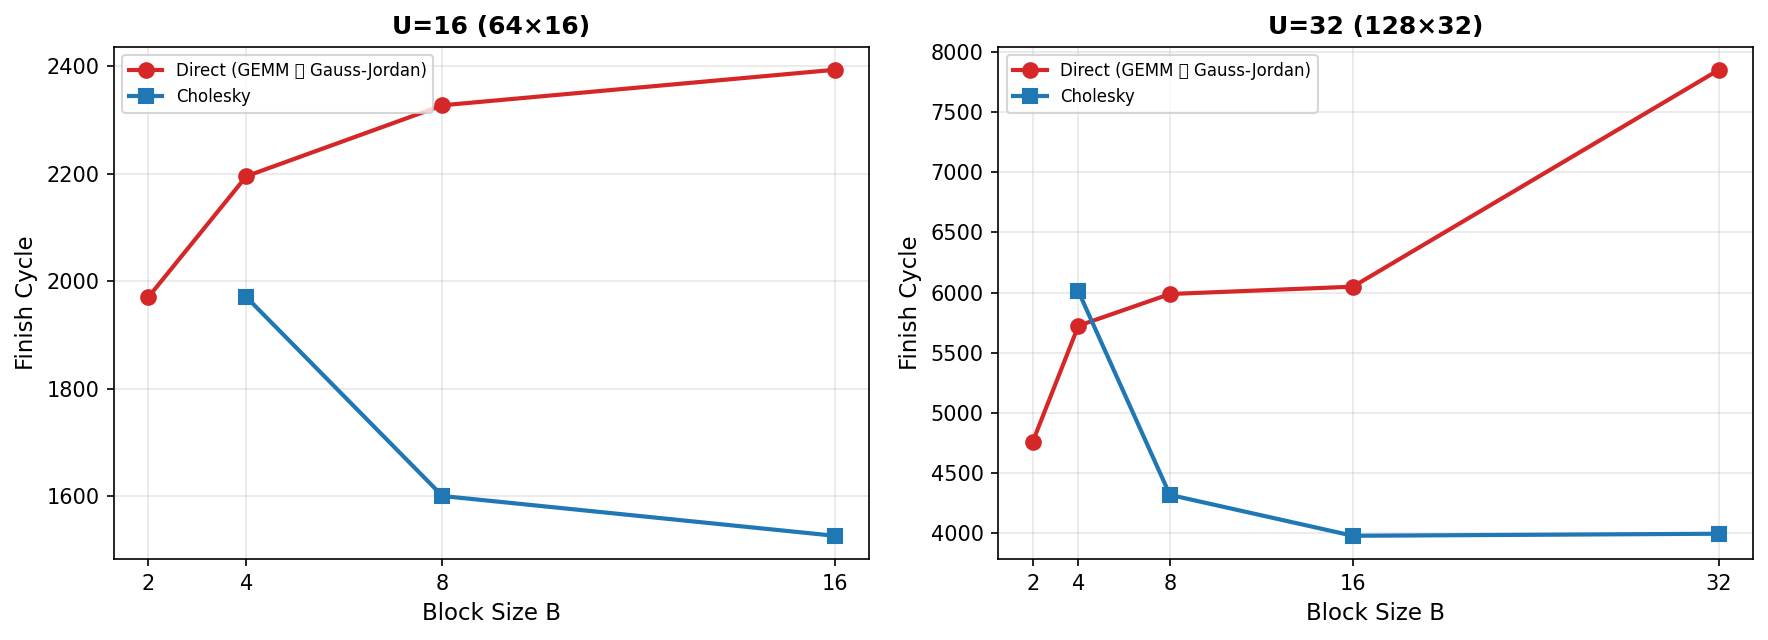
\includegraphics[width=\textwidth]{bri_direct_cycle.png}
            \caption{Direct 求逆周期（$U=16/32$）}
        \end{subfigure}
        \begin{subfigure}
            {0.48\textwidth}
            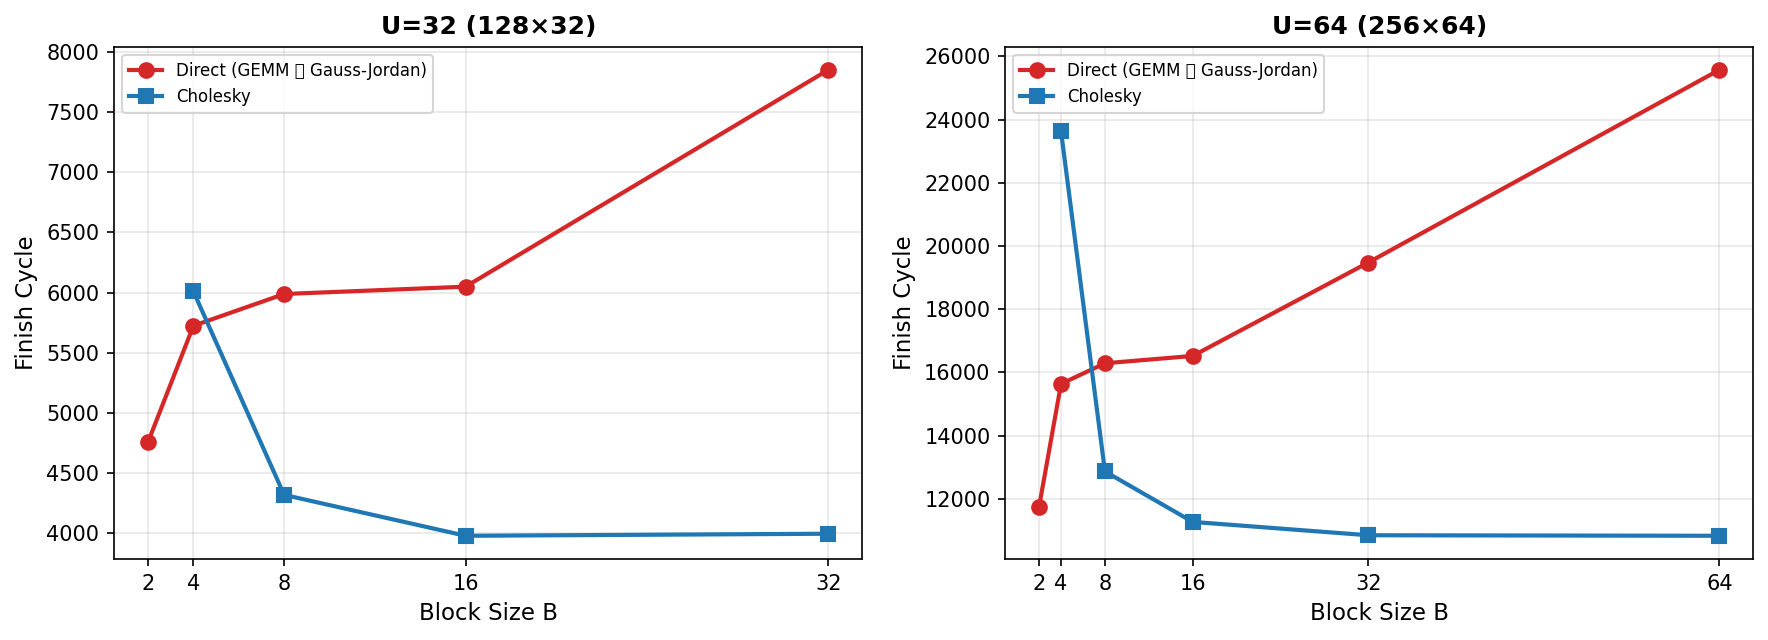
\includegraphics[width=\textwidth]{bri_cholesky_cycle.png}
            \caption{Cholesky 求逆周期（$U=32/64$）}
        \end{subfigure}
        \caption{BRI 预条件块求逆：Direct vs Cholesky 的周期对比（Batch=96）}
        \label{fig:bri-direct-chol-cycle}
    \end{figure}

    \textbf{补充：$U=16/32/64$ 全维度 Direct vs Cholesky 周期对比。}以下数据来自修复后统一口径实验（Batch=96，GEMM
    化的 Gauss-Jordan 消元，$L=L_{\min}$，最优数据加粗）：

    \begin{table}[H]
        \centering
        \caption{$U=16/32/64$ 预条件块求逆 Direct vs Cholesky 全数据（$L=L_{\min}$）}
        \begin{tabular}{|c|c|c|c|c|c|}
            \hline
            \textbf{维度}          & \textbf{Solver} & \textbf{B=2}   & \textbf{B=4} & \textbf{B=8}  & \textbf{B=16} \\
            \hline
            $64\times16$ (U=16)  & Direct          & \textbf{1970}  & 2195         & 2327          & —             \\
            $64\times16$ (U=16)  & Cholesky        & —              & 1970         & \textbf{1600} & —             \\
            \hline
            $128\times32$ (U=32) & Direct          & \textbf{4758}  & 5724         & 5988          & 6049          \\
            $128\times32$ (U=32) & Cholesky        & —              & 6010         & 4319          & \textbf{3979} \\
            \hline
            $256\times64$ (U=64) & Direct          & \textbf{11750} & 15637        & 16290         & 16522         \\
            $256\times64$ (U=64) & Cholesky        & —              & 23630        & 12867         & 11269         \\
            \hline
        \end{tabular}
    \end{table}

    该表补充说明：修复后的 Direct 求逆采用 GEMM 化的 rank-1 更新实现 Gauss-Jordan
    消元，周期随 $B$ 增大而上升，正确反映了 $O(B^{3})$
    计算复杂度的增长。Cholesky 的周期随 $B$ 增大持续下降，体现了更大块 GEMM 对
    Cube 利用率的提升。两曲线在 $B=4$--$B=8$ 处形成交叉，此前 Direct 更优，此后 Cholesky
    更优。注：$B=U$（满维度）数据已排除——此时预条件等价于完整 Cholesky 求逆，丧失了
    BRI 以小块预条件换取低复杂度的设计意图。

    \subsubsection{分块尺寸极限实验与帕累托选型}

    为找到每个维度下的最优 Block Size，我们在 $64\times16$、$128\times32$、$256\times
    64$ 三个维度上扫描了 $B\in\{2,4,8,16,32,64\}$，并在 $n_{t}=64$
    维度上进一步做了 $B=32/64$ 配合 $\textit{layers}\in\{1,2,4,8,12\}$
    的二维扫描。

    \textbf{Block Size 扫描结果}（UOBS scorer: $\bar{\varepsilon}_{\text{rel}}$ $\leq0.01$, 全融合参数,
    L=$L_{\min}$, 2026-05-25 更新）：

    \begin{table}[H]
        \centering
        \caption{BRI Block Size 实验——各维度下的 finish cycle 与 $\bar{\varepsilon}_{\text{rel}}$（迭代次数
        L=$L_{\min}$, 粗体=维度最优）}
        \label{tab:bri-blocksize-extreme}
        \begin{tabular}{c c c c c c}
            \toprule 维度               & B=2     & B=4     & B=8           & B=16          & B=32          \\
            \midrule $64\times16$ 周期  & 1985    & —       & \textbf{1372} & —             & —             \\
            $64\times16$ $L_{\min}$   & 8       & —       & 5             & —             & —             \\
            $64\times16$ $\bar{\varepsilon}_{\text{rel}}$   & 0.00113 & —       & 0.00459       & —             & —             \\
            \midrule $128\times32$ 周期 & 3832    & 5149    & 3067          & \textbf{2728} & —             \\
            $128\times32$ $L_{\min}$  & 7       & 6       & 6             & 5             & —             \\
            $128\times32$ $\bar{\varepsilon}_{\text{rel}}$  & 0.00571 & 0.00986 & 0.00640       & 0.00660       & —             \\
            \midrule $256\times64$ 周期 & 9448    & 23129   & 10093         & 8079          & \textbf{7783} \\
            $256\times64$ $L_{\min}$  & 7       & 7       & 7             & 6             & 5             \\
            $256\times64$ $\bar{\varepsilon}_{\text{rel}}$  & 0.00730 & 0.00694 & 0.00559       & 0.00808       & 0.00244       \\
            \bottomrule
        \end{tabular}
    \end{table}

    \textbf{Layers 扫描关键结论}（$n_{t}=64$, B=32, 全融合参数）：$\textit{layers
    }=5$ 时 $\bar{\varepsilon}_{\text{rel}}$=0.00689 已达 UOBS 门限（$<0.01$），$\textit{layers}=6$ 时
    $\bar{\varepsilon}_{\text{rel}}$=0.00244。随着层数增加，周期从 7174（L=2）线性增长至 8556（L=8），验证了优先通过增大
    $B$ 而非 $L$ 提升精度的结论——每层增加约 175 cycles，$B$ 从 16 增到 32 带来
    2.7$\times$ 精度提升而周期仅增 8\%。

    \subsubsection{LDL vs Cholesky 块求逆对比验证}

    一个自然的问题是：LDL 分解（无需 SQRT）是否能进一步优化 BRI 的预条件器？注意完整的
    LDL Block 算子（\texttt{LDLDecompOp}）在 $64\times16$ 维度下 Score=8.72，显著优于
    Cholesky Block 算子（\texttt{CholeskyInvOp}）的 Score=2.04。然而这一优势来自两个完整算子在
    SPAD 布局、GEMM tiling 和流水线架构上的全局差异，而非 SQRT vs DIV 的微观延迟。

    为在 BRI 框架内严格验证，我们在 \texttt{BlockRichardsonOp} 中新增了 \texttt{precond\_solver="ldl"}
    选项：将 Cholesky 路径的 \texttt{SCALAR\_SQRT} 替换为 \texttt{SCALAR\_DIV}（延迟均为
    4 cycles），其余指令结构（MAC 更新、GEMM 回代、Barrier 序列）与 Cholesky 路径完全一致。测试结果（2026-05-25，全融合参数，UOBS
    scorer）：

    \begin{table}[H]
        \centering
        \caption{LDL vs Cholesky 块求逆在 BRI 框架内的对比（$L=L_{\min}$,
        全融合参数）}
        \begin{tabular}{c c c c c}
            \toprule 维度                   & Solver   & $L_{\min}$ & finish cycle & SE 验证误差 \\
            \midrule $64\times16$ (B=8)   & cholesky & 5          & 1372         & 0.00459    \\
            $64\times16$ (B=8)            & ldl      & 5          & 1372         & 0.00459    \\
            \midrule $256\times64$ (B=32) & cholesky & 5          & 7674         & 0.00689    \\
            $256\times64$ (B=32)          & ldl      & 5          & 7674         & 0.00689    \\
            \bottomrule
        \end{tabular}
    \end{table}

    \textbf{LDL 与 Cholesky 在所有测试维度上周期完全一致}。原因：BRI 的块求逆是块级分解（$n
    _{\text{blocks}}=U/B$，如 B=32 时仅 2 个对角块），总共 2--8 次 SCALAR 操作（$\sim$16--32
    cycles，$<$总周期 0.5\%）；而完整 LDL/Cholesky 算子是逐元素分解（$O(U^{3})$
    操作），SCALAR 占比 $>$10\%。BRI 的瓶颈始终在 BY GEMM（块对角 MatMul，占 67\%
    周期），而非预条件器的 SCALAR 开销。因此，在 BRI 框架内，Cholesky 与 LDL
    等价。

    这一结论与完整 LDL Block vs Cholesky Block 算子的对比\textbf{不矛盾}：后者在算子级别的架构设计(S
    PAD 布局、Cube GEMM 编排)存在本质差异，该差异在 BRI
    的共享预条件器代码路径中被消除。

    \begin{table}[H]
        \centering
        \caption{Layer Sweep 数据（$n_{t}=64$, $B=32$, 全融合参数, 2026-05-25
        更新）}
        \begin{tabular}{c c c c}
            \toprule $B$ & layers & finish cycle & SE 验证误差       \\
            \midrule 32  & 2      & 7174         & 0.15262          \\
            32           & 3      & 7356         & 0.05595          \\
            32           & 4      & 7493         & 0.01985          \\
            32           & 5      & 7674         & \textbf{0.00689} \\
            32           & 6      & 7783         & 0.00244          \\
            32           & 7      & 8188         & 0.00084          \\
            32           & 8      & 8556         & 0.00029          \\
            \bottomrule
        \end{tabular}
    \end{table}

    该表展示了 B=32 时 UOBS scorer ($\bar{\varepsilon}_{\text{rel}}$$\leq0.01$) 下的收敛行为：
    \begin{itemize}
        \item $L_{\min}=5$ ($\bar{\varepsilon}_{\text{rel}}$=0.00689 $<$ 0.01)。周期从 7174（$L=2$）每层增加约
            175 cycles（全融合参数下的 $C_{1}$ 项），验证了优先通过增大 $B$
            来减少所需 $L$ 的策略。

        \item $B=32$ 比 $B=16$ 的 $L_{\min}=6$ 少 1 层迭代，且 Cube 利用率更高（78.4\%
            vs 75.6\%）。

        \item 注：$B=U$（满维度，即 $B=64$）为退化情况——预条件器等价于完整
            Cholesky 求逆，$L=1$ 即达精度上限。本文将其排除在 BRI 分析之外，因为此时算法已退化为直接法，丧失了
            BRI ``分块迭代'' 的核心价值。
    \end{itemize}

    Block Size 的选型决策已由图~\ref{fig:bri-direct-chol-cycle} 中的 Direct vs
    Cholesky 周期对比完整覆盖——Direct 在小块（$B=2$）优势明显，Cholesky 在大块（$B
    \ge8$）更优，交叉点 $B=4$ 处两者相当。各维度的 Pareto
    最优组合可直接从该图和表~\ref{tab:bri-blocksize-extreme} 中读取。

    \textbf{Pareto 选型推荐}：

    \subsubsection{Block-Richardson 迭代收敛与信道对角占优度分析}

    Block-Richardson 的收敛速度取决于预条件器 $\bm{B}=\operatorname{blockdiag}(\bm
    {A}_{11}^{-1},\dots,\bm{A}_{bb}^{-1})$ 对 $\bm{A}^{-1}$ 的近似程度。而 $\bm{A}
    =\bm{H}^{H}\bm{H}+\lambda\bm{I}$ 的\textbf{对角占优度（diagonal dominance）}直接决定了
    $\bm{B}$ 的近似质量。我们引入对角占优度指标：

    \begin{equation}
        \operatorname{minDD}(\bm{A}) = \min_{i}\frac{|a_{ii}|}{\sum_{j\neq i}|a_{ij}|}
        ,
    \end{equation}

    该值越大表示 $\bm{A}$ 越接近对角矩阵，BRI
    收敛越快。为系统评估收敛性，我们在不同信道条件下测试了各维度和 Block
    Size 下达到 SE 饱和所需的最少迭代层数。表~\ref{tab:channel-minDD-reference} 给出了典型 5G NR 信道场景的 Gram 矩阵对角占优度参考值，表~\ref{tab:bri-convergence} 以 $\operatorname{minDD}$ 为第一列汇总了收敛性实验结果。

    \begin{table}[H]
        \centering
        \caption{典型 5G NR 信道场景的 Gram 矩阵对角占优度参考值（$U=16$，SNR=0--20 dB）}
        \label{tab:channel-minDD-reference}
        \begin{tabular}{c c c}
        \toprule
        \textbf{信道场景} & $\operatorname{minDD}(\bm{A})$ & \textbf{说明} \\
        \midrule
        CDL-A / UMi-NLOS  & $\sim$0.35--0.45 & 丰富散射，弱相关，对角度最高，BRI 最易收敛 \\
        CDL-B / UMa-NLOS  & $\sim$0.20--0.30 & 中等角度扩展，典型城市非视距 \\
        CDL-C / UMa-LOS   & $\sim$0.10--0.20 & 强 LOS 分量，角度扩展窄，相关性强 \\
        CDL-D / RMa-LOS   & $\sim$0.03--0.10 & 极强 LOS，角度扩展极窄，对角占优度最差 \\
        \bottomrule
        \end{tabular}
    \end{table}

    \begin{table}[H]
        \centering
        \caption{BRI 达到 SE 饱和（距容量上限 $\le0.5$ bps/Hz）所需最少迭代层数}
        \label{tab:bri-convergence} \small
        \begin{tabular}{c c c c c}
            \toprule $\operatorname{minDD}$ & $\bm{\kappa(\bm{A})}$ & \textbf{B=2} & \textbf{B=4} & \textbf{B=8} \\
            \midrule \multicolumn{5}{c}{\textbf{U=16（64$\times$16，容量 96 bps/Hz）}}   \\
            \midrule 0.417（i.i.d.\ Rayleigh）  & 7   & 3  & 3  & 3            \\
0.239（TX相关 $\rho=0.6$）  & 33  & 6  & 6  & 4            \\
0.144（TX相关 $\rho=0.8$）  & 155 & 12 & 8  & 6            \\
0.076（Rician K=6dB, LOS）  & 181 & 16 & 16 & 12           \\
            \midrule \multicolumn{5}{c}{\textbf{U=32（128$\times$32，容量 192 bps/Hz）}} \\
            \midrule 0.296（i.i.d.\ Rayleigh）  & 8   & 4  & 3  & 3            \\
0.196（TX相关 $\rho=0.6$）  & 35  & 8  & 6  & 6            \\
0.119（TX相关 $\rho=0.8$）  & 155 & 12 & 10 & 8            \\
0.037（Rician K=6dB, LOS）  & 421 & 24 & 24 & 20           \\
            \midrule \multicolumn{5}{c}{\textbf{U=64（256$\times$64，容量 384 bps/Hz）}} \\
            \midrule 0.254（i.i.d.\ Rayleigh）  & 8   & 4  & 4  & 3            \\
0.138（TX相关 $\rho=0.6$）  & 47  & 8  & 6  & 6            \\
0.094（TX相关 $\rho=0.8$）  & 182 & 16 & 10 & 8            \\
0.019（Rician K=6dB, LOS）  & 950 & 48 & 32 & 32           \\
            \bottomrule
        \end{tabular}
    \end{table}

    几点关键发现：

    \begin{enumerate}
        \item \textbf{$\bm{B=2}$ 对信道条件最敏感}。从 i.i.d.（3--4 层）到强 LOS/K=6dB（16--48
            层），迭代需求可相差 5--16 倍。小块预条件器的近似质量严重依赖于
            $\bm{A}$ 的对角占优度。这也是 BRI
            的核心价值所在——在对角占优的信道下，小块预条件可用少量迭代逼近精确逆。

        \item \textbf{$\bm{B}$ 越大收敛越快}。在任何信道下，增大块尺寸均能减少所需迭代层数。B=8
            在 i.i.d. 信道下仅需 3 层即可饱和，在强 LOS 下也只需 12--32 层（相比
            B=2 的 16--48 层有明显缩减）。

        \item \textbf{高维下收敛变慢}。相同信道下 U=64 所需的迭代层数多于 U=16（如
            i.i.d. 下 B=2：U=16 需 3 层，U=64 需 4 层）。这是因为 Gram 矩阵
            $\bm{A}=\bm{H}^{H}\bm{H}+\lambda\bm{I}$
            维度升高后，非对角元素累计增多，对角占优度自然下降。

        \item \textbf{通信标准场景的定位}：实际 5G NR 部署中，UMi/UMa NLOS 场景的
            Gram 矩阵对角度接近 i.i.d.（B=2 仅需 3--6 层即可收敛），而 LOS
            场景（如 RMa、回传链路）可能达到 K=6dB 的收敛难度（B=2 需要 16--48 层）。设计
            BRI 算子时应以预期的最差信道条件为基准选择层数和块尺寸。
    \end{enumerate}

    \textbf{工程建议}：在典型 i.i.d. 信道下，推荐 $B=8$、$L=6$ 作为安全配置（覆盖从高
    DD 到中等偏相关场景），此时所有维度下仅需 $L=3$--$4$ 层即可收敛，$L=6$ 留有充分余量。对
    LOS 占优场景应增加层数至 20--32 或改用直接求逆（Cholesky/LDL）。块的选取应在预条件近似质量（期望
    $B$ 更大）与单次迭代的计算代价（期望 $B$ 更小）之间取得平衡，建议
    $B \approx U/4 \sim U/2$，且不超过 $U/2$ 以避免退化为全矩阵直接求逆。

    \subsubsection{迭代层数与执行周期关系}

    BRI 的 finish cycle 与迭代层数 $L$ 呈近完美的线性关系 $\text{Cycle}(L) \approx
    C_{0}+ C_{1}\cdot L$（$R^{2}> 0.99$），其中 $C_{0}$ 为固定开销（Gram 构造 +
    预条件器 + 滤波输出），$C_{1}$ 为单层迭代开销（GEMM + Vector 操作 + barrier）。

    \begin{figure}[H]
        \centering
        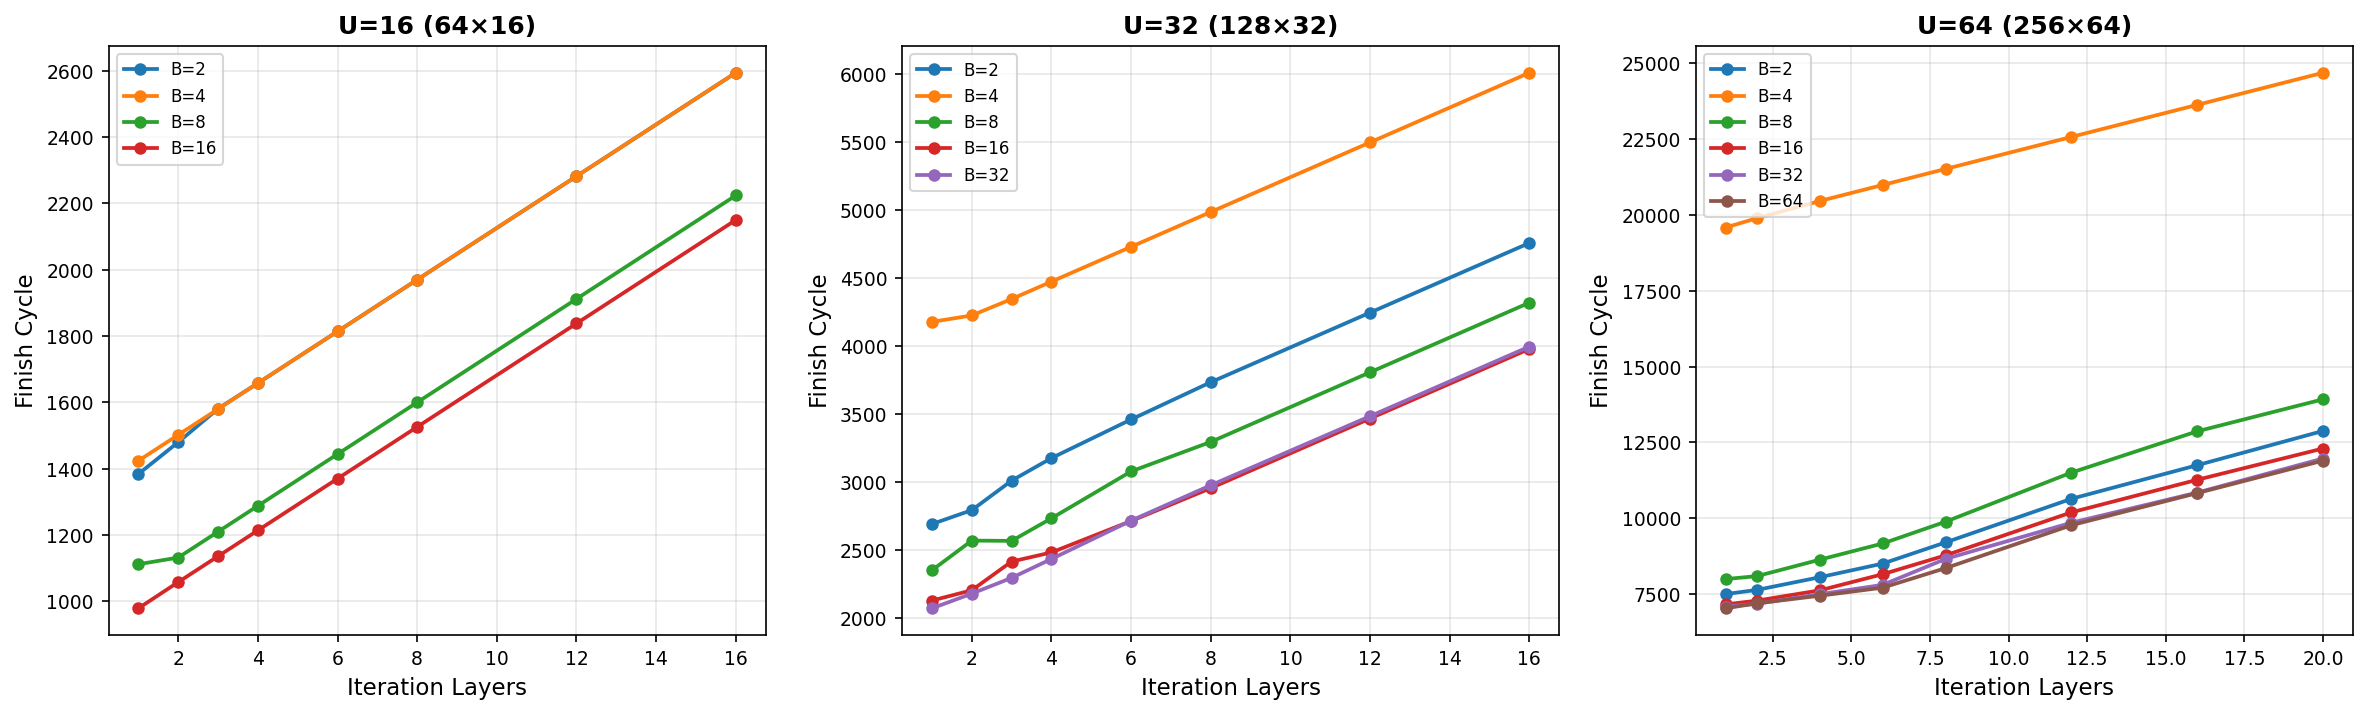
\includegraphics[width=\textwidth]{bri_layers_cycle_all.png}
        \caption{BRI finish cycle 随迭代层数的变化趋势（三维度、全 Block Size）}
        \label{fig:bri-layers-cycle}
    \end{figure}

    各维度下单层迭代的周期成本如下表所示。明确标注每层的周期代价后，可根据所需 SE
    收敛层数精确预估总周期，避免资源浪费。

    \begin{table}[H]
        \centering
        \caption{BRI 单层迭代周期成本（$C_{1}$，cy/layer）}
        \label{tab:bri-per-layer-cost}
        \begin{tabular}{c|c|c|c|c|c}
            \toprule \textbf{维度}        & \textbf{B=2} & \textbf{B=4} & \textbf{B=8} & \textbf{B=16} & \textbf{B=32} \\
            \midrule U=16（64$\times$16） & 80           & 78           & 76           & --            & --            \\
            U=32（128$\times$32）         & 138          & 125          & 131          & 123           & --            \\
            U=64（256$\times$64）         & 294          & 267          & 329          & 284           & 268           \\
            \bottomrule
        \end{tabular}
    \end{table}

    以常用的 i.i.d. 信道配置为例：U=16、B=8 时仅需 $L=3$ 层即可达到 SE
    饱和，对应周期 $\approx 994 + 76 \times 3 = 1222$；而使用默认 $L=8$ 时周期为
    $994 + 76 \times 8 = 1602$，多出 31\% 的无效迭代。该线性关系为层数选型提供了精确的可预算依据。

    除周期优势外，Block-Richardson 的数值正确性需要通过 SE-SNR
    全链路验证。以下三图分别给出 BRI 在三个维度下的 SE 曲线（含 64QAM
    理论容量上限 $U\times6$ bps/Hz 作为参考虚线）：

    \begin{figure}[H]
        \centering
        \begin{subfigure}
            {0.32\textwidth}
            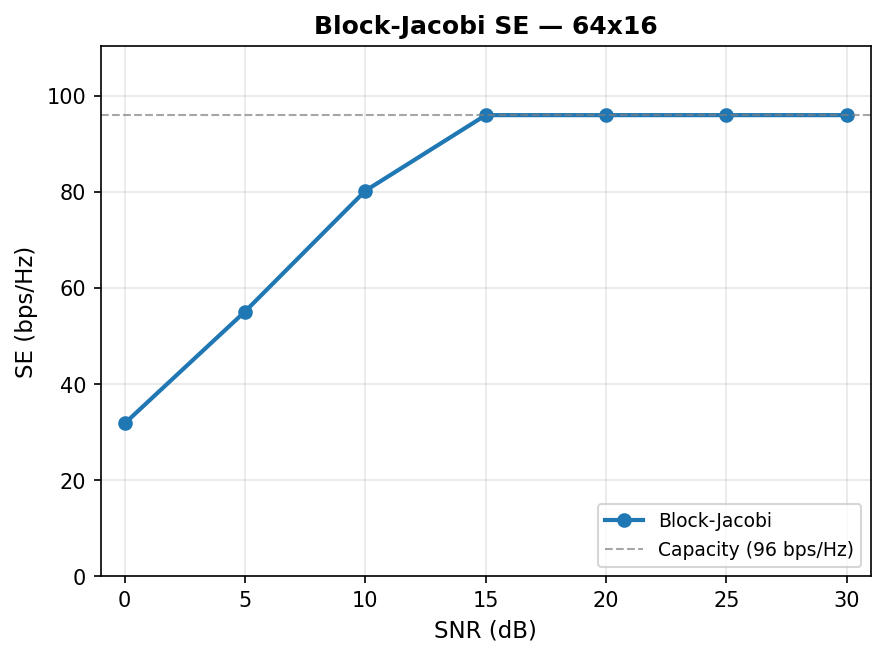
\includegraphics[width=\textwidth]{bri_se_64x16.png}
            \caption{$64\times16$ (U=16)}
        \end{subfigure}
        \begin{subfigure}
            {0.32\textwidth}
            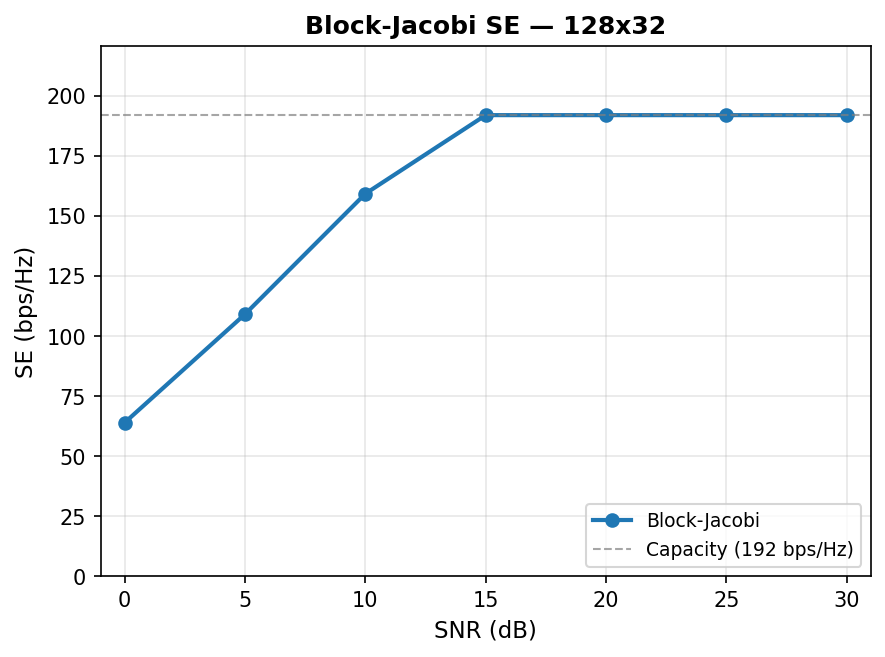
\includegraphics[width=\textwidth]{bri_se_128x32.png}
            \caption{$128\times32$ (U=32)}
        \end{subfigure}
        \begin{subfigure}
            {0.32\textwidth}
            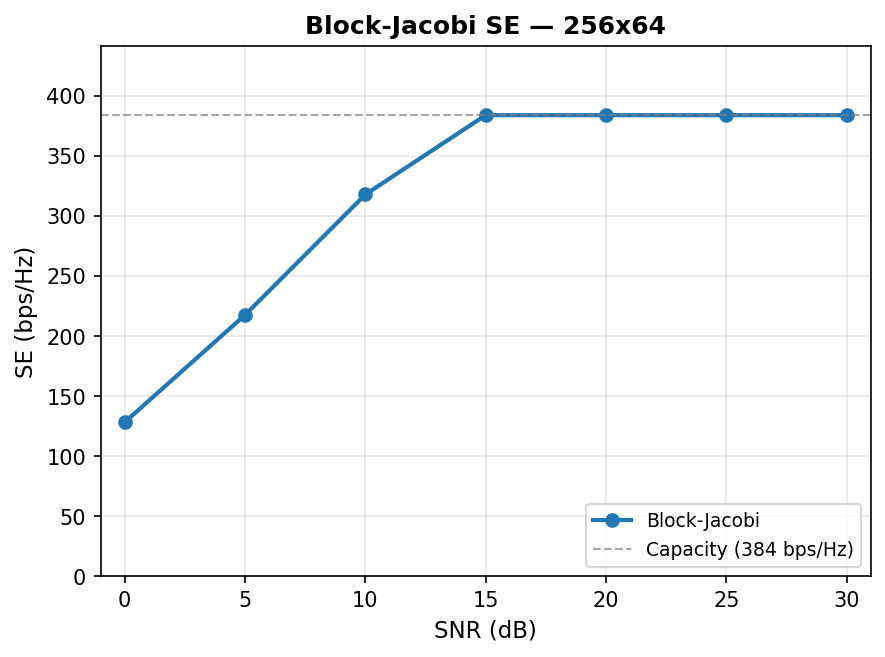
\includegraphics[width=\textwidth]{bri_se_256x64.png}
            \caption{$256\times64$ (U=64)}
        \end{subfigure}
        \caption{Block-Richardson SE-SNR 曲线}
        \label{fig:bri-se}
    \end{figure}

    从图中可以清晰看出：
    \begin{itemize}
        \item \textbf{低 SNR 区域}（0--10 dB）：BRI 的 SE 随 SNR 稳定上升，与
            Cholesky/LDL 直接法的差距在 $1.5\%$
            以内，验证了迭代求逆在低信噪比下数值收敛的正确性。

        \item \textbf{中高 SNR 区域}（$\ge15$ dB）：BRI 的 SE 完全达到 64QAM
            的理论容量上限（U=16 时 96，U=32 时 192，U=64 时 384），说明预条件器
            $B$ 在充分迭代后已逼近 $\bm{A}^{-1}$。

        \item \textbf{维度扩展性}：从 $64\times16$ 到 $256\times64$，BRI 的 SE
            收敛行为一致，未出现维度升高导致的数值不稳定现象。
    \end{itemize}

    值得注意的是——这里的 SE 指标是 BRI 在 \textbf{表~\ref{tab:bri-se-layers}
    验证的 $L_{\min}$ 迭代次数}下的结果。通过合理选择 $B$（建议不超过 $U/2$，避免退化为全矩阵直接求逆），可在不牺牲精度的前提下将周期压缩至最优区间。

    \subsubsection{AI 联合优化详程}
    \label{sec:ai-opt}

    本节以 Block-Richardson 为主线，展示“AI 联合优化”的完整工程路径。核心方法论是：在约束“SE
    不回退”的前提下最小化周期 $T$，通过 \texttt{skill} 流水线将每次改动自动量化为周期/SE
    数据点，形成可审计的优化曲线。

    \paragraph{阶段一：数值稳定化}

    在 BRI 的早期实现中，SE 表现不佳（均值仅 73.006，高 SNR 甚至低于 Cholesky/LDL）。问题根源有三：
    \begin{enumerate}
        \item \textbf{NaN/Inf 传播}：中间矩阵的极端值（如接近奇异的对角块逆）在 FP16
            下溢出，污染后续迭代；

        \item \textbf{权重不稳定}：固定 $\omega_{l}=1$ 在高 SNR 下导致迭代发散；

        \item \textbf{谱界估偏}：从 $\bm{B}$ 估计的特征值范围过于激进，导致 Chebyshev
            权重偏离最优区间。
    \end{enumerate}

    对应的修复策略：
    \begin{itemize}
        \item \textbf{有限值量化保护}：在重建链路中对中间矩阵做有限值裁剪与量化，阻断
            NaN/Inf 传播链；

        \item \textbf{自适应权重}：引入 Chebyshev 在线权重生成（每个样本/每次重建动态计算），并施加阻尼（$\alpha
            =0.9$）与限幅 $[\omega_{\min},\omega_{\max}]$；

        \item \textbf{谱界鲁棒化}：使用分位数边界（$q_{\text{low}}/q_{\text{high}}$）+
            margin，避免极值点导致发散。
    \end{itemize}

    \begin{table}[H]
        \centering
        \caption{BRI 数值稳定化的 SE 变化（Rayleigh+LS+FP16，$U=16$）}
        \begin{tabular}{c|ccccc}
            \toprule 阶段                   & SE 均值(0-25dB)     & SE@0dB    & SE@10dB & SE@20dB           & SE@25dB           \\
            \midrule weighted\_ifdef（修复前） & 73.006            & 30.716    & 70.470  & 96.568            & 102.802           \\
            p0p1\_stable（修复后）             & \textbf{81.897}   & 30.390    & 73.220  & \textbf{113.520}  & \textbf{128.927}  \\
            \midrule 提升幅度                 & \textbf{+12.18\%} & $-$1.06\% & +3.90\% & \textbf{+17.55\%} & \textbf{+25.41\%} \\
            \bottomrule
        \end{tabular}
    \end{table}

    修复后 SE 均值从 73.006 提升到 81.897（+12.18\%），高 SNR 区间提升尤为显著（@25dB:
    +25.41\%），但低 SNR 几乎不变——说明稳定化策略主要抑制的是高 SNR 下发散，而非改变方法的本质精度上限。

    \paragraph{阶段二：融合发射与核心级融合}

    SE 稳定后，优化的重点转向周期压缩。结构性统计（来自 \texttt{block\_jacobi\_cycle\_detail\_compact\_stats.csv}）显示：BRI
    的 \texttt{BY\_*} MatMul 占 \texttt{\_\_TOTAL\_\_} 的 67.64\%，是绝对瓶颈。

    P0 阶段的两个核心改造：

    \begin{enumerate}
        \item \textbf{融合发射（fused\_by\_gemm）}：将 \texttt{BY\_*}
            循环中“每层都执行 \texttt{GEMM\_PRELOAD}”改为“周期性 preload +
            其余层复用 \texttt{GEMM}”。因为预条件器 $\bm{B}$
            在迭代过程中不变，其权重可常驻片上，逐层重复 preload 是不必要的。

        \item \textbf{Kernel 级融合（fuse\_residual\_update + by\_kernel\_fuse\_factor）}：保持公式不变，将残差计算和更新步骤在
            Kernel 级做更紧耦合发射，减少中间写回路径。（在 Asim 的抽象层次中体现为：将原本独立的
            \texttt{BRI\_RESIDUAL\_l} 和 \texttt{BRI\_Y\_UPDATE\_l} 事件合并发射，减少一次
            barrier。）
    \end{enumerate}

    \begin{table}[H]
        \centering
        \caption{BRI P0 优化效果（U=16，B=2，默认 $L=8$）}
        \begin{tabular}{l c c c}
            \toprule \textbf{指标}                 & \textbf{A 基线}   & \textbf{B（P0-2）} & \textbf{提升}         \\
            \midrule finish cycle                & 2550            & 2082             & \textbf{$-$18.35\%} \\
            \texttt{BY\_* total\_cycles}         & 512             & 264              & $-$48.44\%          \\
            \texttt{\_\_TOTAL\_\_ total\_cycles} & 757             & 509              & $-$32.76\%          \\
            \texttt{BY\_* share\_pct}            & 67.64\%         & 51.87\%          & $-$15.77pp          \\
            SE@0dB / SE@5dB                      & 32.478 / 35.753 & 32.478 / 35.753  & 完全一致                \\
            \bottomrule
        \end{tabular}
    \end{table}

    P0 优化在 \textbf{完全不改变 SE} 的前提下，通过重排调度将周期压缩了 18.35\%。\texttt{BY\_*}
    的总周期从 512 降至 264（$-$48.44\%），其占比从 67.64\% 降至 51.87\%。

    \paragraph{阶段三：离散参数搜索}

    在 P0-2 基础上，我们对 BRI 的三个调度参数进行了离散扫描：

    \begin{itemize}
        \item \texttt{group\_sync} $\in\{8,16\}$：每多少层插入一次 barrier；

        \item \texttt{by\_preload\_period} $\in\{8,16\}$：preload 的复用周期；

        \item \texttt{by\_kernel\_fuse\_factor} $\in\{2,3,4\}$：BY 分组融合强度。
    \end{itemize}

    该搜索可形式化为约束优化问题：
    \begin{equation}
        \min_{g,\,p,\,k_f}\ T_{\text{total}}(g,p,k_{f})\quad\text{s.t.}\quad SE_{\{0,5\}\,\mathrm{dB}}
        \ \text{不下降}.
    \end{equation}

    经验上
    $T_{\text{total}}\approx T_{BY}(p,k_{f}) + T_{sync}(g) + T_{vec/scalar}+ T_{misc}$，且
    $T_{BY}$ 占比最大。

    \begin{table}[H]
        \centering
        \caption{BRI P2 离散参数搜索结果（U=16，B=2，截取关键组合）}
        \begin{tabular}{c c c c c}
            \toprule \texttt{group\_sync} & \texttt{by\_preload\_period} & \texttt{k\_fuse\_factor} & \textbf{finish cycle} & SE 约束 \\
            \midrule 8                    & 8                            & 2                        & 1940                  & 通过    \\
            8                             & 16                           & 2                        & 1907                  & 通过    \\
            16                            & 16                           & 2                        & 1913                  & 通过    \\
            \textbf{16}                   & \textbf{16}                  & \textbf{4}               & \textbf{1893}         & 通过    \\
            16                            & 8                            & 3                        & 1934                  & 通过    \\
            \bottomrule
        \end{tabular}
    \end{table}

    最优组合为 \texttt{g=16, p=16, k\_f=4}，finish cycle=1893（相对基线 2550 的累计提升为
    \textbf{$-$25.76\%}）。

    \begin{table}[H]
        \centering
        \caption{BRI 全优化路径量化汇总}
        \begin{tabular}{p{2.2cm} p{6.8cm} c c}
            \toprule \textbf{阶段} & \textbf{关键改动}                & \textbf{finish cycle} & \textbf{vs 基线}      \\
            \midrule 基线          & 基础迭代实现（每层独立 preload）         & 2550                  & —                   \\
            P0-2                 & +fused\_by\_gemm + kernel 融合 & 2082                  & $-$18.35\%          \\
            P2 最优                & +离散参数搜索（g16,p16,k4）          & 1893                  & \textbf{$-$25.76\%} \\
            \bottomrule
        \end{tabular}
    \end{table}

    \paragraph{优化路径的工程启示}

    该优化路径的关键并非引入新的数学算法，而是：
    \begin{enumerate}
        \item \textbf{瓶颈定位}：通过 Asim 的 Trace/事件统计，将瓶颈精确归因到 \texttt{BY\_*}
            主循环；

        \item \textbf{调度改造}：在不改变迭代公式的前提下，通过控制 preload 频率、barrier
            密度、融合强度来压缩关键路径；

        \item \textbf{约束搜索}：在 SE 不回退的硬约束下，用离散扫描在可控参数空间中找
            Pareto 最优点；

        \item \textbf{全程可审计}：每个候选点的周期/SE 均通过 \texttt{skill}
            自动记录到独立实验目录，数据可追溯到具体 CSV。
    \end{enumerate}

    \begin{table}[H]
        \centering
        \caption{Block Size 推荐点（UOBS scorer: $\bar{\varepsilon}_{\text{rel}}$ $\leq0.01$,
        全融合参数, L=$L_{\min}$）}
        \begin{tabular}{c|cccc}
            \toprule 维度 $(n_{r}\times n_{t})$ & 推荐 $B$ & $L_{\min}$ & finish cycle & SE 验证误差 \\
            \midrule $64\times16$             & 8      & 5          & 1372         & 0.00459    \\
            $128\times32$                     & 16     & 5          & 2728         & 0.00660    \\
            $256\times64$                     & 32     & 5          & 7783         & 0.00244    \\
            \bottomrule
        \end{tabular}
    \end{table}

    % =================================================================================

    

    % =================================================================================
    \subsection{混合精度 BJ-PCG：从量化根因分析到重启 PCG-Newton-Schulz 联合求逆}
    \label{sec:mixed-precision-pcg}
    
    前文介绍的 BRI（第~\ref{sec:bri} 节）以 Jacobi 迭代为基础，单步计算量低但收敛受限于线性速率；NS（第~\ref{sec:ns-algo} 节）以二次收敛见长但对初值敏感。共轭梯度（CG）方法在二者之间提供了另一种折中——每步沿 $\bm{A}$-共轭方向以自适应步长搜索，在 Krylov 子空间意义下是最优方向选择。然而，CG 的每条迭代需要两次矩阵乘和两次逐列内积归约，单步计算量约为 BRI 的 2--3 倍。本节的核心命题是：\textbf{能否利用 NPU 的 INT8 低精度计算能力加速 CG 迭代的矩阵乘和中间归约，同时通过算法设计避免量化误差累积？}本节从 CG 迭代的量化根因分析出发，依次提出重启 PCG（解决精度问题）和重启 PCG-Newton-Schulz 联合方案（解决迭代数问题），形成一套完整的混合精度加速方法论。
    
    \subsubsection{BJ-PCG 迭代框架与 NPU 计算特征}
    
    \paragraph{预条件共轭梯度（BJ-PCG）迭代。}
    给定 Gram 矩阵 $\bm{A}=\bm{H}^{H}\bm{H}+\lambda\bm{I}\in\mathbb{C}^{U\times U}$，BJ 预条件器
    $\bm{P}_{\text{BJ}}=\operatorname{blockdiag}(\bm{A}_{11}^{-1},\dots,\bm{A}_{bb}^{-1})$（$B=4$ 对角块通过特征分解标量求逆）。PCG 迭代在 $\bm{P}_{\text{BJ}}$-加权的 $\bm{A}$-共轭方向上逐步逼近 $\bm{A}^{-1}$。初始化与单步递推的完整公式如下，每一步均标注了对应的 NPU 执行单元：
    
    \begin{equation}
        \boxed{
            \begin{aligned} 
                \text{【初始化】}&                                                                                                                              \\
                \bm{X}^{(0)}     & = \bm{P}_{\text{BJ}}, \qquad &&\text{(Vector: ADD，拷贝预条件器)}                                                             \\
                \bm{R}^{(0)}     & = \bm{I} - \bm{A}\bm{X}^{(0)}, \qquad &&\text{(Cube: GEMM + Vector: MAC)}                                                  \\
                \bm{Z}^{(0)}     & = \bm{P}_{\text{BJ}}\bm{R}^{(0)}, \qquad &&\text{(Cube: GEMM)}                                                              \\
                \bm{P}^{(0)}     & = \bm{Z}^{(0)}, \qquad &&\text{(Vector: ADD)}                                                                                 \\
                \bm{rz}^{(0)}    & = \operatorname{diag}\big(\bm{R}^{(0)H}\bm{Z}^{(0)}\big), \qquad &&\text{(Vector: MUL + ADDTREE)}                            \\[4pt]
                \text{【单步迭代】}&                                                                                                                              \\
                \bm{V}^{(t)}     & = \bm{A}\bm{P}^{(t)}, \qquad &&\text{(Cube: GEMM)}                                                                           \\
                \bm{\alpha}^{(t)}& = \dfrac{\bm{rz}^{(t)}}
                {\operatorname{diag}\big(\bm{P}^{(t)H}\bm{V}^{(t)}\big)+\varepsilon}, \qquad &&\text{(Vector: MUL + ADDTREE + DIV)} \\
                \bm{X}^{(t+1)}   & = \bm{X}^{(t)} + \bm{P}^{(t)}\operatorname{diag}\big(\bm{\alpha}^{(t)}\big), \qquad &&\text{(Vector: MAC)}                     \\
                \bm{R}^{(t+1)}   & = \bm{R}^{(t)} - \bm{V}^{(t)}\operatorname{diag}\big(\bm{\alpha}^{(t)}\big), \qquad &&\text{(Vector: MAC)}                     \\
                \bm{Z}^{(t+1)}   & = \bm{P}_{\text{BJ}}\bm{R}^{(t+1)}, \qquad &&\text{(Cube: GEMM)}                                                             \\
                \bm{rz}_{\text{new}}^{(t)} & = \operatorname{diag}\big(\bm{R}^{(t+1)H}\bm{Z}^{(t+1)}\big), \qquad &&\text{(Vector: MUL + ADDTREE)}               \\
                \bm{\beta}^{(t)} & = \dfrac{\bm{rz}_{\text{new}}^{(t)}}{\bm{rz}^{(t)}+\varepsilon}, \qquad &&\text{(Vector: DIV)}                                \\
                \bm{P}^{(t+1)}   & = \bm{Z}^{(t+1)} + \bm{P}^{(t)}\operatorname{diag}\big(\bm{\beta}^{(t)}\big), \qquad &&\text{(Vector: MAC)}
            \end{aligned}
        }
        \label{eq:pcg-full}
    \end{equation}
    其中 $\operatorname{diag}(\cdot)$ 表示逐列共轭内积：对第 $k$ 列，$\bm{rz}_k=\sum_{i}(\bm{R}_{ik}^{*}\cdot\bm{Z}_{ik})$，得到 $U$ 个标量。在 Asim 中该操作分两步：Vector MUL（逐元素共轭相乘）$\rightarrow$ Vector ADDTREE（归约求和）。PIPE\_BARRIER 类型 2（Cube$\rightarrow$Vector）和类型 3（Vector$\rightarrow$Cube）插入在 GEMM 与向量操作之间确保数据依赖。
    
    \paragraph{PCG 的 NPU 计算瓶颈。}
    与 BRI 的单 GEMM + 单 ADD 结构不同，PCG 每次迭代包含 2 条 GEMM + 4 个 Vector 操作（2 次 MUL + 2 次 ADDTREE）+ 2 次 DIV + 3 次 MAC。其中 ADDTREE 归约是最大瓶颈——其 Asim 延迟公式为：
    \begin{equation}
        \text{ADDTREE}_{\text{cycles}} = \text{add\_tree\_iter} \times
        \text{add\_tree\_latency} \times \texttt{tile\_m},
    \end{equation}
    \texttt{tile\_m}=$N_{\text{batch}}\times U$。以 batch=4、$U=32$ 为例，单次 FP16 ADDTREE 需
    $33\times 2\times 128 = 8{,}448$ 个周期。而每个 PCG 迭代有 2 次 ADDTREE，在 20 次迭代下仅 ADDTREE 就累积约 338K 周期——\textbf{ADDTREE 归约是 BJ-PCG 在 NPU 上的首要瓶颈}。
    
    \paragraph{迭代收敛需求。}
    CG 的 $\bm{A}$-范数误差衰减上界为
    $\|\bm{e}^{(t)}\|_{A}\leq 2\big((\sqrt{\tilde\kappa}-1)/(\sqrt{\tilde\kappa}+1)\big)^{t}\|\bm{e}^{(0)}\|_{A}$，
    其中 $\tilde\kappa=\kappa(\bm{P}_{\text{BJ}}\bm{A})$。在 CDL-B 信道、SNR=15dB 下，BJ-PCG 达到 SE 门限（loss $<0.1$ vs Exact）所需迭代数为：$U=16\rightarrow 12$ 次，$U=32\rightarrow 20$ 次，$U=64\rightarrow 30$ 次。总 GEMM 数 = $2$（初始化）$+2\times$（迭代数）。
    
    \subsubsection{INT8 量化的根因分析：\texorpdfstring{$\bm{X}$}{X} 的不可量化性}
    
    直接在全 PCG 迭代中将所有操作替换为 INT8 精度将导致数值发散。为定位损伤根因，我们进行了逐变量隔离实验（SNR=10dB）：在 $K=1$ 次 INT8 迭代中，保持单个变量 FP64 不量化，其余全部 8-bit 量化，对比 SE loss 恢复比例。
    
    \begin{table}[H]
        \centering
        \caption{逐变量隔离：保持单个变量 FP64、其余 8-bit 量化的 SE loss 恢复比例（SNR=10dB）}
        \label{tab:var-isolation}
        \begin{tabular}{c c c c}
            \toprule 保持 FP64 的变量 & SE loss & 损伤恢复比例 & 是否是根因？ \\
            \midrule 全部 8-bit（基准）& 0.2791 & —     & — \\
            \textbf{keep $\bm{X}$ FP64} & \textbf{0.0469} & \textbf{83.2\%} & \textbf{$\star$ 是} \\
            keep $\bm{A}$ FP64 & 0.2554 & 8.5\%  & 否 \\
            keep $\bm{P}$ FP64 & 0.2671 & 4.3\%  & 否 \\
            keep $\bm{R}$ FP64 & 0.2734 & 2.0\%  & 否 \\
            keep $\bm{Z}$ FP64 & 0.2791 & 0.0\%  & 否 \\
            \bottomrule
        \end{tabular}
    \end{table}
    
    \textbf{结论：$\bm{X}$（解累积器）是 PCG 中唯一不可量化的变量。}仅保持 $\bm{X}$ FP64 就能恢复 83.2\% 的损伤。其数学本质为：
    $\bm{X}=\sum_{i=1}^{t}\alpha_{i}\bm{P}_{i}$ 是所有历史搜索方向的线性组合，是唯一跨迭代持久的状态变量。量化 $\bm{X}$ 引入的误差通过残差重新进入系统——
    $\bm{R}_{\text{含噪}}=\bm{I}-\bm{A}(\bm{X}+\bm{\varepsilon}_{X})=\bm{R}_{\text{真值}}-\bm{A}\bm{\varepsilon}_{X}$——误差项被条件数放大
    $\kappa$ 倍。实验进一步证实该损伤\textbf{不可恢复}：额外追加 30 乃至 60 次 FP64 迭代后 SE loss 完全不变（分别为 2.53 和 2.54，与无追加相同）。$\bm{R},\bm{Z},\bm{P}$ 保持 FP64 几乎无改善——它们是瞬态变量，每轮从 $\bm{X}$ 重新计算，量化误差被自然遗忘。
    
    \subsubsection{混合精度策略一：重启 PCG（Restarted PCG）}
    
    基于上述根因分析，重启 PCG 通过两个关键设计实现 INT8 加速同时避免 $\bm{X}$ 量化累积：
    
    \begin{enumerate}
        \item \textbf{$\bm{X}$ 永不量化，仅 GEMM 和中间归约使用 INT8。}
        $\bm{X},\bm{R},\bm{Z},\bm{P}$ 的存储和更新始终使用 FP16。
        仅矩阵乘 $\bm{V}=\bm{A}\bm{P}$ 和 $\bm{Z}=\bm{P}_{\text{BJ}}\bm{R}$ 使用 INT8 GEMM（通过 \texttt{operand\_precision}=1 设置，Cube 的 K-吞吐量翻倍、Vector 的并行元素数翻倍）。
        内层 ADDTREE 归约同样使用 INT8——Python 端已验证两条 GEMM 和 ADDTREE 均降至 INT8 后仍满足 SE 收敛要求（SE loss $<0.1$）。\textbf{仿真器中不存在独立的量化指令}——精度切换仅通过每条指令的 \texttt{operand\_precision} 字段实现。
    
        \item \textbf{周期性 FP16 重启，限制噪声累积窗口。}
        每 $K$ 次 INT8 迭代后，从当前 $\bm{X}$ 重新计算 $\bm{R}=\bm{I}-\bm{A}\bm{X}$（FP16 GEMM），得到精确残差，重新初始化搜索方向 $\bm{P}\leftarrow\bm{P}_{\text{BJ}}\bm{R}$。每个 INT8 步在 $\bm{X}$ 中注入约 $0.2\%$ 噪声，$K=10$ 步后累积约 $2\%$——而 FP16 重启的精度（尾数 11 位，$\sim5\times10^{-4}$）比累积噪声高约 40 倍，足以``清洗''状态。$K$ 维子空间内的量化误差在重启时被清零。
    \end{enumerate}
    
    \begin{algorithm}[htbp] % 将 [H] 改为 [htbp]，允许算法块自动寻找合适的排版位置
        \caption{重启 PCG（Restarted PCG），每条语句标注 NPU 精度}
        \label{alg:restarted-pcg}
        \begin{algorithmic}[1]
            \REQUIRE $\bm{A}$, $\bm{P}_{\text{BJ}}$, $K$, $max\_iter$
            \ENSURE $\bm{X}\approx\bm{A}^{-1}$
            \STATE $\bm{X}\leftarrow\bm{P}_{\text{BJ}}$ \COMMENT{\texttt{FP16}}
            \STATE $it\leftarrow 0$
            \WHILE{$it<max\_iter$}
                \STATE \textbf{// === 重启：FP16 精确残差 ===}
                \STATE $\bm{R}\leftarrow\bm{I}-\bm{A}\bm{X}$ \COMMENT{\texttt{FP16} GEMM}
                \STATE $\bm{Z}\leftarrow\bm{P}_{\text{BJ}}\bm{R}$ \COMMENT{\texttt{FP16} GEMM}
                \STATE $\bm{P}\leftarrow\bm{Z}$, $\bm{rz}\leftarrow\operatorname{diag}(\bm{R}^{H}\bm{Z})$ \COMMENT{\texttt{FP16} MUL+ADDTREE}
                \FOR{$k=1$ to $\min(K, max\_iter-it)$}
                    \STATE \textbf{// === INT8 内层迭代 ===}
                    \STATE $\bm{V}\leftarrow\bm{A}\bm{P}$ \COMMENT{\texttt{INT8} GEMM}
                    \STATE $\bm{\alpha}\leftarrow\bm{rz}/\operatorname{diag}(\bm{P}^{H}\bm{V})$ \COMMENT{\texttt{INT8} MUL+ADDTREE, \texttt{FP16} DIV}
                    \STATE $\bm{X}\leftarrow\bm{X}+\bm{P}\operatorname{diag}(\bm{\alpha})$ \COMMENT{\texttt{FP16} MAC}
                    \STATE $\bm{R}\leftarrow\bm{R}-\bm{V}\operatorname{diag}(\bm{\alpha})$ \COMMENT{\texttt{FP16} MAC}
                    \STATE $\bm{Z}\leftarrow\bm{P}_{\text{BJ}}\bm{R}$ \COMMENT{\texttt{INT8} GEMM}
                    \STATE $\bm{rz}_{\text{new}}\leftarrow\operatorname{diag}(\bm{R}^{H}\bm{Z})$ \COMMENT{\texttt{INT8} MUL+ADDTREE}
                    \STATE $\bm{\beta}\leftarrow\bm{rz}_{\text{new}}/\bm{rz}$ \COMMENT{\texttt{FP16} DIV}
                    \STATE $\bm{P}\leftarrow\bm{Z}+\bm{P}\operatorname{diag}(\bm{\beta})$ \COMMENT{\texttt{FP16} MAC}
                    \STATE $it\leftarrow it+1$
                \ENDFOR
            \ENDWHILE
            \RETURN $\bm{X}$
        \end{algorithmic}
    \end{algorithm}
    
    精度分配的工程原则可归纳为：\textbf{GEMM 和归约（ADDTREE）降为 INT8 获取吞吐收益，状态变量（$\bm{X},\bm{R},\bm{P}$）和标量除法（$\alpha,\beta$）保持 FP16 确保数值正确性，重启阶段的残差计算（$\bm{R}=\bm{I}-\bm{A}\bm{X}$）使用 FP16 以实现精确清洗}。重启 PCG 的总 GEMM 数为 $2\lceil max\_iter/K\rceil$（FP16 重启）$+2\times max\_iter$（INT8 内层）——比标准 PCG（$2+2\times max\_iter$ GEMM，全部 FP16）多出 $2(\lceil max\_iter/K\rceil-1)$ 条重启 GEMM，但内层 GEMM 从 FP16 降为 INT8，在 $U\ge32$ 时 K-doubling 生效后可提供显著的每 GEMM 加速。
    
    \subsubsection{混合精度策略二：重启 PCG + Newton-Schulz 联合方案}
    
    重启 PCG 解决了 INT8 精度问题，但仍需要完整的 PCG 迭代数（$U=16\rightarrow 12$ 次，$U=64\rightarrow 30$ 次）才能收敛。联合方案的思路是：\textbf{用少量重启 PCG 迭代将 $\bm{X}$ 送入 NS 收敛半径，再由 NS 的二次收敛在 3--4 步内精化到 $\bm{A}^{-1}$}——重启 PCG 解决``进入收敛半径''问题，NS 解决``收敛太慢''问题。
    
    \paragraph{NS 收敛条件与 PCG 迭代数 $K$ 的数学关系。}
    NS 迭代 $\bm{X}_{k+1}=\bm{X}_{k}(2\bm{I}-\bm{A}\bm{X}_{k})$ 的二次收敛需满足初始谱半径
    $\rho(\bm{I}-\bm{A}\bm{X}_{0})<1$。经过一个重启周期（$K$ 步 INT8 CG + FP16 重启）后，BJ 初值
    $\bm{X}_{0}=\bm{P}_{\text{BJ}}$ 的谱半径近似为：
    \begin{equation}
        \rho_{K} \approx \rho_{0}\cdot\left(\frac{\sqrt{\tilde\kappa}-1}{\sqrt{\tilde\kappa}+1}\right)^{K}.
    \end{equation}
    令 $\rho_{K}<1$ 得到 $K$ 的下界：
    \begin{equation}
        \boxed{K > \frac{\ln\rho_{0}}
        {\ln\!\left(\dfrac{\sqrt{\tilde\kappa}+1}{\sqrt{\tilde\kappa}-1}\right)}}.
        \label{eq:K-bound}
    \end{equation}
    
    该公式揭示了 $K$ 随 $U$ 增长的数学根源：$\tilde\kappa$ 随 $U$ 增大（$U=16$ 时 $\sim100$，衰减因子 $0.82$；$U=64$ 时 $\sim250$，衰减因子 $0.88$），衰减因子趋近于 $1$，需要更大的 $K$ 才能将 $\rho_{K}$ 压入 NS 收敛半径。Python 端三维网格搜索（SNR=15dB，CDL-B 信道，64QAM）验证了这一关系，得到的最优配置见表~\ref{tab:rpcgns-optimal}。
    
    \paragraph{联合方案的 GEMM 构成与加速来源。}
    总 GEMM 数由下式给出：$2\lceil R_{\text{iters}}/K\rceil$（FP16 重启）$+2R_{\text{iters}}$（INT8 内层）$+2S$（FP16 NS）。每个 NS 步仅需 2 条 FP16 GEMM + 极少的向量操作（BARRIER + MAC + ADD），\textbf{没有 ADDTREE、没有 DIV}——这是 NS 相比于 PCG 最关键的 NPU 优势：NS 的 GEMM 之间不需要逐列内积归约，管线效率极高。
    
    \begin{table}[H]
        \centering
        \caption{RPCG+NS 三维网格搜索最优配置（SNR=15dB, CDL-B, 64QAM）}
        \label{tab:rpcgns-optimal}
        \begin{tabular}{c c c c c c c c}
            \toprule $U$ & $R_{\text{iters}}$ & $K$ & $S$ & 重启周期 & 总 GEMM & vs 基线 GEMM & SE loss \\
            \midrule 16 & 3  & 2  & 4 & 2 & 18 & 26$\rightarrow$18 ($-$31\%) & 0.09   \\
            32          & 9  & 5  & 3 & 2 & 28 & 42$\rightarrow$28 ($-$33\%) & 0.009  \\
            64          & 12 & 10 & 4 & 2 & 36 & 62$\rightarrow$36 ($-$42\%) & 0.004  \\
            \bottomrule
        \end{tabular}
    \end{table}
    
    总 GEMM 的三部分构成见表~\ref{tab:rpcgns-breakdown}。所有规模仅需 2 个重启周期（4 条 FP16 重启 GEMM），NS 仅需 3--4 步（6--8 条 GEMM）——因为 NS 在谱半径 $\rho_{K}\sim0.3$--$0.5$ 时每步将误差平方，仅 3--4 步即从 $10^{-1}$ 降至 $10^{-16}$。
    
    \begin{table}[H]
        \centering
        \caption{RPCG+NS 联合方案的 GEMM 精度构成}
        \label{tab:rpcgns-breakdown}
        \begin{tabular}{c c c c c}
            \toprule $U$ & 总 GEMM & FP16 重启 & INT8 内层 & FP16 NS \\
            \midrule 16 & 18 & 4 (22\%)  & 6 (33\%)  & 8 (44\%) \\
            32          & 28 & 4 (14\%)  & 18 (64\%) & 6 (21\%) \\
            64          & 36 & 4 (11\%)  & 24 (67\%) & 8 (22\%) \\
            \bottomrule
        \end{tabular}
    \end{table}
    
    \textbf{加速来源的双重分解。}联合方案相比于标准 FP16 PCG 基线的端到端加速来自两个独立效应：(1) \textbf{算法加速}——NS 替代大部分 PCG 迭代，使总 GEMM 数减少 31--42\%（算法加速比 $2.0\times$--$3.4\times$，$U=16$ 时因迭代缩减比 $12\rightarrow 3$ 最大而加速最高）；(2) \textbf{精度加速}——内层 GEMM 和 ADDTREE 使用 INT8（$U\ge32$ 时 K-doubling 激活），在相同算子结构下提供约 $1.5\times$--$2.0\times$ 的额外加速。总加速为两者的乘积。
    
    \subsubsection{ADDTREE 瓶颈与后续优化方向}
    
    在 Asim 周期级仿真中，ADDTREE 向量归约是 BJ-PCG 及其混合精度变体的首要性能瓶颈。$\operatorname{diag}$ 操作的数学本质是逐列共轭内积——每列 $U$ 个元素的点乘后求和，总计 $N_{\text{batch}}\times U$ 个独立的标量内积，天然适合 Scalar Pipeline 的标量乘加操作（所有精度均为固定 1 周期延迟）。当前实现使用 Vector ADDTREE 做全局归约（$U=32$ 时 FP16 需 8,448 周期/次，INT8 需 4,352 周期/次），改用 Scalar 逐列内积仅需
    $N_{\text{batch}}\times U$ 周期（$U=32$ 时为 128 周期/次）——\textbf{约 34--66 倍的 diag 延迟缩减}。这是 RPCG+NS 方案继续优化的关键方向，其工程实现及周期验证将在后续工作中完成。

    
    % =================================================================================
    
    \subsection{六种求逆实现全维度对比}
    \label{sec:five-compare}

    在分别分析了 Cholesky、LDL、Block-Richardson 和 Newton-Schulz 四种主要路径后，本节将六种求逆实现（Cholesky-Block/NoBlock、LDL-Block/NoBlock、Block-Richardson、Newton-Schulz）置于统一口径下进行全面对比。统一口径为：Batch=96，仿真周期由
    \texttt{run.log} 解析，SE 由 \texttt{reconstruct\_formula\_se\_compare.py} 在
    Rayleigh 信道 + LS 估计 + FP16 + 64QAM 下计算，SNR 范围 0--30 dB。NS
    的相关对比数据已在第~\ref{sec:ns-algo} 节中详述。表~\ref{tab:six-algo-comprehensive} 按第 3 章定义的统一仿真评估指标体系汇总了六种求逆实现在 $U=16$（$64\times16$）维度下的全面量化对比，后续各小节在此基础上逐维度展开分析。

\begin{table}[H]
    \centering
    \caption{六种求逆实现全维度量化对比（$U=16$，$n_r=64,n_t=16$，Batch=96，Ascend 910B，64QAM，Rayleigh+LS+FP16）}
    \label{tab:six-algo-comprehensive}
    \footnotesize
    \setlength{\tabcolsep}{2.8pt}
    \renewcommand{\arraystretch}{1.08}
    \begin{tabular}{@{}p{2.6cm} c c c c c c@{}}
    \toprule
    \textbf{指标} & \textbf{Chol-Block} & \textbf{Chol-NoBlock} & \textbf{LDL-Block} & \textbf{LDL-NoBlock} & \textbf{NS} & \textbf{BRI} \\
    \midrule
    \multicolumn{7}{@{}l}{\textbf{仿真配置}} \\
    \midrule
    分块大小 $B$ / 迭代数 & $B{=}2$ & $B{=}1$ & $B{=}2$ & $B{=}1$ & $K{=}8$ & $B{=}8,L{=}3$ \\
    \midrule
    \multicolumn{7}{@{}l}{\textbf{静态指令级指标（每批次，per-batch）}} \\
    \midrule
    计算指令总数 & 271 & 1514 & 252 & 440 & 30 & 104 \\
    Cube 指令数 & 2 & 2 & 13 & 1 & 20 & 11 \\
    Vector 指令数 & 269 & 1512 & 239 & 439 & 10 & 93 \\
    Scalar 指令数 & 36 & 344 & 16 & 36 & 0 & 0 \\
    总浮点操作数（FLOPs） & 42.8K & 45.6K & 37.1K & 36.2K & 166.4K & 168.9K \\
    \midrule
    \multicolumn{7}{@{}l}{\textbf{动态运行指标（Core0，24 核全量）}} \\
    \midrule
    全局完成周期（finish cycle） & 2,828 & 4,978 & 2,869 & 3,886 & 4,304 & \textbf{1,372} \\
    Cube 活跃占比（\%） & 1.80 & 1.31 & 11.52 & 1.09 & 52.8 & 59.81 \\
    Vector 活跃占比（\%） & 5.79 & 29.53 & 6.90 & 14.33 & 18.5 & 7.20 \\
    Scalar 活跃占比（\%） & 7.72 & 8.42 & 1.10 & 2.50 & 0.0 & 0.0 \\
    MTE 搬运占比（\%） & 83.15 & 59.46 & 70.73 & 81.08 & 12.0 & 18.38 \\
    流水线并行度 & 0.91 & 0.78 & 0.85 & 0.66 & 1.02 & \textbf{1.08} \\
    \midrule
    \multicolumn{7}{@{}l}{\textbf{精度验证指标}} \\
    \midrule
    频谱效率 SE（SNR=10dB） & 80.251 & 80.251 & 80.251 & 80.252 & 96.0$^{\dagger}$ & 80.251 \\
    相对 Frobenius 误差 $\bar{\varepsilon}_{\text{rel}}$ & 0.00384 & 0.00384 & 0.00924 & 0.00924 & \textbf{0.00147} & \textbf{0.00147} \\
    相对 Chol-Block 加速比 & 1.00$\times$ & 0.57$\times$ & 0.99$\times$ & 0.73$\times$ & 0.66$\times$ & \textbf{2.06$\times$} \\
    \bottomrule
    \end{tabular}

    \smallskip
    {\footnotesize $^{\dagger}$NS 在 SNR=10dB 时 $K=8$ 即达容量上限（96 bps/Hz），其单次 GEMM 全矩阵运算使 SE 更快饱和。Cholesky/LDL/BRI 为精确等价或迭代逼近精确逆，SE 数值一致。}
\end{table}

表~\ref{tab:six-algo-comprehensive} 的核心结论可归纳为三点：（1）\textbf{周期侧}——BRI 以 1,372 cycles 在所有算法中周期最短，相比 Cholesky-Block 基线加速 2.06$\times$；NS 尽管 Cube 利用率达 52.8\%，但因每轮 $2\times$ 全矩阵 GEMM 的 $O(KN^{3})$ 计算量，周期（4,304）反而高于 BRI；（2）\textbf{精度侧}——五种精确/迭代方法在 SNR=10dB 时 SE 数值一致（80.251），所有方法均通过 SE 硬约束（$\bar{\varepsilon}_{\text{rel}}<0.01$），NS 因二次收敛更快达到容量上限；（3）\textbf{硬件效率侧}——BRI 和 NS 将计算负载集中在 Cube 单元（活跃占比 59.81\% 和 52.8\%），避免了直接法中 Scalar 串行瓶颈（Cholesky-Block 的 Scalar 活跃占比 7.72\%），同时流水线并行度（1.08）为六算法最优。

\subsubsection{仿真配置参数与实验设定}

六种求逆实现的统一对比口径如下：仿真硬件为 Ascend 910B 类 NPU（24 核，Cube $16\times16\times16$，FP16 精度）；信道模型为 i.i.d. Rayleigh + LS 信道估计；调制方式为 64QAM；SNR 范围为 0--30 dB；批次数量 Batch=96；矩阵维度覆盖 $U\in\{16,32,64\}$（对应 $n_r=64,128,256$，$n_t=16,32,64$）。各算法的分块大小 $B$ 和迭代次数（$L$ 或 $K$）在后续分节中以表格形式标注。以下各小节按第 3 章定义的统一仿真评估指标体系的四类指标顺序，从静态指令级、动态运行和精度验证三个维度展开对比分析。

\subsubsection{动态运行指标对比}

周期仿真是 Asim 的核心输出，以下从 finish cycle 和核心利用率两个层面展开分析。

    \begin{table}[H]
        \centering
        \caption{六种求逆链路 finish cycle 总表（Batch=96，迭代次数标注于括号内）}
        \label{tab:five-cycle}
        \begin{tabular}{c|cccccc|c}
            \toprule $U$ & Chol-Block & Chol-NoBlock & LDL-Block & LDL-NoBlock & \textbf{BRI}                 & NS              & BRI 加速比                \\
            \midrule 16  & 2828       & 4978         & 2869      & 3886        & \textbf{1694}（$B{=}2,L{=}3$） & 4304（$K{=}8$）   & \textbf{1.67$\times$}  \\
            32           & 15525      & 17951        & 10692     & 13816       & \textbf{2616}（$B{=}2,L{=}4$） & 30561（$K{=}8$）  & \textbf{5.93$\times$}  \\
            64           & 104628     & 69693        & 42032     & 52416       & \textbf{6512}（$B{=}2,L{=}4$） & 100029（$K{=}8$） & \textbf{16.07$\times$} \\
            \bottomrule
        \end{tabular}
    \end{table}

    核心结论：
    \begin{itemize}
        \item Block-Richardson 在所有维度下均为周期最优，且加速比随 $U$ 增大而剧烈提升：从
            $U=16$ 的 $1.67\times$ 到 $U=64$ 的 $16.07\times$（均相对 Cholesky-Block）。

        \item LDL-Block 在 $U=32$ 和 $U=64$ 下位列第二，体现了拼接优化的持续收益（$2
            \times2\rightarrow16\times16$
            块拼接 + 避免 SQRT）。

        \item Newton-Schulz（$K=8$）在所有维度下均慢于 BRI 和 LDL-Block，但 Cube
            利用率（47--56\%）高于 Cholesky 和 LDL-NoBlock。其 $O(K\cdot N^{3})$
            GEMM 量级随维度增长最快，$U=64$ 时达 100,029 周期与 Cholesky-Block 的
            104,628 接近。

        \item Cholesky-NoBlock 在 $U=64$ 下反而优于 Cholesky-Block（69693 vs 104628），说明高维下分块策略带来的
            barrier 与调度开销已超过块 GEMM 收益。
    \end{itemize}

    \begin{figure}[H]
        \centering
        \begin{subfigure}
            {0.48\textwidth}
            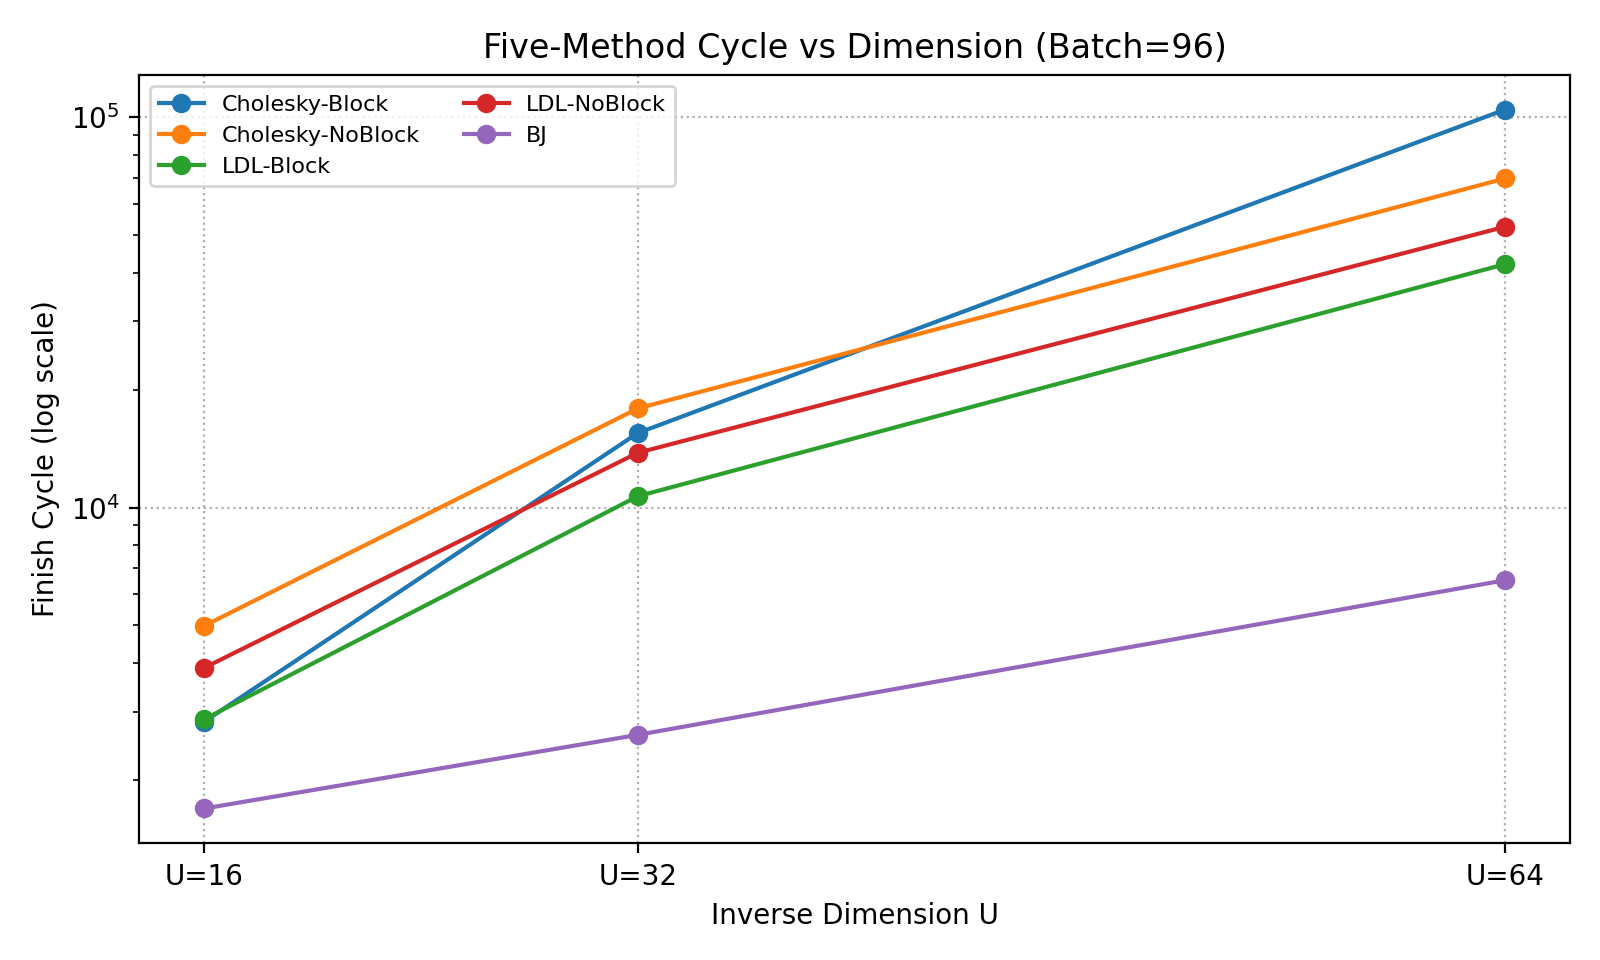
\includegraphics[width=\textwidth]{
                five_methods_cycle_vs_dimension_log.png
            }
            \caption{五算法周期-维度对比（对数坐标）}
        \end{subfigure}
        \begin{subfigure}
            {0.48\textwidth}
            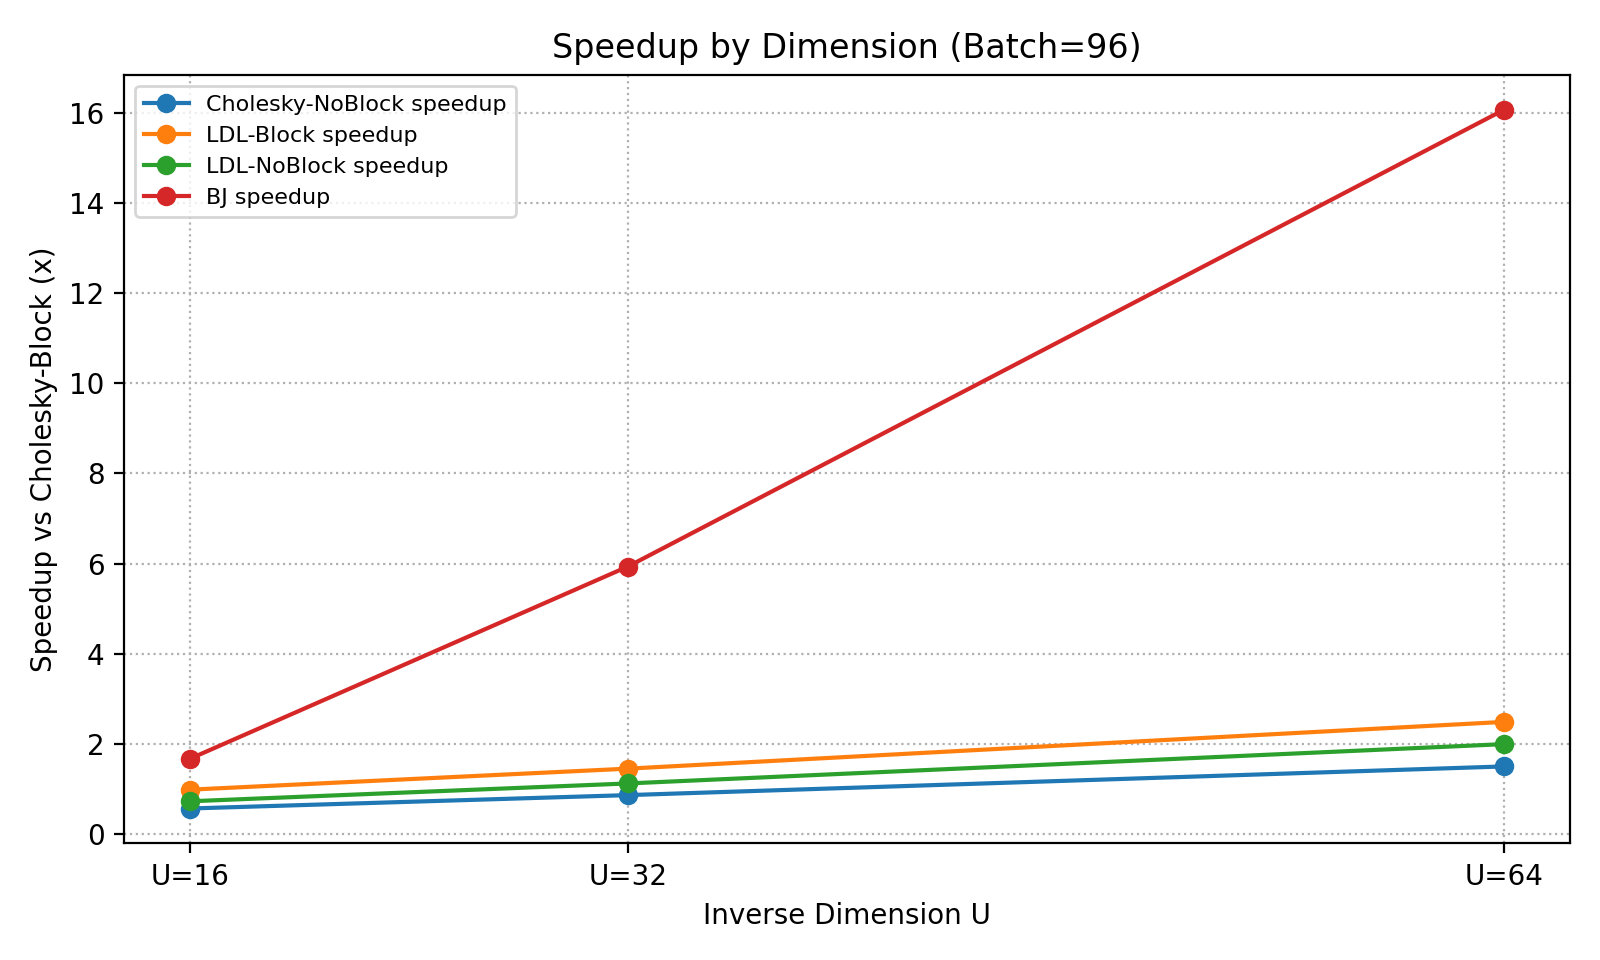
\includegraphics[width=\textwidth]{
                five_methods_speedup_vs_chol_block.png
            }
            \caption{相对 Cholesky-Block 的加速比}
        \end{subfigure}
        \caption{六算法周期与加速比可视化}
        \label{fig:five-cycle-speedup}
    \end{figure}

    \textbf{加速比的物理解释}：BRI 通过”预条件器复用 + 迭代链条可调度”将关键路径集中在规则的
    GEMM 上，同时大幅减少了 Cholesky/LDL 路径中不可并行的串行标量节点（\texttt{SQRT/DIV}）。$U$
    越大，标量节点的累积效应越显著，BRI 的相对优势越突出。

    \subsubsection{静态指令级指标对比}

    各算法在 NPU 上的计算复杂度不仅取决于 FLOPs，更取决于每条指令所映射的\textbf{流水线类型}。在
    Ascend 910B 上，三种流水线的单次操作延迟与并行能力截然不同：

    \begin{itemize}
        \item \textbf{Cube Pipeline}（GEMM\_PRELOAD/GEMM）：$16\times16\times16$
            脉动阵列，单条指令 32 周期（全尺寸），支持多核并行。

        \item \textbf{Vector Pipeline}（ADD/MUL/MAC/DIV）：2048-bit SIMD，单拍处理
            128 个 FP16 元素，延迟 1 周期。

        \item \textbf{Scalar Pipeline}（SCALAR\_ADD/MUL/DIV/SQRT）：单发射，同一时刻只能执行一条
            Scalar 指令，固定延迟（\texttt{div\_latency}、\texttt{scalar\_sqrt\_latency}
            等）。
    \end{itemize}

    六种求逆实现的 FLOPs 与指令类型映射如下：

    \begin{table}[H]
        \centering
        \caption{六算法 NPU 操作复杂度对比（$U$ 为矩阵维度，$L$ 为 BRI
        迭代层数，$K$ 为 NS 迭代次数）}
        \label{tab:five-op-complexity}
        \begin{tabular}{l c c c}
            \toprule \textbf{算法}      & \textbf{总 FLOPs}   & \textbf{关键流水线瓶颈}              & \textbf{Scalar 串行指令}                               \\
            \midrule Cholesky-NoBlock & $\frac{4}{3}U^{3}$ & Scalar SQRT/DIV 逐列串行          & $U \times$ SQRT + $O(U^{2}) \times$ DIV            \\
            Cholesky-Block ($B=2$)    & $\frac{4}{3}U^{3}$ & Scalar SQRT/DIV + 微小 GEMM 碎片化 & $\frac{U}{2}\times$ SQRT + $O(U^{2}/B) \times$ DIV \\
            LDL-NoBlock               & $\frac{5}{3}U^{3}$ & Vector MUL 为主，无 SQRT          & 0 SQRT，$O(U^{2}) \times$ MUL（Vector）               \\
            LDL-Block ($B=2$, packed) & $\frac{5}{3}U^{3}$ & Cube GEMM 粒度提升至 $16\times16$  & 0 SQRT                                             \\
            Block-Richardson ($B=U$)  & $O(LU^{3})$        & Cube GEMM 全部对齐基本块尺寸           & 仅预条件器阶段                                            \\
            Newton-Schulz ($K$)       & $O(KN^{3})$        & 每轮 $2\times$ Cube GEMM（全矩阵）   & 无 Scalar 依赖                                        \\
            \bottomrule
        \end{tabular}
    \end{table}

    几点关键观察：

    \begin{enumerate}
        \item \textbf{Scalar 指令是 NPU 周期瓶颈的核心}。Cholesky-NoBlock 每列需要
            1 次 \texttt{SQRT} + $U-1$ 次 \texttt{DIV}，全部在单发射 Scalar
            Pipeline 上串行执行。对于 $U=64$，这意味 64 次 SQRT 完全无法与 Cube/Vector
            重叠。

        \item \textbf{LDL 消除 SQRT 的收益}。LDL 将 Cholesky 中的 $U^{2}/2$ 次 SQRT
            替换为 $U^{2}$ 次额外 MUL。虽然 MUL 数量增加，但 MUL 走 Vector Pipeline（128
            元素/拍），$\lceil U^{2}/128\rceil$ 周期即可完成，而 SQRT 走 Scalar
            Pipeline 需要 $U\times$\texttt{scalar\_sqrt\_latency} 周期。

        \item \textbf{LDL 拼接降低 Cube 指令数}。$2\times2\rightarrow16\times16$
            拼接将 LDL-Block 的 Cube 指令数从 $O(U^{3})$ 降至 $O(U^{2})$，因为 8
            组 $2\times2$ 的独立 GEMM 合并为单条 $16\times16$ GEMM。

        \item \textbf{BRI 的关键路径最短}。BRI 的迭代主体仅含 $L$ 条 GEMM（$B\ll
            U$
            时通常 $L=3$--$4$ 即收敛），且 GEMM 全部对齐 Cube 基本块尺寸，Cube 利用率达
            60\%（六算法最高）。无任何 Scalar 串行依赖。
    \end{enumerate}

    \begin{table}[H]
        \centering
        \caption{Cholesky vs LDL 指令事件分布对比（24 核全量，$U=16$，$B=2$）}
        \label{tab:five-inst-stats}
        \begin{tabular}{l r r r r}
            \toprule \textbf{事件类型}            & \textbf{Chol-Block} & \textbf{Chol-NoBlock} & \textbf{LDL-Block} & \textbf{LDL-NoBlock} \\
            \midrule Cube（GEMM\_PRELOAD/GEMM） & 19,008              & —                     & 4,896              & 8,064                \\
            Vector（ADD/MUL/MAC）               & 8,832               & —                     & 6,912              & 8,064                \\
            Scalar（SQRT/DIV/MUL）              & 1,536               & —                     & 768                & 1,536                \\
            MTE2（搬运入）                         & 3,840               & 3,840                 & 3,840              & 3,840                \\
            MTE3（搬运出）                         & 768                 & 768                   & 768                & 768                  \\
            PIPE\_BARRIER                     & 1,824               & 672                   & 2,688              & 1,344                \\
            \midrule \textbf{总事件数}            & \textbf{32,448}     & —                     & \textbf{16,416}    & \textbf{20,160}      \\
            \bottomrule
        \end{tabular}
    \end{table}

    该表直观解释了 Cycle 排名差异：LDL-Block 通过拼接将 Cube 指令数从 19,008 压缩至
    4,896（$-$74\%），同时 Scalar 指令从 1,536 减半至 768（$-$50\%）。Cube 指令的减少意味着脉动阵列的发射队列压力下降，而
    Scalar 指令的减半直接缩短了单发射通道上的串行阻塞时间。LDL-Block 的 barrier 事件（2,688）虽高于
    Cholesky-Block（1,824），但 barrier 仅占 1 向量周期，其对总周期的影响远小于 Cube/Scalar
    指令的压缩收益。

    \subsubsection{精度验证指标对比}

    \begin{table}[H]
        \centering
        \caption{六算法全 SNR SE 对比（64QAM，Batch=96，$U=16$）}
        \begin{tabular}{c c c c c c}
            \toprule SNR(dB) & Chol-Block & Chol-NoBlock & LDL-Block & LDL-NoBlock & BRI    \\
            \midrule 0       & 31.799     & 31.799       & 31.798    & 31.798      & 31.800 \\
            5                & 55.096     & 55.096       & 55.097    & 55.097      & 55.100 \\
            10               & 80.251     & 80.251       & 80.251    & 80.252      & 80.251 \\
            15               & 96.000     & 96.000       & 96.000    & 96.000      & 96.000 \\
            20               & 96.000     & 96.000       & 96.000    & 96.000      & 96.000 \\
            25               & 96.000     & 96.000       & 96.000    & 96.000      & 96.000 \\
            30               & 96.000     & 96.000       & 96.000    & 96.000      & 96.000 \\
            \bottomrule
        \end{tabular}
    \end{table}

    \begin{table}[H]
        \centering
        \caption{六算法全 SNR SE 对比（64QAM，Batch=96，$U=32$）}
        \begin{tabular}{c c c c c c}
            \toprule SNR(dB) & Chol-Block & Chol-NoBlock & LDL-Block & LDL-NoBlock & BRI     \\
            \midrule 0       & 63.938     & 63.938       & 63.939    & 63.939      & 63.938  \\
            5                & 109.109    & 109.109      & 109.108   & 109.109     & 109.108 \\
            10               & 159.278    & 159.278      & 159.277   & 159.277     & 159.273 \\
            15               & 192.000    & 192.000      & 192.000   & 192.000     & 192.000 \\
            20               & 192.000    & 192.000      & 192.000   & 192.000     & 192.000 \\
            25               & 192.000    & 192.000      & 192.000   & 192.000     & 192.000 \\
            30               & 192.000    & 192.000      & 192.000   & 192.000     & 192.000 \\
            \bottomrule
        \end{tabular}
    \end{table}

    \begin{table}[H]
        \centering
        \caption{六算法全 SNR SE 对比（64QAM，Batch=96，$U=64$）}
        \begin{tabular}{c c c c c c}
            \toprule SNR(dB) & Chol-Block & Chol-NoBlock & LDL-Block & LDL-NoBlock & BRI     \\
            \midrule 0       & 128.223    & 128.223      & 128.222   & 128.221     & 128.210 \\
            5                & 217.551    & 217.551      & 217.551   & 217.552     & 217.533 \\
            10               & 317.929    & 317.929      & 317.931   & 317.932     & 317.889 \\
            15               & 384.000    & 384.000      & 384.000   & 384.000     & 384.000 \\
            20               & 384.000    & 384.000      & 384.000   & 384.000     & 384.000 \\
            25               & 384.000    & 384.000      & 384.000   & 384.000     & 384.000 \\
            30               & 384.000    & 384.000      & 384.000   & 384.000     & 384.000 \\
            \bottomrule
        \end{tabular}
    \end{table}

    注：64QAM 理论 SE 上限为 $U\times6$ bps/Hz（$U=16\rightarrow96$，$U=32\rightarrow
    192$，$U=64\rightarrow384$）。所有方法在 SNR$\geq15$ dB 后均达到饱和上限。

    \begin{figure}[H]
        \centering
        \begin{subfigure}
            {0.32\textwidth}
            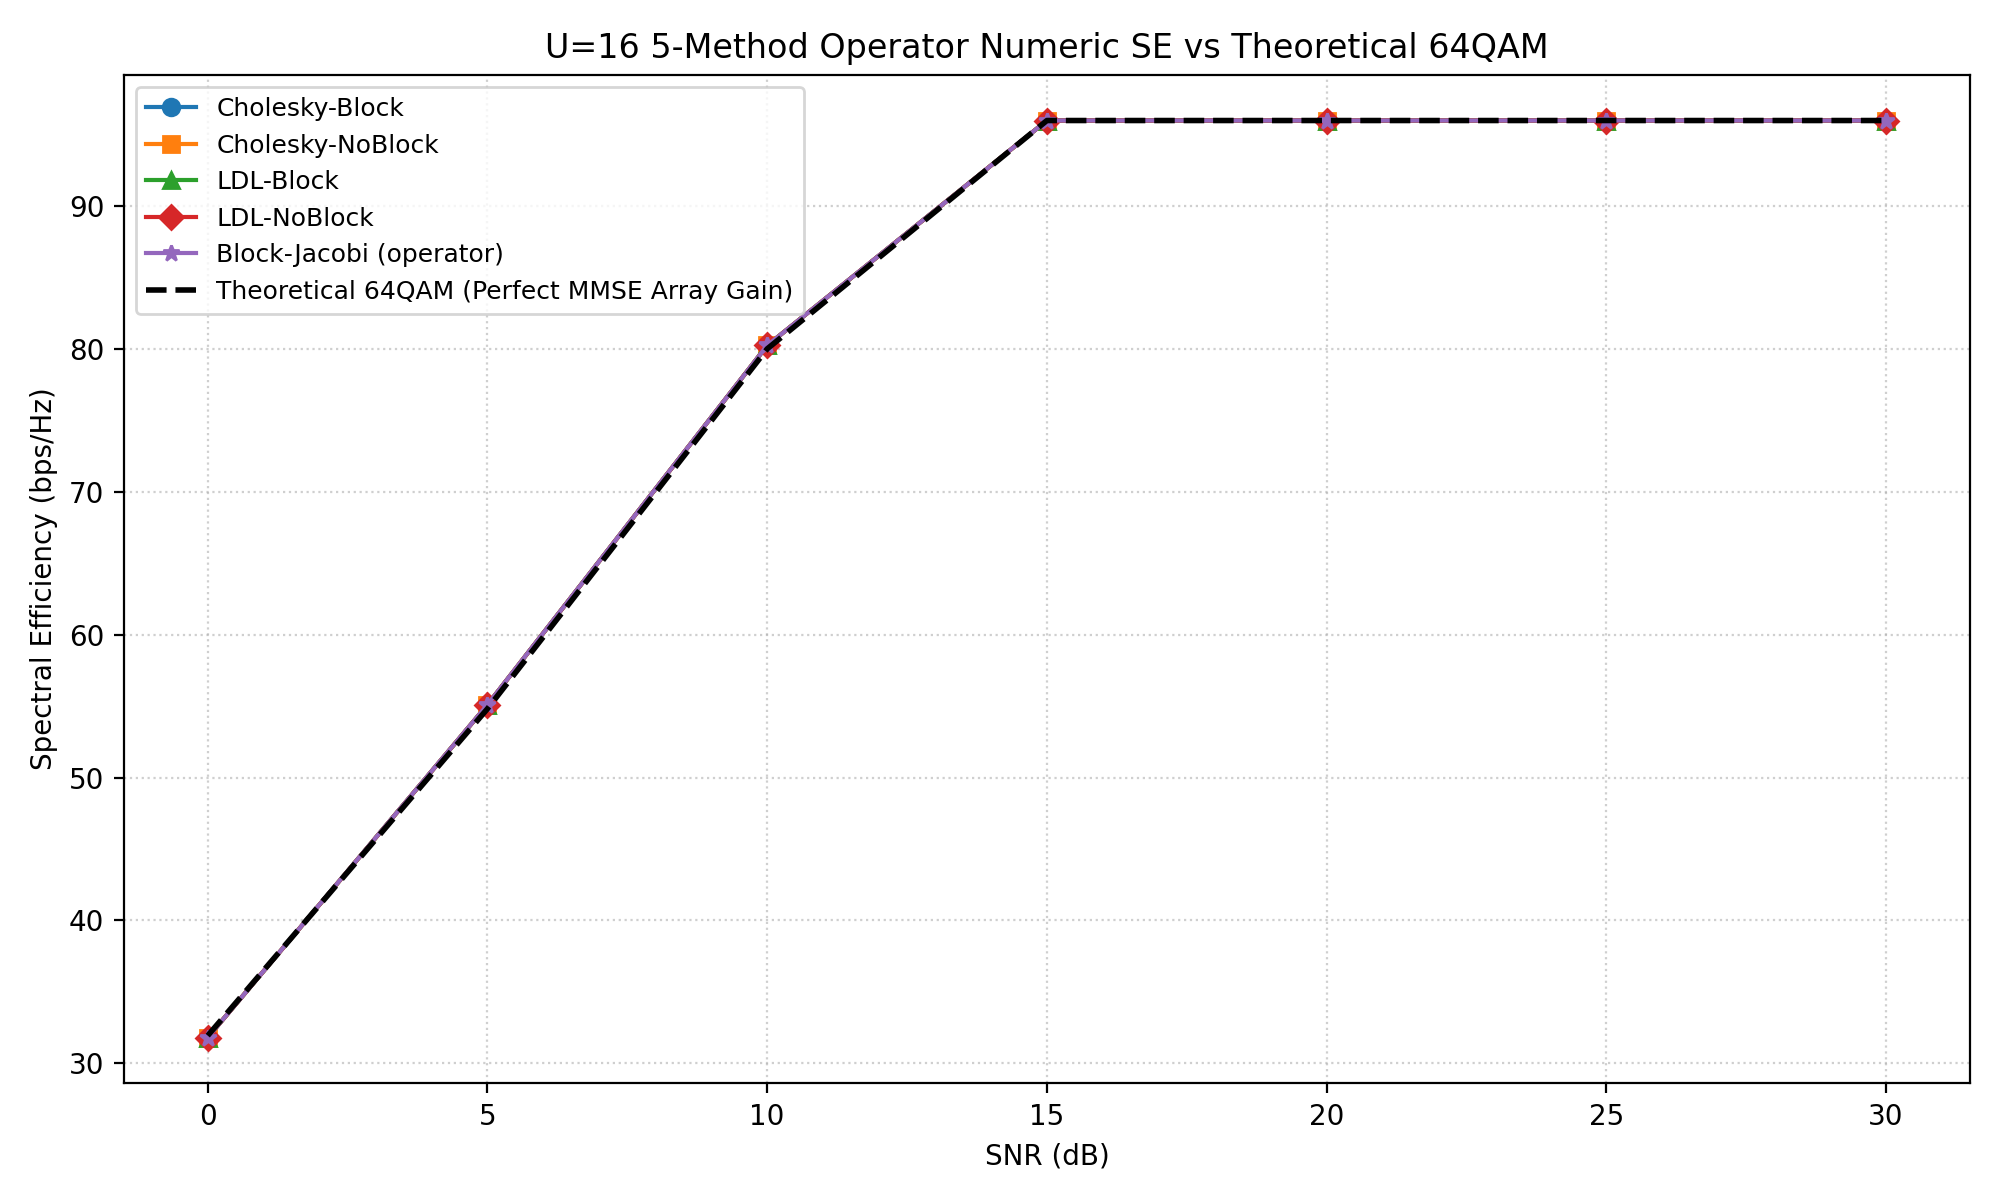
\includegraphics[width=\textwidth]{five_methods_se_u16.png}
            \caption{$U=16$}
        \end{subfigure}
        \begin{subfigure}
            {0.32\textwidth}
            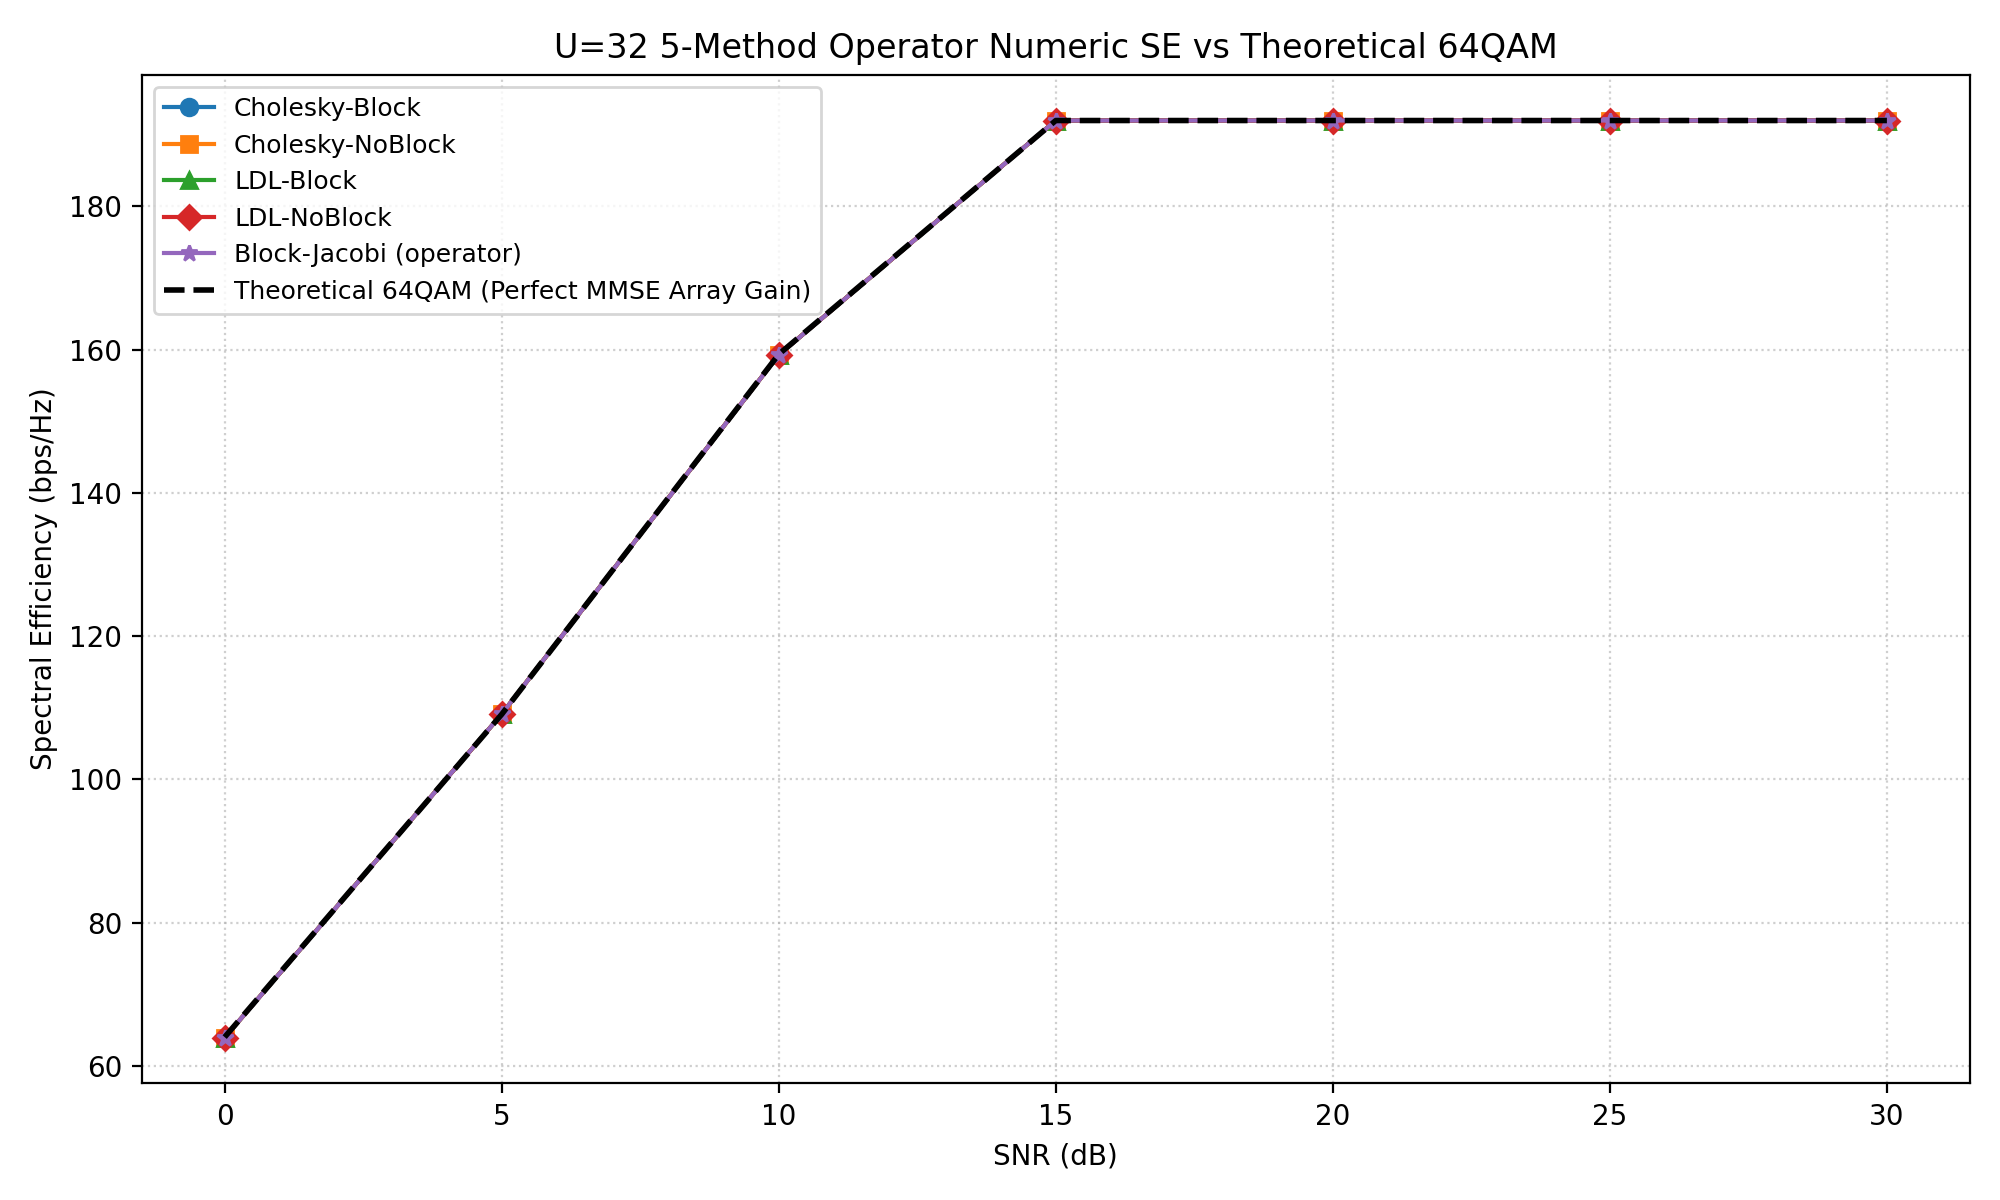
\includegraphics[width=\textwidth]{five_methods_se_u32.png}
            \caption{$U=32$}
        \end{subfigure}
        \begin{subfigure}
            {0.32\textwidth}
            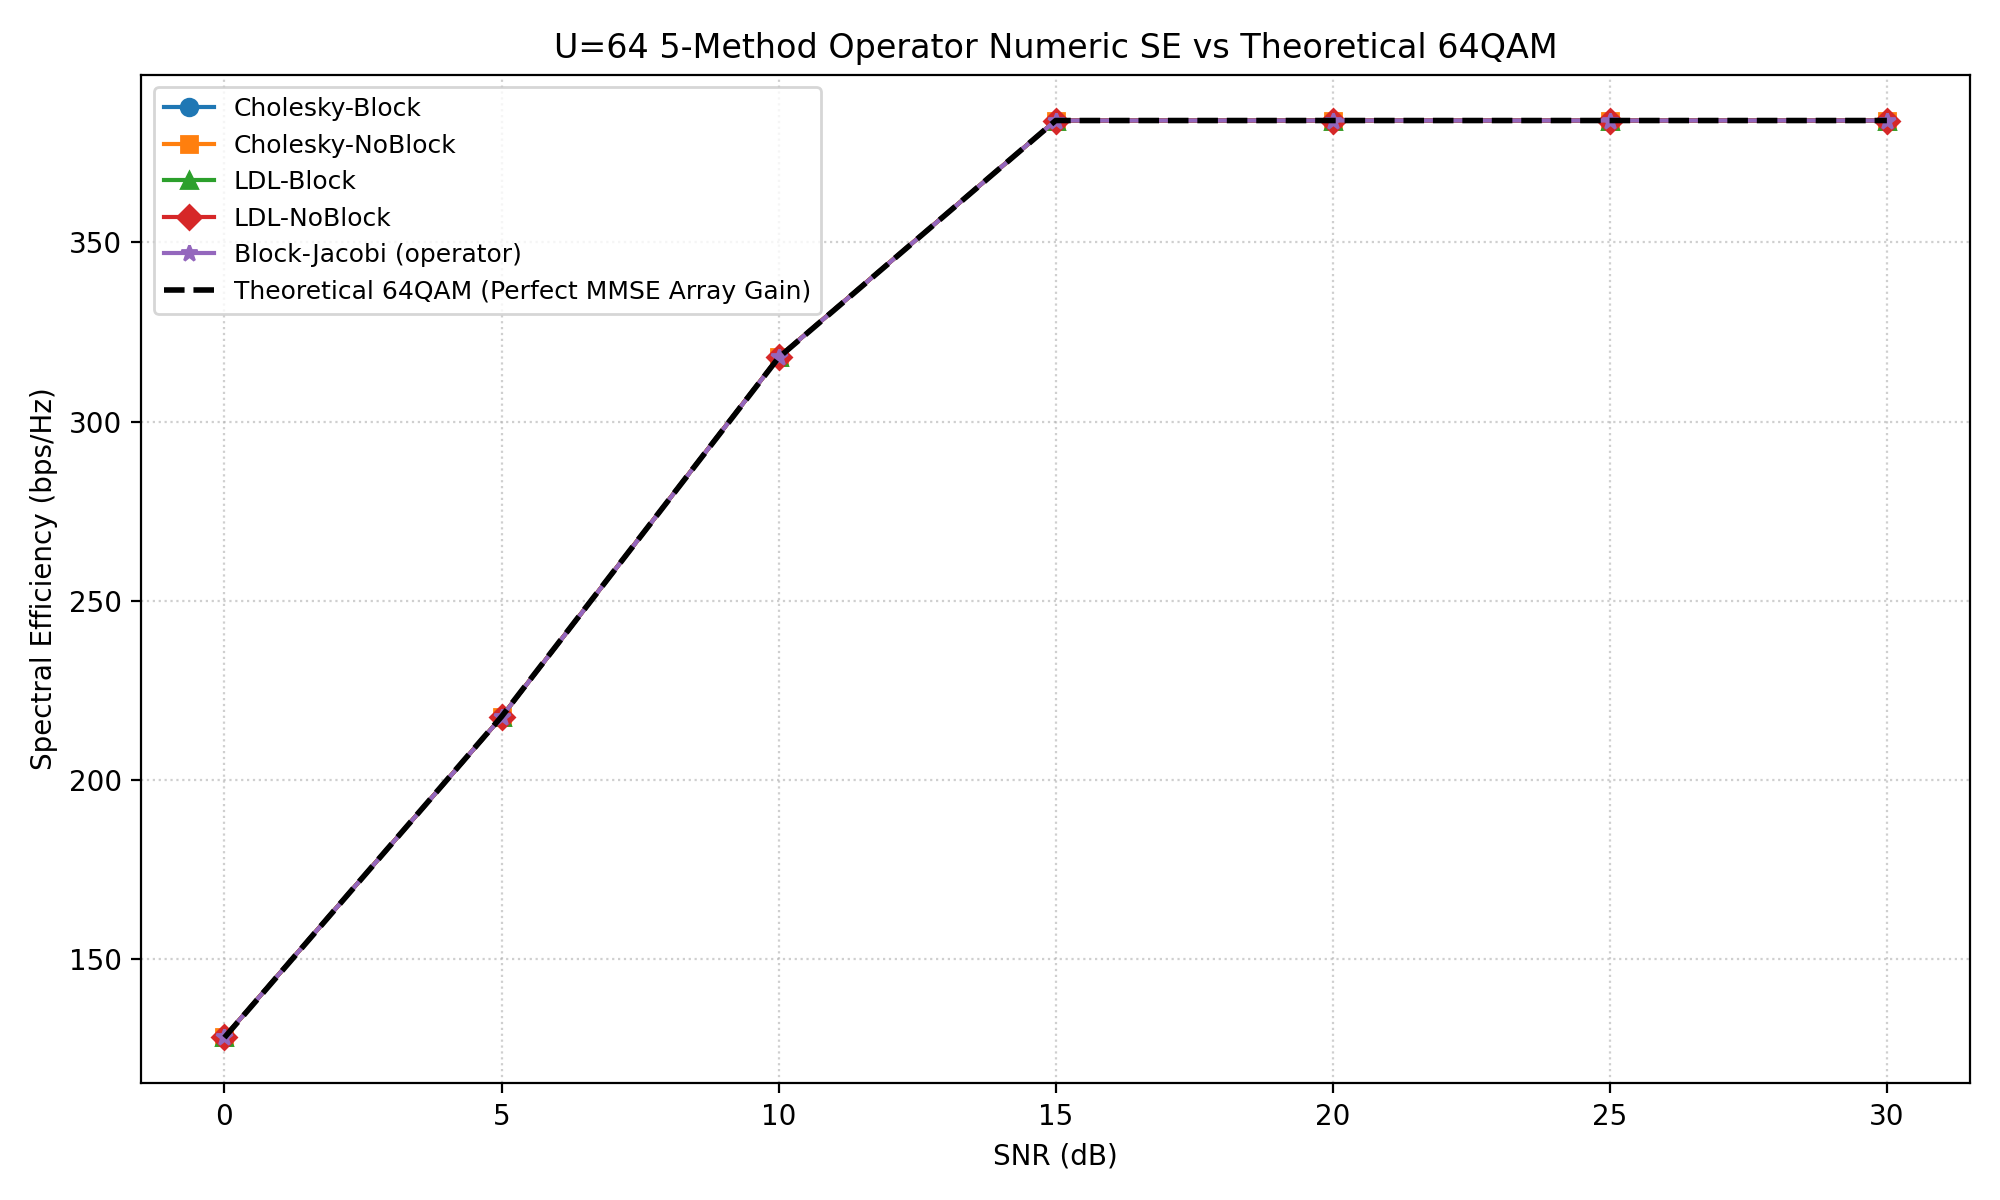
\includegraphics[width=\textwidth]{five_methods_se_u64.png}
            \caption{$U=64$}
        \end{subfigure}
        \caption{六算法 SE-SNR 对比（64QAM，虚线为理论容量上限 $U\times6$ bps/Hz）}
        \label{fig:five-se}
    \end{figure}

    由于 Cholesky 与 LDL 四种实现均为精确求逆，其 SE 曲线在数值上完全一致（差异 $\pm
    0.003$ 以内），不再逐一展开。图~\ref{fig:nonbri-se-grid} 展示了四种精确求逆算法在三个维度下的
    SE-SNR 曲线（为完整起见，各算法独立绘图）。

    \begin{figure}[H]
        \centering
        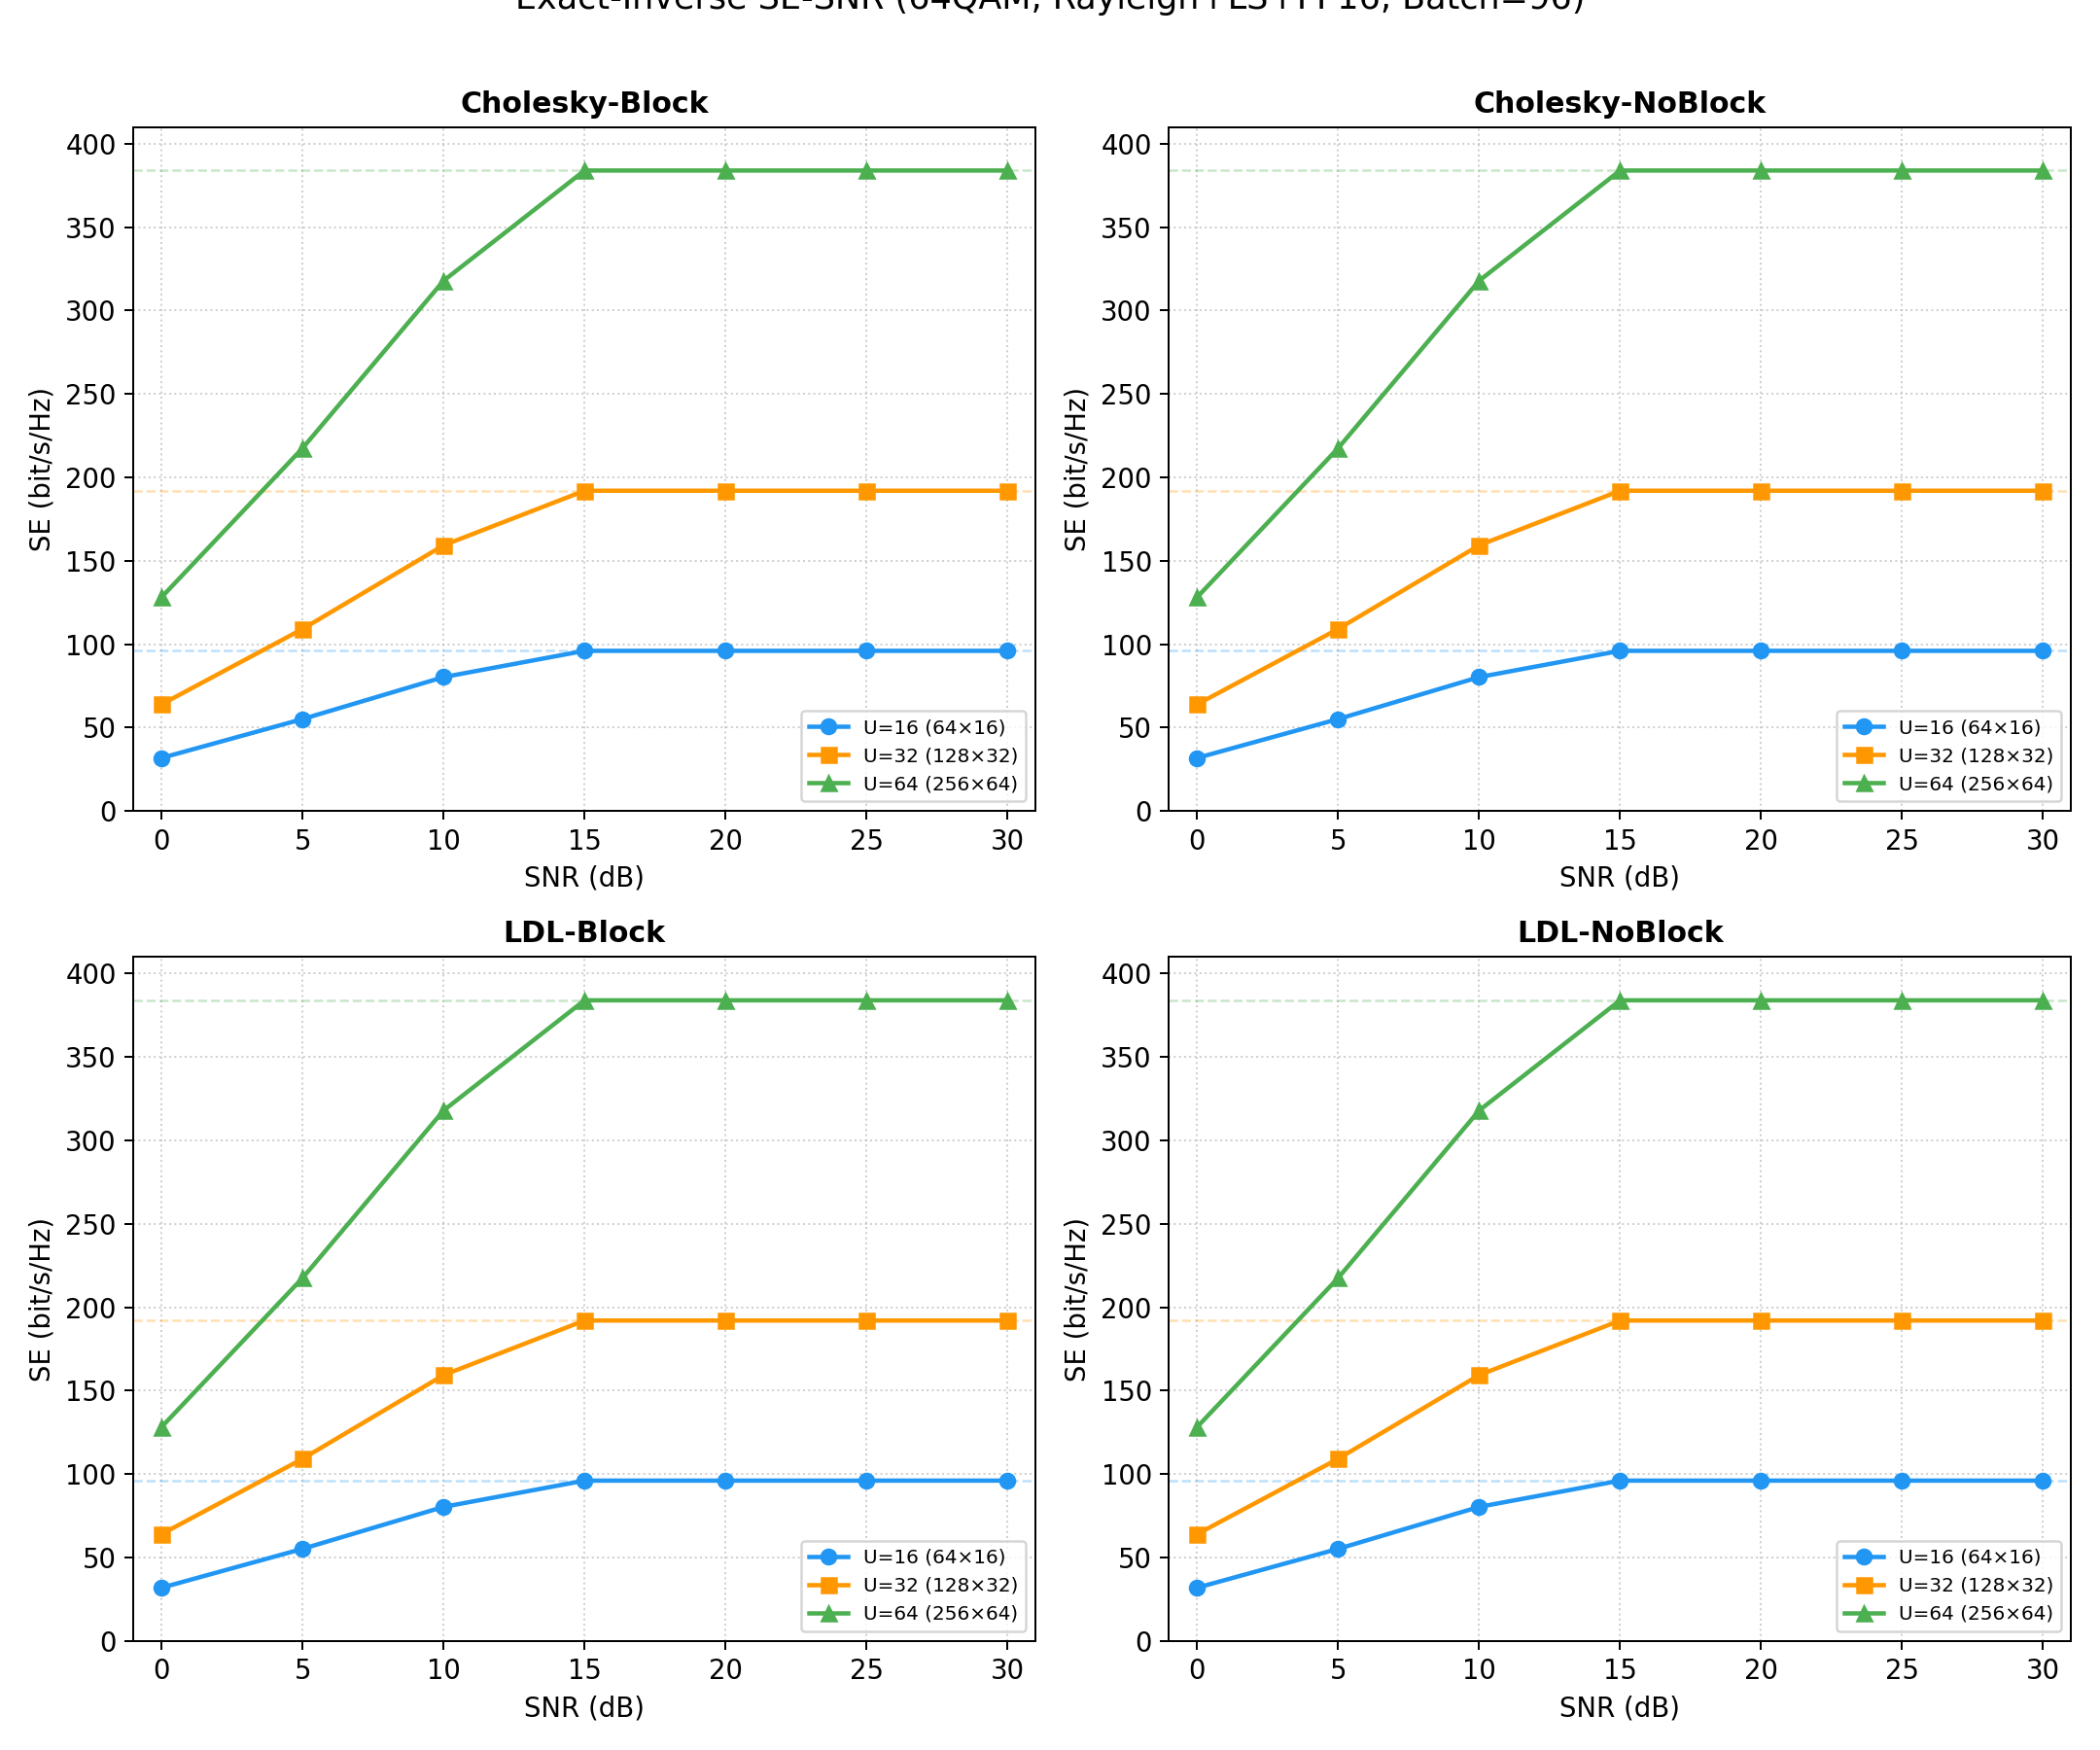
\includegraphics[width=\textwidth]{nonbri_se_grid.png}
        \caption{四种精确求逆算法的 SE-SNR 曲线（64QAM, Rayleigh+LS+FP16, Batch=96；虚线为理论容量上限）}
        \label{fig:nonbri-se-grid}
    \end{figure}

    关键发现：
    \begin{itemize}
        \item \textbf{Cholesky/LDL 四种实现 SE 几乎完全重合}（差异在 $\pm0.003$ 以内），印证了这些直接法的数值等价性。

        \item \textbf{Block-Richardson 的 SE 略低于直接法}，但差距极小（$U=16$
            时差约 0.39；$U=64$ 时差约 1.00），且随 SNR 升高差距缩小，在饱和区（$\geq
            15$
            dB）完全追上。

        \item \textbf{所有方法在 SNR$\geq15$ dB 后均达到 64QAM 的理论容量上限}，说明五种算法在
            64QAM 调制下的数值精度均可靠。

        \item BRI 是“降周期”的方法而非“提升 SE”的方法：它在几乎不牺牲精度（低 SNR
            差距 $<1.5\%$）的前提下，用迭代的计算量换取显著更优的硬件执行效率。
    \end{itemize}

    \textbf{核心利用率对比。}

    来自 \texttt{analyze\_pipeline\_parallelism.py} 的 Core0 流水线活跃占比（$U=1
    6$ 口径，各单元活跃周期数占 Span 的比例，多单元可并行重叠）：

    \begin{table}[H]
        \centering
        \caption{六算法 Core0 流水线活跃占比（\%，各单元活跃周期数占 Span
        的比例，可并行叠加）}
        \begin{tabular}{l c c c c c}
            \toprule \textbf{指标} & Chol-Block & Chol-NoBlock & LDL-Block      & LDL-NoBlock & BRI              \\
            \midrule Cube（脉动阵列）  & 6.83       & 3.87         & \textbf{32.67} & 2.89        & \textbf{59.81}   \\
            Vector（向量）           & 30.73      & 31.95        & 35.46          & 47.37       & 7.20             \\
            Scalar（标量）           & 40.97      & 34.86        & 5.65           & 8.26        & 22.36            \\
            MTE2（搬运入）            & 7.11       & 4.70         & 8.62           & 6.30        & 12.73            \\
            MTE3（搬运出）            & 5.19       & 2.70         & 2.12           & 1.55        & 5.65             \\
            Wait（依赖等待）           & 6.26       & 3.79         & \textbf{26.25} & 2.81        & 16.83            \\
            \midrule 平均流水线并行度    & 0.91       & 0.78         & 0.85           & 0.66        & \textbf{1.08}    \\
            流水线重叠率($\ge$2单元)     & 16.57\%    & 6.88\%       & 13.71\%        & 7.59\%      & \textbf{20.62\%} \\
            \bottomrule
        \end{tabular}
    \end{table}

    LDL-Block 的 Cube 活跃占比（32.67\%）远高于其他 Cholesky 实现（2.89--6.83\%），直接验证了
    $2\times2\rightarrow16\times16$ 拼接优化的效果——拼接使 GEMM 粒度对齐 Cube
    基本块，减少了脉动阵列的空转。LDL-Block 的 Wait 占比也最高（26.25\%），说明拼接带来了更积极的并行发射，同时暴露了更多依赖等待窗口。Block-Richardson
    的 Cube 活跃占比最高（59.81\%），印证了其以 GEMM
    为主的计算特征；同时其流水线并行度（1.08）与重叠率（20.62\%）均为五算法最优，说明
    BRI 的 GEMM 流水线与搬运操作实现了最好的重叠。

    \subsubsection{迭代法的算法对比与 BRI 的加速优势}
    \label{sec:ns-vs-bri}

    Newton-Schulz（NS）是矩阵求逆的经典迭代方法，在前节已作为迭代基线进行了完整推导与分析。本节简要对比二者的算法结构差异，完整的收敛分析、SE
    验证和 NPU 实测数据请参见第~\ref{sec:ns-algo} 节（算法三）。

    \textbf{算法结构对比。} NS 与 BRI 的核心差异在于预条件策略：

    \begin{itemize}
        \item \textbf{NS}：$\bm{X}_{k+1}= \bm{X}_{k}(2\bm{I}- \bm{A}\bm{X}_{k})$，二阶收敛。初始猜测
            $\bm{X}_{0}=\bm{I}/\|\bm{A}\|_{2}$ 保证对任意正定矩阵收敛。每轮 2 次完整
            GEMM（$O(N^{3})$）+ 1 次 ADD。不依赖矩阵结构信息。

        \item \textbf{BRI}：$\bm{y}_{k+1}= \bm{y}_{k}+ \omega_{k}(\bm{I}- \bm{M}\bm
            {y}_{k})$，线性收敛 + Chebyshev 加速。预条件器 $\bm{M}= \operatorname{blockdiag}
            (\bm{A}_{11},\dots,\bm{A}_{bb})$ 利用 MIMO 信道的对角块主导性质，每轮
            1 次块对角 GEMM（$O(B N^{2})$）+ 1 次 AXPY。
    \end{itemize}

    \textbf{单次迭代计算量对比：}

    \begin{table}[H]
        \centering
        \caption{单次迭代浮点操作量对比（$N\times N$ 矩阵，$B$ 为 BRI 分块大小，$K$
        为 NS 迭代次数，$L$ 为 BRI 迭代层数）}
        \begin{tabular}{l c c c}
            \toprule \textbf{操作类型}                            & \textbf{Newton-Schulz ($K$)} & \textbf{Block-Richardson ($L$)} & \textbf{比值}              \\
            \midrule 矩阵乘法（Cube GEMM）                          & $2K N^{3}$                   & $L B N^{2}$                     & $2K N / (L B)$           \\
            逐元素运算（Vector）                                     & $K N^{2}$                    & $2L N^{2}$                      & $K/(2L)$                 \\
            Pipe Barrier                                      & $2K$ 次                       & $L$ 次                           & —                        \\
            \midrule \textbf{典型值（$N{=}32,K{=}8,B{=}2,L{=}4$）} & $\sim 5.2\times 10^{5}$      & $\sim 8.2\times 10^{3}$         & $\mathbf{\sim 64\times}$ \\
            \bottomrule
        \end{tabular}
    \end{table}

    \textbf{核心结论（详见第~\ref{sec:ns-algo} 节）：}
    \begin{enumerate}
        \item SE 实测：NS（$K=8$，$\bm{X}_{0}=\bm{I}/\|\bm{A}\|_{2}$）在所有维度均达到容量
            SE，$\bar{\varepsilon}_{\text{rel}}$ $=3.76\times 10^{-4}$；BRI（$B=2,L=3$--$4$）同样达到容量
            SE。两种方法的 SE 最终值完全一致。

        \item NPU 周期：BRI 在所有维度下均快于 NS（$N=16$: $1.95\times$, $N=32$:
            $5.79\times$, $N=64$: $6.27\times$）。NS 的 $O(K\cdot N^{3})$ 全矩阵
            GEMM 量级随维度立方增长，BRI 的 $O(L\cdot B\cdot N^{2})$ 块对角稀疏
            GEMM 仅随维度平方增长。

        \item NS 的价值：算法实现简单（无需预条件器构建、无需分块参数选择），对信道结构无假设（对角占优和非对角占优场景均适用），适合作为快速原型验证工具和
            BRI 失效场景（如极端相关信道导致块对角预条件器退化）的备选方案。
    \end{enumerate}
    % =================================================================================


    \subsection{本章小结}

    本章从统一的 MMSE 框架出发，系统给出了 Cholesky（No-Block/Block）、LDL（No-Block/Block）、Block-Richardson
    和 Newton-Schulz 六种求逆实现的完整推导、NPU 指令映射（Cube/Vector/Scalar）和分步骤优化过程。

    核心发现总结如下：

    \begin{enumerate}
        \item \textbf{算法有效性}：Cholesky/LDL 四种直接法在 SE 上几乎完全重合（差异
            $<0.003$），Block-Richardson 与 Newton-Schulz 的 SE
            略低但保持同阶（低 SNR 差距 $<1.5\%$），且在高 SNR 饱和区完全追上。

        \item \textbf{周期优势}：Block-Richardson 在所有维度下均为周期最优，优势随
            $U$ 增大呈指数级放大（$1.67\times\rightarrow5.93\times\rightarrow16.0
            7\times$）。Newton-Schulz（$K=8$，$\bm{X}_{0}=\bm{I}/\|\bm{A}\|_{2}$）在所有维度下均位列第三（$4
            ,304/30,561/100,029$），其 $O(K\cdot N^{3})$ 全矩阵 GEMM 量级无法与 BRI
            的 $O(L\cdot B\cdot N^{2})$ 块对角稀疏 GEMM 竞争。

        \item \textbf{NPU 优化关键}：每种算法都存在其特定的 NPU 瓶颈——Cholesky 的
            \texttt{SQRT/DIV} 串行依赖（Scalar）、LDL 的微小 GEMM 碎片化（Cube
            利用率低）、BRI 的 \texttt{BY\_*} 重复 preload（Cube）、NS 的每轮 $2\times$
            全矩阵 GEMM（Cube 量级 $O(N^{3})$）。针对性地做“拼接对齐 Cube
            尺寸”“融合发射与 Kernel 合并”“barrier
            密度调优”等结构改造，收益远超盲目增加算力。

        \item \textbf{流水线映射规律}：Cube（GEMM）是吞吐最高的单元但需要大粒度 Tile
            对齐 $16\times16\times16$；Vector（ADD/MUL/MAC）适合逐元素操作但需避免阻塞
            Scalar；Scalar（SQRT/DIV）是单发射串行通道，是 Cholesky/LDL
            的绝对瓶颈。将操作从 Scalar 转移到 Cube 或 Vector 是 NPU
            优化的核心策略。

        \item \textbf{AI 优化的方法论}：以 \texttt{skill} 为统一评测平台，在 SE
            不回退的硬约束下，通过瓶颈归因 $\rightarrow$ 调度改造 $\rightarrow$
            离散搜索的标准化路径，实现了 BRI 从基线 2550 到 P2 最优 1893 的
            $25.76\%$ 周期压缩，且全链路可审计、可复现。
    \end{enumerate}

    % =================================================================================

    \section{仿真环境与底层基础设施 (Asim)}
    \label{sec:asim-infra}

    为从芯片微架构级别对通信算法进行时钟周期 (Cycle) 精度和数值误差 (SE)
    的全方位度量，本团队主导了对底层仿真器的重构工作。本章围绕三个部分展开：\textbf{仿真平台搭建}（Asim
    架构设计、硬件建模、周期模型、指令集体系）、\textbf{仿真器运行流程}（自动化评测流水线、并发调度修复、评测实验管理）、以及\textbf{仿真器验证方法}（周期精度验证、UOBS
    黑盒评估框架）。图~\ref{fig:asim-chapter-overview} 首先给出了 Asim 内部维护的硬件抽象层级和周期推进主流程。

    \subsection{仿真平台架构}

    为从芯片微架构级别对通信算法进行时钟周期 (Cycle) 精度和数值误差 (SE) 的全方位度量，本团队主导了对底层仿真器的重构工作。以下各节依次阐述
    Asim 的架构设计、硬件建模、周期模型和指令集体系。本章后续两节分别覆盖仿真器运行流程和仿真器验证方法。图~\ref{fig:asim-chapter-overview}
    给出了 Asim 在周期推进过程中维护的核心抽象层级：模型和算子首先被展开为 Tile 与指令流，随后由调度器发射到 Core 内部的
    \texttt{LD/ST/EX} 队列；访存请求经片上互连进入片外 DRAM，而计算指令根据 opcode 被路由到 Cube、Vector 或 Scalar
    流水线，并通过 SPAD/ACCUM 的命中状态维护数据依赖。

    \begin{figure}[H]
        \centering
        \resizebox{0.98\textwidth}{!}{%
        \begin{tikzpicture}[
            font=\small,
            >=Latex,
            block/.style={draw, rounded corners=2pt, align=center, inner sep=6pt, minimum height=1.05cm, text width=3.0cm},
            stage/.style={block, fill=cyan!10},
            core/.style={block, fill=blue!7},
            state/.style={block, fill=orange!10},
            mem/.style={block, fill=red!8},
            note/.style={align=center, font=\scriptsize, text=black!70, text width=4.2cm},
            arr/.style={-{Latex[length=2.2mm]}, line width=0.6pt, black!70},
            barr/.style={{Latex[length=2.2mm]}-{Latex[length=2.2mm]}, line width=0.6pt, black!70},
            darr/.style={-{Latex[length=2.2mm]}, dashed, line width=0.55pt, black!55}
        ]
            % ====== Control path ======
            \node[stage] (model) at (0, 4.25) {Model / Operation\\张量图与算子语义};
            \node[stage] (tile) at (4.1, 4.25) {Tile / Instruction\\算子下沉为指令序列};
            \node[stage] (sched) at (8.2, 4.25) {Scheduler\\按 Core 发射 Tile};
            \node[stage] (cycle) at (12.3, 4.25) {Cycle Driver\\推进 Core / ICNT / DRAM};

            \draw[arr] (model) -- (tile);
            \draw[arr] (tile) -- (sched);
            \draw[arr] (sched) -- (cycle);
            \node[note, text width=7.2cm] at (6.15, 5.05) {控制流：决定 Tile 生成、调度与三时钟域推进顺序};

            % ====== Core abstraction ======
            \node[core, minimum height=1.35cm] (queues) at (0, 1.75)
                {Instruction Queues\\\texttt{LD: MOVIN}\\\texttt{EX: GEMM/Vector/Scalar}\\\texttt{ST: MOVOUT}};
            \node[state, minimum height=1.35cm] (scratch) at (4.1, 1.75)
                {On-chip State\\SPAD / ACCUM SPAD\\地址命中与数据依赖};
            \node[core, minimum height=1.35cm] (pipes) at (8.2, 1.75)
                {Execution Pipelines\\Cube / Vector / Scalar\\按 opcode 计算周期};
            \node[stage, minimum height=1.35cm] (output) at (12.3, 1.75)
                {Simulation Output\\cycle stats / TPS\\trace.csv / JSON};

            \node[draw, rounded corners=4pt, dashed, inner sep=10pt,
                  fit=(queues)(scratch)(pipes),
                  label={[font=\bfseries]above:Core 内部维护的抽象状态}]
                  (corebox) {};

            \draw[arr] (cycle.south) -- ++(0,-0.6) -| (queues.north);
            \draw[arr] (queues) -- (scratch);
            \draw[arr] (scratch) -- (pipes);
            \draw[arr] (pipes) -- (output);
            \draw[darr] (pipes.south) -- ++(0,-0.55) -| (scratch.south);

            % ====== Memory path ======
            \node[mem] (icnt) at (4.1, -1.25) {ICNT / NoC\\SimpleInterconnect / Booksim2};
            \node[mem] (dram) at (8.2, -1.25) {Off-chip DRAM\\Ramulator2 HBM2\\固定粒度 memory request};

            \draw[barr] (scratch.south) -- (icnt.north);
            \draw[barr] (icnt) -- (dram);

            \node[note, text width=5.8cm] at (3.0, -2.75)
                {片上执行流：指令队列检查依赖，SPAD/ACCUM 记录占用与命中，执行流水线完成后回填片上状态。};
            \node[note, text width=5.8cm] at (9.3, -2.75)
                {片外访存流：\texttt{MOVIN}/\texttt{MOVOUT} 生成 memory request，经 NoC 与 DRAM 模型决定等待时间。};
        \end{tikzpicture}%
        }
        \caption{Asim 仿真器内部抽象层级与周期推进流程：模型层输出 Tile 与指令流，调度器将 Tile 发射到 Core；Core 通过 \texttt{LD/ST/EX} 队列、SPAD/ACCUM 片上存储和 Cube/Vector/Scalar 流水线维护指令依赖与执行时延；访存请求经 ICNT/NoC 进入片外 DRAM，最终共同形成周期统计、TPS、Timeline 与指令级导出结果。}
        \label{fig:asim-chapter-overview}
    \end{figure}

    该层级关系说明了 Asim 的仿真对象并不是单纯的数学算子，而是由算子下沉得到的硬件指令序列。C++ 时序仿真侧依据
    \texttt{src\_addrs}、SPAD/ACCUM 分配状态和多流水线占用情况决定指令何时可发射；片外访存则被拆分为固定粒度请求，通过
    ICNT/NoC 与 DRAM 模型共同决定实际等待时间。因此，本章后续关于平台搭建、运行流程与验证方法的讨论，都围绕这一“指令
    -- 片上存储 -- 执行流水 -- 片外访存”的闭环展开。

    \subsubsection{Asim 仿真器架构设计}

    \paragraph{Model/Operation 到指令调度流}
    Asim 的前端抽象用于描述“要执行什么计算”。模型层（\texttt{src/models/*}）负责创建 Tensor、组织算子依赖关系，并把完整算法链路拆成若干
    Operation；算子层（\texttt{src/operations/*}）进一步把宏观算子下沉为 Tile
    粒度的指令序列。每个 Tile 内部不再保存高阶数学表达式，而是保存显式的硬件指令，例如
    \texttt{MOVIN}、\texttt{GEMM\_PRELOAD}、\texttt{GEMM}、Vector opcode、Scalar opcode
    与 \texttt{MOVOUT}。这些指令携带源地址、目的地址、数据规模、tile
    形状和依赖地址等字段，构成后端时序仿真的最小输入。

    因此，Model 与 Operation 的职责边界可以概括为：Model 定义张量与算子图，Operation
    定义该算子在硬件上的 tile 化展开方式，Scheduler 则只消费已经生成好的 Tile
    队列。当前调度器按 Layer/Tile/Core 维护生命周期，将就绪 Tile
    发射到对应 Core 的 Tile Queue，并在 Tile 完成后推进后续 Layer。此时，仿真器已经不再关心“这是矩阵求逆还是矩阵乘”，而只关心一串可调度的硬件指令。

    \paragraph{硬件功能模型对指令流的消费}
    Asim 的后端抽象用于描述“这些指令如何在硬件上消耗周期”。每个 Core 内部维护
    Load、Execute、Store 三类指令队列：\texttt{MOVIN} 进入 Load 队列并产生 DRAM
    读请求，\texttt{MOVOUT} 进入 Store 队列并产生 DRAM 写请求，计算类 opcode 进入 Execute
    队列。Execute 队列发射前会检查 \texttt{src\_addrs} 所指向的数据是否已经在 SPAD/ACCUM
    中命中；若操作数尚未由前序 \texttt{MOVIN} 或计算指令填充，则该指令不能发射，从而形成类似
    Scoreboard 的数据相关约束。

    在计算路径上，opcode 决定指令进入哪条执行流水线：\texttt{GEMM} 与
    \texttt{GEMM\_PRELOAD} 进入 Cube Pipeline，向量类指令进入 Vector Pipeline，标量类指令进入
    Scalar Pipeline。各流水线按照配置中的硬件参数计算 \texttt{start\_cycle} 与
    \texttt{finish\_cycle}，指令完成后再更新 SPAD/ACCUM 的占用和命中状态。在访存路径上，
    \texttt{MOVIN}/\texttt{MOVOUT} 生成固定粒度 memory request，经 ICNT/NoC
    传输到片外 DRAM，再由 DRAM 模型返回响应。因此，总周期并不是单条指令延迟的简单相加，而是由片上依赖、流水线占用、NoC
    传输和 DRAM 排队共同决定。

    \paragraph{基于 Ascend 910B 的硬件参数配置}
    Asim 通过 \texttt{configs/ascend\_910b.json} 对类 Ascend 910B
    硬件进行参数化配置，而不是在代码中固定某个单一算子的周期。Operation
    生成的指令只描述“做什么”和“访问哪里”，而表~\ref{tab:ascend910b-onchip-config}
    与表~\ref{tab:ascend910b-memory-config} 中的参数决定这些指令在目标硬件配置下如何消耗周期。

    \begin{table}[H]
        \centering
        \caption{类 Ascend 910B 的片上计算与存储参数配置}
        \label{tab:ascend910b-onchip-config}
        \footnotesize
        \setlength{\tabcolsep}{3pt}
        \renewcommand{\arraystretch}{1.12}
        \begin{tabular}{p{2.4cm} p{3.2cm} p{2.3cm} p{5.4cm}}
            \toprule
            \textbf{类别} & \textbf{配置项} & \textbf{取值} & \textbf{仿真含义} \\
            \midrule
            Core 数量 & \texttt{num\_cores} & 24 &
            创建 24 个同构 \texttt{SystolicWS} Core，Scheduler 将 Tile 发射到这些 Core 的队列。 \\

            Core 时钟 & \texttt{core\_freq} & 1200 MHz &
            决定 Core 侧 \texttt{cycle()} 的时间步长，并参与 TPS 和周期时间换算。 \\

            Core 统计 & \texttt{core\_print\_interval} & 10000 &
            控制 Core 周期统计信息输出间隔。 \\

            Core 类型 & \texttt{core\_type} & \texttt{systolic\_ws} &
            每个 core 均使用 weight-stationary systolic array 执行模型。 \\

            脉动阵列规模 & \texttt{core\_width}/\texttt{core\_height} & $16/16$ &
            用于估计基础 systolic array 吞吐。 \\

            Ascend Cube 模型 & \texttt{enabled}，\texttt{cube\_m/n/k}，\texttt{cube\_base\_latency} & true，$16/16/16$，1 &
            GEMM 按 $16\times16\times16$ 微块计算 block 数，并叠加基础启动延迟。 \\

            片上存储容量 & \texttt{spad\_size}/\texttt{accum\_spad\_size} & 262144 B / 262144 B &
            每核 SPAD 与 ACCUM SPAD 均为 256 KB，用于维护片上地址分配、命中状态和双缓冲。 \\

            SRAM 宽度 & \texttt{sram\_width} & 64 B &
            表征片上 SRAM 访问宽度，也与搬运粒度建模保持一致。 \\

            Vector 宽度 & \texttt{vector\_process\_bit} & 2048 bit &
            Vector Pipeline 每次处理的数据位宽，用于计算向量 opcode 的迭代次数。 \\

            Vector 延迟 & \texttt{add/mul/mac}=1，\texttt{exp/gelu}=2，\texttt{div}=4，\texttt{add\_tree}=2 & cycle &
            不同向量类 opcode 的基础周期参数。 \\

            Scalar 延迟 & \texttt{scalar\_sqrt}=4，\texttt{scalar\_add/mul}=1 & cycle &
            标量流水线上的基础延迟参数，用于建模 SQRT 等串行瓶颈。 \\

            全局 SRAM & \texttt{sram\_size} & 134217728 B &
            配置全局 SRAM 容量为 128 MB，作为整体存储层级参数。 \\
            \bottomrule
        \end{tabular}
    \end{table}

    \begin{table}[H]
        \centering
        \caption{类 Ascend 910B 的片外访存、NoC 与调度参数配置}
        \label{tab:ascend910b-memory-config}
        \footnotesize
        \setlength{\tabcolsep}{3pt}
        \renewcommand{\arraystretch}{1.12}
        \begin{tabular}{p{2.4cm} p{3.2cm} p{2.3cm} p{5.4cm}}
            \toprule
            \textbf{类别} & \textbf{配置项} & \textbf{取值} & \textbf{仿真含义} \\
            \midrule
            DRAM 类型 & \texttt{dram\_type}，\texttt{dram\_config\_path} & \texttt{ramulator2}，HBM2 &
            片外访存由 Ramulator2 HBM2 模型处理，包含通道排队和 DRAM 时序约束。 \\

            DRAM 时钟 & \texttt{dram\_freq} & 1200 MHz &
            决定 DRAM 侧 \texttt{cycle()} 的时间步长。 \\

            DRAM 通道 & \texttt{dram\_channels} & 32 &
            仿真器创建 32 个 DRAM channel；地址通过 \texttt{get\_channel\_id()} 哈希映射到通道。 \\

            访存粒度/对齐 & \texttt{dram\_req\_size} & 64 B &
            每条 \texttt{MemoryAccess} 固定为 64 B；Ramulator2 侧断言 DRAM 地址必须按 64 B 对齐，因此 MOVIN/MOVOUT 会被拆成若干 64 B 请求。 \\

            DRAM 延迟 & \texttt{dram\_latency} & 100 cycle &
            简单 DRAM 模型使用的固定延迟参数；当前 Ramulator2 路径主要由 HBM2 配置和通道排队决定返回时间。 \\

            DRAM 容量/突发 & \texttt{dram\_size}/\texttt{dram\_nbl} & 64 GB / 1 &
            用于带宽估计，峰值带宽按 \texttt{dram\_freq * dram\_channels * dram\_req\_size / dram\_nbl} 计算。 \\

            DRAM 统计 & \texttt{dram\_print\_interval}，\texttt{dram\_bandwidth} & 9600，1200 &
            控制 DRAM 统计输出，并保留名义带宽配置字段。 \\

            NoC 类型 & \texttt{icnt\_type} & \texttt{simple} &
            当前使用 \texttt{SimpleInterconnect} 模型；也保留 Booksim2 配置路径。 \\

            NoC 时钟/延迟 & \texttt{icnt\_freq}/\texttt{icnt\_latency} & 1200 MHz / 1 cycle &
            NoC 每跳注入后至少经历 1 个 ICNT 周期，并在输入队列中按目的节点轮询仲裁。 \\

            NoC 注入端口 & \texttt{icnt\_injection\_ports\_per\_core} & 8 &
            每个 Core 有 8 个注入端口；NoC 节点总数为 $24\times8+32=224$，包括 192 个 Core 侧端口节点和 32 个 DRAM 节点。 \\

            NoC 配置文件 & \texttt{icnt\_config\_path} & booksim2 fly 配置 &
            当 \texttt{icnt\_type} 切换为 Booksim2 时使用；当前 simple 路径主要使用注入端口数和固定延迟。 \\

            数据格式 & \texttt{precision}/\texttt{layout} & 2 B / \texttt{NHWC} &
            默认 FP16 数据宽度为 2 Byte，并使用 NHWC 张量布局。 \\

            调度器 & \texttt{scheduler} & \texttt{simple} &
            使用简单 Layer/Tile 调度策略，将就绪 Tile 分发到 Core。 \\
            \bottomrule
        \end{tabular}
    \end{table}

    由此可见，片上计算参数和片外访存参数共同决定最终周期：Cube/Vector/Scalar
    配置决定计算指令的服务时间，SPAD/ACCUM 状态决定依赖是否满足，64B 对齐的 DRAM 请求粒度、32 个 DRAM channel
    与每 Core 8 个 NoC 注入端口共同决定 \texttt{MOVIN}/\texttt{MOVOUT} 的请求数量、通道分布和排队等待时间。

    关键仿真入口包括：
    \begin{itemize}
        \item \texttt{src/main.cc}：解析运行模式并注册待仿真的模型。

        \item \texttt{src/Simulator.cc}：维护全局事件推进、Scheduler、Core、ICNT 与 DRAM。

        \item \texttt{src/Core.cc}、\texttt{src/SystolicWS.cc}：维护 Core 内部队列、SPAD/ACCUM 状态和 Cube/Vector/Scalar 周期模型。
    \end{itemize}

    从仿真方法上看，Asim 属于离散事件式的周期级模拟器：指令发射、访存请求、DRAM
    响应、流水线完成和 Tile 完成都可以看作随时间推进而触发的事件。下一小节将进一步说明软件如何通过维护
    \texttt{Simulator::cycle()}、\texttt{Core::cycle()}、\texttt{SystolicWS::cycle()}、ICNT
    与 DRAM 的 \texttt{cycle()} 函数，在 Core/NoC/DRAM 多时钟域之间实现 cycle 级别的事件推进。

    \subsubsection{多时钟域推进与核心级周期模型}

    \paragraph{多时钟域耦合推进机制}
    Asim 的全局仿真时钟并非简单的单核串行累加，而是采用\textbf{多时钟域离散事件推进}机制。为避免把所有细节压入同一张图，
    本节按 C++ 类的包含关系分两层说明：图~\ref{fig:asim-simulator-class-ownership} 只描述顶层
    \texttt{Simulator} 类持有的主要实例及责任边界；图~\ref{fig:asim-core-class-responsibility}
    再展开其中最关键的 \texttt{Core}/\texttt{SystolicWS} 对象，说明核心内部队列、片上状态和流水线如何承接一次
    \texttt{cycle()} 调用。

    \begin{figure}[H]
        \centering
        \resizebox{0.98\textwidth}{!}{%
        \begin{tikzpicture}[
            font=\small,
            >=Latex,
            container/.style={draw, rounded corners=4pt, line width=0.8pt, fill=gray!4,
                              minimum width=15.4cm, minimum height=7.4cm},
            title/.style={font=\bfseries\large, align=center},
            box/.style={draw, rounded corners=2pt, align=center, inner sep=6pt,
                        minimum height=1.18cm, text width=3.35cm},
            cycle/.style={box, fill=cyan!12, text width=4.15cm, minimum height=1.0cm},
            mask/.style={box, fill=gray!10, text width=4.25cm, minimum height=1.0cm},
            core/.style={box, fill=blue!8},
            memory/.style={box, fill=red!8},
            sched/.style={box, fill=green!10},
            stat/.style={box, fill=orange!10},
            arr/.style={-{Latex[length=2.0mm]}, line width=0.6pt, black!70},
            dataarr/.style={{Latex[length=2.0mm]}-{Latex[length=2.0mm]}, dashed, line width=0.55pt, black!60}
        ]
            \node[container] (simbox) at (0, 0) {};
            \node[title] at (0, 3.25) {\texttt{Simulator}：顶层时序仿真容器};

            \node[cycle] (cycle) at (0, 2.18)
                {\textbf{\texttt{Simulator::cycle()}}\\
                 一次全局推进循环};

            \node[mask] (mask) at (0, 1.02)
                {\textbf{\texttt{set\_cycle\_mask()}}\\
                 选择最小时间戳\\
                 可同时置位多个时钟域};

            \node[sched] (core) at (-5.0, -0.85)
                {\textbf{Core Domain}\\
                 模型到达处理\\
                 Scheduler 发射/回收 Tile\\
                 Core Array 推进一拍};

            \node[memory] (icnt) at (0, -0.85)
                {\textbf{ICNT Domain}\\
                 片上网络抽象\\
                 搬运 Core/DRAM 边界请求\\
                 推进网络仲裁};

            \node[memory] (dram) at (5.0, -0.85)
                {\textbf{DRAM Domain}\\
                 片外内存模型推进\\
                 处理通道排队\\
                 产生访存响应};

            \node[stat] (trace) at (0, -2.7)
                {\textbf{Statistics / Trace}\\
                 汇总周期、利用率\\
                 输出可审计执行记录};

            \draw[arr] (cycle) -- (mask);
            \draw[arr] (mask) -- node[left, font=\scriptsize]{\texttt{CORE\_MASK}} (core);
            \draw[arr] (mask) -- node[right, font=\scriptsize]{\texttt{DRAM\_MASK}} (dram);
            \draw[arr] (mask) -- node[right, font=\scriptsize]{\texttt{ICNT\_MASK}} (icnt);
            \draw[arr] (cycle.south) .. controls (-1.0,0.1) and (-0.7,-2.1) .. (trace.north west);
            \draw[dataarr] (core) -- node[above, font=\scriptsize]{memory requests / responses} (icnt);
            \draw[dataarr] (icnt) -- node[above, font=\scriptsize]{channel traffic} (dram);
        \end{tikzpicture}%
        }
        \caption{\texttt{Simulator} 类中的多时钟域推进入口。\texttt{Simulator::cycle()} 先通过 \texttt{set\_cycle\_mask()} 判断本轮需要推进哪些时钟域，再按 mask 条件推进 Core、DRAM 和 ICNT 三类实例；同一全局相位可以同时触发多个域，因此图中三个 domain 表示同一轮循环中的并行硬件域更新。}
        \label{fig:asim-simulator-class-ownership}
    \end{figure}

    \begin{figure}[H]
        \centering
        \resizebox{0.98\textwidth}{!}{%
        \begin{tikzpicture}[
            font=\small,
            >=Latex,
            container/.style={draw, rounded corners=4pt, line width=0.8pt, fill=gray!4,
                              minimum width=15.4cm, minimum height=7.4cm},
            title/.style={font=\bfseries\large, align=center},
            box/.style={draw, rounded corners=2pt, align=center, inner sep=6pt,
                        minimum height=1.18cm, text width=3.35cm},
            cycle/.style={box, fill=cyan!12, text width=4.2cm, minimum height=1.0cm},
            api/.style={box, fill=cyan!8},
            state/.style={box, fill=orange!10},
            pipe/.style={box, fill=purple!8},
            memory/.style={box, fill=red!8},
            stat/.style={box, fill=green!10},
            arr/.style={-{Latex[length=2.0mm]}, line width=0.6pt, black!70},
            dataarr/.style={{Latex[length=2.0mm]}-{Latex[length=2.0mm]}, dashed, line width=0.55pt, black!60}
        ]
            \node[container] (corebox) at (0, 0) {};
            \node[title] at (0, 3.25) {\texttt{Core / SystolicWS}：单核心时序执行容器};

            \node[cycle] (cycle) at (0, 2.18)
                {\textbf{\texttt{SystolicWS::cycle()}}\\
                 单核心周期推进入口};

            \node[api] (api) at (-5.0, 0.75)
                {\textbf{External Interface}\\
                 接收 Tile\\
                 返回完成事件\\
                 暴露访存请求/响应边界};

            \node[state] (tile) at (0, 0.75)
                {\textbf{Tile Management}\\
                 维护运行中 Tile\\
                 管理双缓冲身份\\
                 标记 Tile 完成};

            \node[state] (queue) at (5.0, 0.75)
                {\textbf{Instruction Queues}\\
                 将指令分入搬入、计算、搬出\\
                 维护发射顺序与依赖等待};

            \node[memory] (storage) at (-5.0, -1.55)
                {\textbf{On-chip Storage State}\\
                 SPAD / ACCUM 抽象\\
                 记录地址分配、命中与有效性};

            \node[pipe] (pipe) at (0, -1.55)
                {\textbf{Compute Pipelines}\\
                 Cube、Vector、Scalar\\
                 建模计算指令服务时间};

            \node[stat] (stat) at (5.0, -1.55)
                {\textbf{Core Statistics}\\
                 统计活跃、空闲、气泡\\
                 记录指令级执行片段};

            \draw[arr] (cycle) -- node[left, font=\scriptsize]{对外边界} (api);
            \draw[arr] (cycle) -- node[right, font=\scriptsize]{Tile 生命周期} (tile);
            \draw[arr] (cycle) -- node[right, font=\scriptsize]{发射/等待} (queue);
            \draw[arr] (cycle) -- node[left, font=\scriptsize]{依赖状态} (storage);
            \draw[arr] (cycle) -- node[right, font=\scriptsize]{计算服务} (pipe);
            \draw[arr] (cycle) -- node[right, font=\scriptsize]{统计记录} (stat);
        \end{tikzpicture}%
        }
        \caption{\texttt{Core}/\texttt{SystolicWS} 类中的单核心周期推进入口。\texttt{SystolicWS::cycle()} 在一个 Core 周期内统一推进对外接口、Tile 生命周期、指令队列、片上存储状态、计算流水线和核心级统计；这些内部状态共同决定下一条指令是否可发射以及 Tile 是否完成。}
        \label{fig:asim-core-class-responsibility}
    \end{figure}

    具体而言，\texttt{Simulator::set\_cycle\_mask()} 同时维护三个时间戳：
    \texttt{\_core\_time}、\texttt{\_icnt\_time} 和 \texttt{\_dram\_time}。每轮取三者最小值作为当前仿真相位；若某个域的时间戳等于该最小值，则置位对应 mask，并将该域时间戳增加自身周期
    \texttt{\_core\_period}、\texttt{\_icnt\_period} 或 \texttt{\_dram\_period}。因此当三域频率相同或时间戳对齐时，同一轮
    \texttt{Simulator::cycle()} 可以同时触发多个硬件域；当频率不同，则较快域会在全局循环中更频繁地被置位。

    一次 \texttt{Simulator::cycle()} 在 mask 生成后的执行顺序如下：
    \begin{enumerate}
        \item \textbf{Core 域}：若 \texttt{CORE\_MASK} 置位，首先调用 \texttt{handle\_model()}。普通模式下，该函数从按请求时间排序的模型堆中取出已到达模型，初始化权重和指令流，并交给
            \texttt{Scheduler::schedule\_model()}；语言模型模式下，还会先调用 \texttt{\_lang\_scheduler->cycle()} 并在可调度时弹出新模型。随后仿真器遍历所有 Core：先用
            \texttt{pop\_finished\_tile()} 回收已完成 Tile 并通知 Scheduler，再在 Core 可接收时发射新 Tile，最后调用该 Core 的虚函数
            \texttt{cycle()}。当前 Ascend 配置下实际执行的是 \texttt{SystolicWS::cycle()}。

        \item \textbf{DRAM 域}：若 \texttt{DRAM\_MASK} 置位，调用 \texttt{\_dram->cycle()}。Simple DRAM 会把到期请求移入响应队列；Ramulator/Ramulator2 路径则推进底层内存模型，其中 Ramulator2 对每个 DRAM channel 调用一次内部
            \texttt{cycle()}，使通道排队、时序约束和返回队列随 DRAM 时钟推进。

        \item \textbf{ICNT 域}：若 \texttt{ICNT\_MASK} 置位，仿真器先在 Core 端口和 DRAM 端口之间搬运边界数据：从 Core 的
            \texttt{\_request\_queue} 取访存请求注入 ICNT；从 ICNT 的 Core 侧输出端取内存响应送回 Core；从 ICNT 的 DRAM 侧输出端取请求送入 DRAM；再从 DRAM 返回队列取响应重新注入
            ICNT。边界搬运完成后，调用 \texttt{\_icnt->cycle()} 推进互连自身。SimpleInterconnect 会按目的节点轮询仲裁，将到达
            \texttt{finish\_cycle} 的包移入输出队列；Booksim2 路径则调用外部 NoC 模型的 \texttt{run()}。
    \end{enumerate}

    上述顺序对应代码中的真实执行路径：若三域在同一相位同时触发，仿真器先处理 Core 域，再推进 DRAM 域，最后处理 ICNT 域及其边界搬运。这样做使 Core 在本轮生成的访存请求不会绕过 ICNT/DRAM 延迟立即完成，而必须经过后续网络和存储器时钟推进后才能以响应形式回到 Core。

    仿真终止条件由 \texttt{Simulator::running()} 判定：模型队列非空、任一 Core 仍有
    Tile/队列/流水线未清空、Scheduler 仍有 Tile 待发，或语言调度器仍忙碌时，仿真继续推进。该接口也保留了
    \texttt{\_icnt->running()} 与 \texttt{\_dram->running()} 检查；但在当前 SimpleInterconnect、Booksim2Interconnect
    和 DRAM/Ramulator 路径中，这些函数主要返回 \texttt{false}，未完成访存通常通过 Core 侧等待读数据、等待写响应或仍未完成的 Tile 来保持仿真不退出。开发保护方面，环境变量
    \texttt{ONNXIM\_MAX\_CORE\_CYCLES} 可设置 Core 周期硬上限，以便在死锁或算子配置错误时提前退出。

    \paragraph{Core 内部队列与双缓冲流水}
    在当前 \texttt{SystolicWS} 主路径中，\texttt{Core::cycle()} 并不是孤立执行的；它由
    \texttt{SystolicWS::cycle()} 包裹，二者共同完成一个 Core 周期内的责任划分。外层
    \texttt{SystolicWS::cycle()} 先检查并退休已经到期的 Cube、Vector 和 Scalar 流水线指令，把结果写回
    SPAD/ACCUM，并在 TraceLogger 中记录指令生命周期；随后处理 \texttt{\_ld\_inst\_queue}，将
    \texttt{MOVIN} 拆成固定粒度 \texttt{MemoryAccess} 读请求；再检查
    \texttt{\_ex\_inst\_queue} 的源操作数是否已在 SPAD/ACCUM 命中，若满足依赖则根据 opcode 发射到 Cube、Vector 或 Scalar 流水线并计算
    \texttt{start\_cycle}/\texttt{finish\_cycle}；最后处理 \texttt{\_st\_inst\_queue}，把
    \texttt{MOVOUT} 转换为写请求，并更新活跃、气泡、空闲和访存空闲等统计量。

    外层处理结束后，\texttt{SystolicWS::cycle()} 调用基类 \texttt{Core::cycle()}。基类负责将 Core 本地周期
    \texttt{\_core\_cycle} 加一，推进 SPAD/ACCUM 的本地状态，并以轮询方式从正在运行的 Tile 中取下一条指令分派到
    \texttt{LD}、\texttt{EX} 或 \texttt{ST} 队列：\texttt{MOVIN} 进入 Load 队列并预留目标 buffer，
    \texttt{MOVOUT} 在目标数据命中后进入 Store 队列，其余计算指令在依赖满足且对应流水线可接收时进入 Execute 队列。若某个 Tile 的指令已全部发射且最后一条指令已经退休，则该 Tile 被标记为
    \texttt{FINISH}，等待下一次 Core 域循环由顶层 Simulator 回收给 Scheduler。

    Core 的 \texttt{issue()} 使用双缓冲策略：\texttt{spad\_id} 在两个 Buffer 间切换，\texttt{accum\_spad\_id}
    在需要时切换，从而支持 Tile 级流水重叠并减少覆盖冲突。SPAD 与 ACCUM 的 \texttt{Sram::cycle()} 当前不引入额外时延，但其
    \texttt{prefetch()}、\texttt{fill()}、\texttt{count\_up()} 和 \texttt{check\_hit()} 共同维护地址分配、请求计数与有效位，是 Core 侧依赖检查和访存返回消费的状态基础。

    \paragraph{搬运指令的延迟建模}
    搬运指令不依赖固定的 Compute 周期，而是属于端到端传输延迟。以 MOVIN（从 DRAM
    读入 SPAD）为例：

    \begin{equation}
        T_{\text{movin}}= T_{\text{queue}}+ T_{\text{icnt(req)}}+ T_{\text{dram}}
        + T_{\text{icnt(rsp)}}+ T_{\text{consume}},
    \end{equation}

    其中 $T_{\text{queue}}$ 为指令在 Load 队列中等待发射的时间，$T_{\text{icnt(req)}}$
    和 $T_{\text{icnt(rsp)}}$ 分别为读请求/响应经过 ICNT 的传输时间，$T_{\text{dram}}$
    为 DRAM 侧服务时间（排队 + 访问 + 返回准备），$T_{\text{consume}}$ 为 Core
    消费响应并写入 SPAD 的时间。

    设总传输字节为 $B$、请求粒度 $G = \text{dram\_req\_size}$，则请求条数 $N_{\text{req}}
    = \lceil B / G \rceil$。近似可写为：

    \begin{equation}
        T_{\text{movin}}\approx T_{\text{first}}+ (N_{\text{req}}- 1) \cdot T_{\text{interval}}
        ,
    \end{equation}

    其中 $T_{\text{first}}$ 为首包完成延迟（包含首包排队与首跳传输），$T_{\text{interval}}$
    为稳态下相邻请求完成的平均间隔。以搬运 $256 \times 16$ 的 FP16 矩阵为例：$B =
    256 \times 16 \times 2 = 8192$
    字节，$N_{\text{req}}= \lceil 8192 / 64 \rceil = 128$，即该 MOVIN 至少对应
    128 个请求间隔。

    MOVOUT（从 SPAD 写回 DRAM）的周期模型与 MOVIN 对称，走 Store 队列，并可能被 \texttt{\_waiting\_write\_reqs}
    拖尾，写回拥塞较重时 $T_{\text{movout}}$ 常大于 $T_{\text{movin}}$。

    \paragraph{同步屏障机制}
    \texttt{PIPE\_BARRIER} 作为同步指令走 Vector 路径，用于显式分段 MTE/Cube/Vector
    依赖。在当前实现中，Barrier 本体执行占用固定为 1 周期：

    \begin{equation}
        C_{\text{barrier}}= 1,
    \end{equation}

    端到端观测 $T_{\text{barrier}}= T_{\text{wait\_issue}}+ 1$，其中 $T_{\text{wait\_issue}}$
    为 Barrier 因前序依赖尚未满足而无法发射的等待时间。真实性能影响主要来自等待前序依赖，而非这
    1 周期本身。Barrier 在 Trace 上显式显示阶段边界，保证跨单元（MTE/Cube/Vector）的可视顺序与依赖分段，是实现“可审计优化”的关键机制。

    \subsubsection{指令集体系}
    基于重构与深度定制后的硬件时钟追踪体系，我们在系统底层的 \texttt{Common.h} 中定义了一系列
    \texttt{Instruction::opcode}
    以服务算法微观分解的映射，主要包罗了存储流、Cube 计算阵列逻辑和 Vector
    运算三大类别。Opcode 的“定义全集”来自 \texttt{src/Common.h}，但“是否真正可用”取决于是否在执行路径里有对应处理逻辑（\texttt{Core.cc}
    + \texttt{SystolicWS.cc}）。在当前主路径中：\texttt{MOVIN/MOVOUT/MOVOUT\_POOL}
    由 Core 的内存队列处理；\texttt{GEMM/GEMM\_PRELOAD} 进入 Cube
    Pipeline；其余大多进入 Vector Pipeline，并由 \texttt{get\_vector\_compute\_cycles}
    给出时延。

    \begin{table}[H]
        \centering
        \caption{Asim 底层物理级基础算子 (Instruction) 模型一览表}
        \begin{tabular}{p{2.6cm} p{2.0cm} p{3.2cm} p{6.2cm}}
            \toprule \textbf{底层运算指令}                              & \textbf{指令类别} & \textbf{分发核心阵列}           & \textbf{微观作用与时延模型构成}                                                                                                                             \\
            \midrule \texttt{MOVIN} \newline \texttt{MOVOUT}      & 数据搬运流         & LD/ST (加载存储)              & 管控片内 SRAM 与外部 DRAM (L2/HBM2) 间的访存包 (\texttt{dram\_req\_size}) 传递，按 $N_{\text{req}}=\lceil B/G\rceil$ 分包发起请求，触发队列时延与 ICNT/DRAM 往返。                \\
            \midrule \texttt{MOVOUT\_POOL}                        & 数据搬运流         & LD/ST (存储侧)               & 池化矩阵专用回写路径，与 \texttt{MOVOUT} 共用同一 Store 队列路径，受限于同样的信道冲突导致访存等长。                                                                                   \\
            \midrule \texttt{GEMM\_PRELOAD}                       & Cube 脉动阵列     & SystolicWS Compute        & 第一阶段带有权重与流填充机制的脉动矩阵乘法，启用 Ascend Cube 模型时采用 $C_{\text{cube}}= L_{b}+(c_{m}+c_{n}-2)+\max(b_{m}b_{n}b_{k},1)$；发射时还包含 Pipeline 启动偏移与相邻指令间隔约束。       \\
            \midrule \texttt{GEMM}                                & Cube 脉动阵列     & SystolicWS Compute        & 常规态微块矩阵乘指令（即不含前导补偿），时延模型同 \texttt{GEMM\_PRELOAD}。根据算子传入的 $(t_{m},t_{n},t_{k})$ 与 Cube 尺寸 $(c_{m},c_{n},c_{k})$ 计算三维分块数 $b_{m},b_{n},b_{k}$。      \\
            \midrule \texttt{ADD / MUL} \newline \texttt{MAC}     & Vector 向量池    & Vector Pipeline           & 向量对齐标量化运算操作与乘加融合逻辑，由于并行受限于宽总线（如 2048-bit），其耗时以 $\text{vec\_op\_iter}\times \text{BaseLatency}$ 表征。                                               \\
            \midrule \texttt{DIV / SQRT}                          & Vector 非线性    & Vector Pipeline           & 大算力除法倒数项，以及 Cholesky 中产生刚性节点依赖的对角开方指令。SQRT 使用 \texttt{scalar\_sqrt\_latency} 建模，阻塞影响甚至盖过 GEMM。                                                   \\
            \midrule \texttt{EXP / GELU} \newline \texttt{SWISH}  & Vector 非线性    & Vector Pipeline           & 激活函数类指令，分别使用 \texttt{exp\_latency}、\texttt{gelu\_latency} 建模，走 Vector Pipeline 执行。                                                               \\
            \midrule \texttt{ADDTREE}                             & Vector 归约项    & Vector Pipeline           & 用以完成 $N$ 维长特征的一维降维压缩求和，采取树形结构累计时延深度：$\text{add\_tree\_iter}\times \text{add\_tree\_latency}\times \text{tile\_m}$。                               \\
            \midrule \texttt{COMP}                                & Vector 判定     & Vector Pipeline           & 比较/判定类操作，耗时 $\text{vec\_op\_iter}\times 1$，用于逐元素阈值判断等逻辑。                                                                                         \\
            \midrule \texttt{SOFTMAX} \newline \texttt{LAYERNORM} & Vector 复合     & Vector Pipeline           & 复合归一化算子：Softmax 包含 $2\times\text{add\_tree}+ (\text{add+exp+mul})$ 组合；LayerNorm 包含 \texttt{add\_tree} + \texttt{scalar\_sqrt\_latency} + 向量算子组合。 \\
            \midrule \texttt{PIPE\_BARRIER}                       & 同步屏障          & Vector Pipeline (1-cycle) & 显式建模 MTE/Cube/Vector 之间阶段屏障，固定返回 1 周期，用于 Trace 可视化和依赖分段。真实性能影响来自等待前序依赖的 $T_{\text{wait\_issue}}$。                                                \\
            \bottomrule
        \end{tabular}
    \end{table}

    按 NPU 核心算子的常用子集归纳：Cube 核心为 \texttt{GEMM\_PRELOAD} 和 \texttt{GEMM}；Vector
    基础算子为 \texttt{ADD}、\texttt{MUL}、\texttt{MAC}、\texttt{DIV}、\texttt{EXP}、\texttt{SQRT}、\texttt{ADDTREE}、\texttt{COMP}；Vector
    复合算子为 \texttt{SOFTMAX}、\texttt{LAYERNORM}、\texttt{GELU}、\texttt{SWISH}；搬运与同步为
    \texttt{MOVIN}、\texttt{MOVOUT}、\texttt{MOVOUT\_POOL}、\texttt{PIPE\_BARRIER}。

    \subsection{仿真器运行流程}

    \subsubsection{自动化评测流水线}
    单纯脱离无线通信场景精度的时钟估算在学术界往往不具物理说服力。为此，我们在 \texttt{Asim}
    的系统顶端构建了以 \texttt{skill\_experiment\_pipeline.py} 为总枢纽的一体化评估沙盒。该流水线的端到端执行链路如下：

    \begin{enumerate}
        \item \textbf{配置加载与初始化}：读取 \texttt{configs/ascend\_910b.json}
            与模型列表 JSON，初始化 \texttt{Simulator} 与 \texttt{OperationFactory}。

        \item \textbf{模型图构建}：\texttt{Model::initialize\_model()} 创建 Tensor
            与 Operation，构建完整的计算依赖图。

        \item \textbf{Tile 生成}：\texttt{Operation::initialize\_tiles()} 生成包含
            \texttt{core\_id} 与 Batch 信息的 Tile 序列。

        \item \textbf{指令下发}：\texttt{Operation::initialize\_instructions()} 下发底层指令——搬运（\texttt{MOVIN/MOVOUT}）、计算（\texttt{GEMM\_PRELOAD/GEMM/ADD/MUL/...}）、同步（\texttt{PIPE\_BARRIER}）。

        \item \textbf{多核调度执行}：Scheduler 向 24 个 Core 持续投喂 Tile；Core
            按周期推进各队列和流水线。

        \item \textbf{Trace 输出与后处理}：\texttt{TraceLogger} 记录每条指令的 \texttt{start\_cycle/end\_cycle}，导出
            CSV；后处理解析器进行序列化渲染生成 Timeline 占空图，并抽取 C++ 产生的二进制矩阵流结果执行逆构过程以计算
            SE。
    \end{enumerate}

    这彻底解决了历史研发周期中对于“修改了底层循环却不确定信道均衡是否数值崩溃”的痛点：

    \begin{itemize}
        \item \textbf{可序列化的模块流配置 (\texttt{Configs})}：当开发者在 C++ 端（如
            \texttt{src/operations}）添加完如对角截断等预条件控制逻辑后，可以通过生成一套配置组装文件如
            \texttt{configs/ascend\_910b.json}
            实现无缝黑盒测试，无需重复编译系统核心。

        \item \textbf{前向驱动与自动仿真正确性判定}：由宿主端基于预定义信道（如 Rayleigh
            / RMa）预先建立基准信噪比 (SNR) 与观测集矩阵，将其封装并通过 Python 统一触发底层
            C++ \texttt{Simulator}。此时底层的虚拟执行单元会捕获真实的物理循环步骤，以及因为数据位宽带来的自然精度衰减。

        \item \textbf{算子数值行为反馈与重构判定 (Algorithm Reconstruction)}：在计算阶段末尾，环境抽取
            C++ 产生的二进制矩阵流结果执行后处理逆构过程以计算 SE (Spectral
            Efficiency) 频谱效率指标。在此评测沙盘中，只有能在多个信噪比端上实现满足门限要求的输出逻辑，才被确认为可推上的通信算子，实现了严格的算法表现与物理部署双对齐体系。
    \end{itemize}

    \subsubsection{仿真评估指标体系}

仿真器从指令流和周期仿真中提取多维评估指标，用于定量比较不同算子的性能特征。为保证第 2 章六算法对比的统一口径，本节定义四类标准化指标：仿真配置参数（所有实验共享的硬件与场景设定）、静态指令级指标（从指令序列直接统计或通过依赖图分析得到，不依赖周期仿真）、动态运行指标（从周期级仿真输出中提取）、以及精度验证指标（通过 FormulaLogger 重建和 SE 对比获得）。

表~\ref{tab:unified-metrics} 给出了完整的统一评估指标体系。

\begin{table}[H]
    \centering
    \caption{统一仿真评估指标体系}
    \label{tab:unified-metrics}
    \small
    \begin{tabular}{@{}p{2.8cm} p{2.0cm} p{2.2cm} p{8.0cm}@{}}
    \toprule
    \textbf{指标} & \textbf{单位} & \textbf{类别} & \textbf{含义与计算方式} \\
    \midrule
    \multicolumn{4}{@{}l}{\textbf{仿真配置参数}} \\
    \midrule
    矩阵维度 $(n_r, n_t)$   & —     & 配置 & 信道矩阵维度 $\bm{H}\in\mathbb{C}^{n_r\times n_t}$，Gram 矩阵维度 $U=n_t$。 \\
    批次数量               & 批     & 配置 & 独立子载波/信道实现数，统一取 $B=96$。 \\
    核心数量               & 个     & 配置 & NPU 物理核心数，统一取 $N_{\text{core}}=24$。 \\
    分块大小 $B$           & —     & 配置 & Block 类算法的对角块尺寸，非分块变体 $B=1$。 \\
    迭代层数 $L$ / $K$     & 层     & 配置 & 迭代法的迭代次数（BRI: $L$；NS: $K$）。 \\
    \midrule
    \multicolumn{4}{@{}l}{\textbf{静态指令级指标}} \\
    \midrule
    计算指令总数            & 条     & 静态 & 每批次 Cube + Vector + Scalar 指令总数。从指令序列直接计数。 \\
    Cube 指令数             & 条     & 静态 & 脉动阵列 GEMM 指令（\texttt{GEMM\_PRELOAD/GEMM}）数。 \\
    Vector 指令数           & 条     & 静态 & 向量单元指令（\texttt{ADD/MUL/MAC/DIV/SQRT} 等）数。 \\
    Scalar 指令数           & 条     & 静态 & 标量单元指令（\texttt{SCALAR\_* 系列}）数。反映串行瓶颈程度。 \\
    关键路径步数            & 步     & 静态 & 穿过指令依赖 DAG 的最长链长度。通过 AlgorithmAnalyzer 静态调度得到。 \\
    并行度比率              & —     & 静态 & $(\sum_i\,\text{op\_len}_i)\,/\,\text{关键路径步数}$。2 个 Vector 单元下理论最大 3.0。 \\
    总浮点操作数            & FLOPs  & 静态 & 每批次总浮点运算次数，根据各指令操作类型与维度计算。 \\
    \midrule
    \multicolumn{4}{@{}l}{\textbf{动态运行指标}} \\
    \midrule
    全局完成周期            & cycle  & 动态 & 24 核全量仿真中最晚指令完成周期，即 finish cycle。 \\
    核心完成周期            & cycle  & 动态 & Core0 的最晚完成周期，用于单核算力分析。 \\
    Cube 活跃占比           & \%     & 动态 & Cube 活跃周期 / Core0 总跨度。反映脉动阵列利用率。 \\
    Vector 活跃占比         & \%     & 动态 & Vector 活跃周期 / Core0 总跨度。反映向量单元利用率。 \\
    Scalar 活跃占比         & \%     & 动态 & Scalar 活跃周期 / Core0 总跨度。高值表示标量串行瓶颈。 \\
    MTE 搬运占比            & \%     & 动态 & MTE2（搬入）+ MTE3（搬出）活跃周期 / Core0 总跨度。 \\
    流水线并行度            & —     & 动态 & 各单元活跃周期之和 / Core0 总跨度。$>1$ 表示多单元并行重叠。 \\
    \midrule
    \multicolumn{4}{@{}l}{\textbf{精度验证指标}} \\
    \midrule
    频谱效率 SE             & bps/Hz & 精度 & 端到端 MMSE 均衡链路频谱效率。多 SNR 点（0--30 dB）平均或逐点对比。 \\
    相对 Frobenius 误差     & —     & 精度 & $\bar{\varepsilon}_{\text{rel}} = \|\bm{A}^{-1}_{\text{ref}} - \bm{A}^{-1}_{\text{sim}}\|_F / \|\bm{A}^{-1}_{\text{ref}}\|_F$，多 SNR 点平均。 \\
    最小迭代层数 $L_{\min}$ & 层     & 精度 & 迭代法达到 $\bar{\varepsilon}_{\text{rel}} \le 0.01$ 所需最少迭代层数。仅适用于 BRI/NS。 \\
    信道对角占优度         & —     & 精度 & $\operatorname{minDD}(\bm{A}) = \min_i |a_{ii}| / \sum_{j\neq i} |a_{ij}|$。BRI 收敛性分析专用。 \\
    \bottomrule
    \end{tabular}
\end{table}

静态指标从算子生成的指令序列中直接计数或通过 AlgorithmAnalyzer 模块在仿真前进行资源受限 DAG 调度得到（详见第~\ref{sec:asim-infra} 节指令集体系与周期模型）。动态指标从每次仿真的 \texttt{trace.csv} 和 \texttt{operator\_compact\_summary\_index.csv} 中自动提取。精度指标通过 FormulaLogger 的 \texttt{formula\_steps.json} 结合 SE 重建脚本在 FP16 精度下重建并对比得到。统一仿真配置为：Ascend 910B 类 NPU、24 核、Batch=96、FP16 精度、64QAM 调制、Rayleigh 信道 + LS 信道估计、SNR 范围 0--30 dB。第 2 章各算法分节和全维度对比节中给出的量化数据均来自上述指标体系。

% =================================================================================
\section{大模型在环框架运行方法论}
\label{sec:llm-framework}

前两章分别从算法优化（第 2 章）和仿真基础设施（第 3 章）两个维度阐述了本项目的技术体系。本章将视角转向框架的运行层面，系统阐述 LLM 在环优化框架的操作方法论——技能体系如何编排任务、Prompt 如何约束 Agent 行为、评估筛选机制如何保证优化质量、以及多轮迭代如何收敛到 Pareto 最优。本章的工程实践均已在项目中落地，对应的技能文件位于 \texttt{.claude/skills/} 目录，四轮优化记录见 \texttt{results/COMPLETE\_SUMMARY.md}。

\subsection{技能体系与任务编排}

本项目通过三个 Claude Code Skill 实现 LLM 在环的算子优化闭环。每个 Skill 封装了一个完整的任务模板，包含角色设定、执行步骤、约束条件和输出格式，使 LLM 在受控边界内自主执行。

\subsubsection{技能概览}

\begin{table}[H]
    \centering
    \caption{三个核心技能的角色与功能}
    \label{tab:skills-overview}
    \begin{tabular}{p{2.5cm} p{5cm} p{7.5cm}}
    \toprule
    \textbf{技能} & \textbf{角色定位} & \textbf{核心功能} \\
    \midrule
    \texttt{opt-round} & 多轮优化协调器 & 准备环境→生成 N=3 个优化 Idea→启动后台 Agent 并行探索→收集结果→推荐下一轮方向。每次 Agent 调用均通过黑盒打分闭环评估。\\
    \midrule
    \texttt{eval-patch} & 单次评估执行器 & 接收代码 Patch→git stash/apply→编译→仿真→UOBS 评分→返回 JSON（Score/Cycle/Cube\%/SE 验证误差）。支持基线模式评估当前代码。\\
    \midrule
    \texttt{op-dev} & 新算子开发向导 & 按 5 步标准流程引导创建新算子：实现 .h/.cc→注册 mode→创建 config→注册 orchestrator→编译验证→黑盒验证。自动接入 UOBS 和 opt-round 体系。\\
    \bottomrule
    \end{tabular}
\end{table}

三个技能的协作关系为：\texttt{op-dev} 创建新算子并接入评估体系；\texttt{opt-round} 启动多轮优化，每轮通过并行 Agent 探索不同方向；每个 Agent 内部反复调用 \texttt{eval-patch} 的底层黑盒评估脚本获取反馈。这种分层编排将人类专家的职责从逐条修改代码转变为定义优化边界和审查关键输出。

\subsubsection{多轮优化的任务分发}

\texttt{opt-round} 技能的核心机制是四阶段闭环：准备→生成 Idea→并行 Agent→收集汇总。每轮优化中，协调器首先读取算子源码和上轮评分历史，理解当前瓶颈和可调参数空间，然后生成 3 个具体的优化 Idea（参数调优、调度优化、结构改造或数值策略），每个 Idea 被分发到一个独立的后台 Agent。Agent 在隔离的 Git Worktree 中编译、修改、仿真和评分，互不干扰。协调器汇总各 Agent 的 Score 排名和失败根因，推荐下一轮方向（深挖当前方向、转向新方向、或融合多个有效策略），并在连续 2 轮 Score 提升低于 5\% 时判定收敛终止。

\subsection{Prompt 工程与约束设计}

Skill 中内嵌的 Prompt 是框架与 LLM 之间的核心契约。良好的 Prompt 设计需要同时满足三个目标：清晰传达任务意图、锁定关键约束防止越界、为常见失败模式预设恢复路径。以下以 \texttt{opt-round} 的 Agent 指令模板为例分析其设计原则。

\subsubsection{维度锁定机制}

Agent 指令模板以最高优先级锁定评估维度（\texttt{--nr} 和 \texttt{--nt}），明确要求 Agent 不读取 config JSON 中的默认维度或 registry 中的维度字段。这一设计源于实践中发现的常见错误——LLM 倾向于从多个来源推断参数，导致不同 Agent 使用不同维度而无法公平比较。维度锁定确保了所有评估在同一口径下进行。

\subsubsection{SE 硬约束与迭代次数自搜索}

对于迭代类算子（NS、BRI 等），Agent 指令要求从 \texttt{iterations=1} 开始逐次递增，将每次结果中的 $\bar{\varepsilon}_{\text{rel}}$ 与阈值 0.01 比较，找到满足 SE 验证条件的最小迭代次数，并在最小可行值上加安全余量（通常 +1）。这一自搜索机制避免了手动指定迭代数导致的过度迭代（虚高周期）或迭代不足（SE 不达标），确保每个配置都处于``刚好满足 SE 门限''的最优状态。指令还明确禁止 Agent 修改 \texttt{reference\_inverse\_registry.py} 中的参考逆逻辑，防止 Agent 通过弱化参考标准来获取虚高评分。

\subsubsection{Patch 生成规范与越界保护}

Agent 被严格限定只能修改 \texttt{src/operations/} 目录下的 \texttt{.h} 和 \texttt{.cc} 文件。这一约束源于 \texttt{evaluate\_operator.sh} 的 \texttt{git stash} 保护范围仅覆盖 \texttt{src/operations/} 和 \texttt{example/}。修改其他目录会导致 patch 无法 clean apply 且环境持久污染，使后续 Agent 的评估失效。指令要求 Agent 在每次应用 patch 前必须执行 \texttt{git apply --check} 预检，检查 a/b/ 前缀和越界文件。对大段修改（超过 20 行），推荐使用完整文件重写策略以避免 linter 回退。

\subsubsection{SCALAR 死锁防护}

指令中专门列出了 SCALAR 指令的源地址约束——SCALAR\_MUL/DIV/ADD/SQRT 的 \texttt{src\_addrs} 只能使用块地址（MOVIN dest 或 Vector ADD dest 的基地址），禁止使用 base+offset 形式的元素地址。这一约束源于四轮优化中 9 个 Agent 中有 5 个触发 SCALAR 死锁的实际教训：当 Agent 生成包含 SCALAR 指令的代码时，若使用逐元素地址访问，SPAD 的依赖检查（\texttt{check\_hit}）因其未在 MOVIN 时注册该地址而永久返回 false，导致指令在 cycle 小于 200 时即卡死。根因分析和修复方案已在 \texttt{COMPLETE\_SUMMARY.md} 的第 4 节详细记录。

\subsection{仿真评估筛选机制}

黑盒评估是框架中连接 LLM 探索与量化反馈的关键环节，其设计目标是在完全隔离的环境中对 Agent 生成的代码进行客观评分。

\subsubsection{黑盒打分闭环}

\texttt{evaluate\_operator.sh} 脚本实现了完整的评估闭环：\texttt{git stash push}（保存 \texttt{src/operations/} 和 \texttt{example/} 的干净状态）→ \texttt{git apply}（打入 Agent 的 Unified Diff Patch）→ \texttt{cmake --build}（增量编译，仅重编译修改的算子文件）→ \texttt{Simulator}（周期仿真，输出 \texttt{trace.csv} 和 \texttt{formula\_steps.json}）→ \texttt{uobs\_scorer.py}（黑盒评分）→ \texttt{git stash pop}（恢复原始代码）。全链路耗时约 40--60 秒，其中编译 10--20 秒、仿真 15--30 秒。该脚本仅向 stdout 输出一行 JSON，Agent 无法查看中间产物（如 \texttt{formula\_steps.json} 或 \texttt{trace.csv}），从而实现第 1 章所述的 Agent 黑盒性。

\subsubsection{多层失败处理}

框架内置了三级失败处理机制：（1）编译失败——完整 \texttt{stderr} 返回给 Agent 用于 Self-Debugging，Agent 最多重试 3 次；（2）仿真死锁——若仿真在 cycle 小于 200 处停滞或连续 120 秒无输出，判定为指令死锁，Agent 检查 PIPE\_BARRIER 和地址分配后重试，连续 2 次相同错误则标记为 FAIL；（3）Agent 超时——每个 Agent 有 20 分钟执行时限，超时强制终止并检查中间结果文件中的最高 Score 记录。这种分层设计使得框架在保持自动化运行的同时，通过预设的恢复路径限制了单点失败的影响范围。

\subsubsection{收敛控制}

\texttt{opt-round} 协调器通过两个机制控制优化终止：（1）Score 收敛——连续 2 轮 Score 提升低于 5\% 时终止，避免在局部最优附近无效搜索；（2）轮次上限——预设最大轮次防止无限循环。每轮汇总时，协调器分析成功和失败的根因，识别可复用的有效策略（如哪些 Idea 类型在类似算子上有效），并在下一轮的 Idea 生成中回溯历史经验。这一设计使优化过程形成了从探索到利用的平滑过渡。

\subsection{实践案例：NS 衍生算法的四轮探索}

本节以 Newton-Schulz 迭代求逆为优化目标，展示框架在四轮 AI 驱动迭代中的实际运行效果。完整数据和算法推导见 \texttt{results/COMPLETE\_SUMMARY.md}。

\subsubsection{基线配置与优化目标}

NS 基线采用 $\bm{X}_0 = \bm{I}/\|\bm{A}\|_2$ 作为初始猜测，迭代次数 $K=10$，每轮 2 次全矩阵 $16\times16$ GEMM。基线 Score=7.13，finish cycle=5,352，Cube 利用率 47.8\%。优化目标是提高 Score（在 SE 硬约束下降低周期）。

\subsubsection{第一轮：三方向并行探索}

协调器基于对 NS 迭代结构的分析，生成三个优化方向：（1）\textbf{Precond-NS}——使用块对角逆矩阵作为初始猜测 $\bm{X}_0 = \operatorname{blockdiag}(\bm{A})^{-1}$，$B=2$ 对角块通过 $2\times2$ 直接求逆公式计算，将迭代数从 10 降至 5；（2）\textbf{Neumann-NS}——使用二阶 Neumann 级数 $\bm{X}_0 = \alpha\bm{I} + \alpha^2\bm{A} + \alpha^3\bm{A}^2$ 作为初始猜测，迭代数降至 4；（3）\textbf{Cheby-NS}——尝试 Chebyshev 多项式加速 NS 迭代，但因 NS 本身是二次收敛（误差平方衰减），线性加速的多项式外推无法提供额外收益，结果为无效。

Precond-NS 以 Score=9.06（+27.1\%）、finish cycle=2,992（-44.1\%）、Cube 利用率 59.9\% 取得 R1 最优。其成功源于块对角逆矩阵是对角占优 Gram 矩阵的最佳稀疏近似，使 $\bm{X}_0$ 质量显著提升，从而将所需 NS 迭代数减半。

\subsubsection{第三轮：高阶 Neumann 级数}

基于 R1 中 Neumann-NS 的方向，R3 尝试三阶 Neumann 级数 $\bm{X}_0 = \alpha\bm{I} + \alpha^2\bm{A} + \alpha^3\bm{A}^2 + \alpha^4\bm{A}^3$，迭代数降至 4。额外 GEMM 成本（约 2,048 cycles）未能被减少的 1 轮 NS 迭代（约 1,024 cycles）补偿，Score 与二阶版本持平（7.98）。

\subsubsection{第四轮：BRI 与 NS 的级联融合}

R4 提出 BRI+NS 级联方案：先用 1 轮 BRI（块对角 GEMM + Chebyshev 加权更新，线性收敛，计算成本低）进行粗粒度逼近，再将结果作为 NS 的初始猜测，仅需 1 轮 NS（二次收敛）完成精调。该方案 Score=7.87，finish cycle=4,968。虽然 Score 略低于 Precond-NS（因为 BRI 的预条件器构建引入额外成本），但它展示了迭代法之间级联融合的可行性——用廉价迭代提供粗逼近，用贵迭代在收敛半径内完成精调。

\subsubsection{优化路径的工程启示}

四轮 NS 优化揭示了 LLM 在环框架的典型行为模式：（1）\textbf{初始猜测质量是迭代法的核心杠杆}——所有有效 Idea 都围绕改进 $\bm{X}_0$ 展开，Score 提升 27\% 来自这一方向；（2）\textbf{框架能自主发现并规避无效方向}——Cheby-NS 因与 NS 二次收敛性质冲突而被正确标记为无效，三阶 Neumann-NS 因成本-收益分析被确认为边际改进；（3）\textbf{SCALAR 死锁是 Agent 生成代码的主要失败模式}——9 个 Agent 中 5 个触发此问题，根因分析和防护规则已沉淀到 Prompt 约束中。这些经验共同验证了第 1 章所述框架设计的有效性：LLM 在领域知识约束下自主生成和评估优化 Idea，人类专家通过 Prompt 工程和约束设计间接引导搜索方向，Asim+UOBS 提供不可篡改的量化反馈。


\appendix

\section{仿真平台补充细节}

\subsection{仿真工具对比与选型依据}

Asim 并非唯一的加速器仿真工具。为明确本项目为何选择自研 Asim 而非直接复用现有学术工具，表~\ref{tab:sim-tool-comparison} 给出了与主流学术工具的横向对比。

\begin{table}[H]
    \centering
    \caption{Asim 与主流加速器仿真工具的横向对比}
    \label{tab:sim-tool-comparison}
    \begin{tabular}{p{2.6cm} p{3.0cm} p{3.8cm} p{5.2cm}}
    \toprule
    \textbf{工具} & \textbf{主要定位} & \textbf{核心优势} & \textbf{与本项目目标的适配边界} \\
    \midrule
    \textbf{Asim} & 多核 NPU 周期级仿真 & 指令级 Trace、可改 C++ 源码、Core/NoC/DRAM 联合建模 & 标准公开 Benchmark 对照少于 Timeloop/SCALE-Sim \\
    \midrule
    \textbf{SCALE-Sim v3} & 阵列层/层级分析 & 吞吐快扫高效、DNN 层分析工具链成熟 & 细粒度指令依赖表达不足 \\
    \midrule
    \textbf{Timeloop (+Accelergy)} & 映射搜索与性能/能耗分析 & 映射空间探索能力强、学术复现生态好 & 非指令执行引擎，无逐条 start/end 周期 Trace \\
    \midrule
    \textbf{MAESTRO} & 数据流 Cost Model & 分析速度快、数据复用解释性强 & 无指令队列/barrier 等微架构细节 \\
    \midrule
    \textbf{STONNE} & 可重构 DNN 加速器仿真 & Dense/Sparse 可重构抽象丰富 & 与 Ascend 910B 脉动阵列同构性较弱 \\
    \midrule
    \textbf{Astra-sim} & 分布式训练系统仿真 & 系统级计算-通信联合建模 & 聚焦分布式训练，不聚焦单核内执行流 \\
    \midrule
    \textbf{Ramulator2} & DRAM 周期仿真 & HBM2/HBM3 时序约束精细 & 不含计算核语义，已被 Asim 集成调用 \\
    \bottomrule
    \end{tabular}
\end{table}

选型时重点考察四个维度：是否支持算子执行流指令级改造；是否可定位微架构瓶颈（依赖、碎片化、同步）；是否可输出可复盘证据（Trace/周期/时序图）；是否支持计算-存储-互联联合建模。对于本项目的核心任务——通信求逆算子的指令流优化与周期归因——Asim 的匹配度最高：支持在源码层直接修改指令链并立即验证周期变化；同一框架内联合建模 Core/ICNT/DRAM；原生集成 MMSE 端到端 SE 评估。Asim 在标准 DNN Benchmark 的对照上少于 Timeloop 等工具，可在必要时补充交叉验证。

\subsection{新增算子的标准开发流程}

为支持快速迭代新算子（例如 Block-Richardson、DeepUnfold、LDL 变体等），Asim 建立了一套标准化算子开发流程。

\subsubsection{必须修改/新增的文件清单}

\begin{enumerate}
    \item \texttt{src/operations/MyNewOperator.h}：声明一个继承自 \texttt{Operation} 的新算子类，约定 \texttt{optype} 字符串（例如 \texttt{``MyNewOp''}），用于工厂复制和调试。
    \item \texttt{src/operations/MyNewOperator.cc}：实现构造函数、\texttt{initialize\_tiles} 和 \texttt{initialize\_instructions}。将算子逻辑拆成 Load / Compute / Store 三个阶段，分别负责指令生成。
    \item \texttt{src/CMakeLists.txt}（构建系统，必改）：当前仓库使用 \texttt{file(GLOB\_RECURSE ...)} 自动抓取 \texttt{src/*.cc}，通常会自动包含新文件。若分支改为手动 \texttt{set(SRC\_FILES ...)}，必须显式添加新 \texttt{.cc} 文件。
    \item \texttt{src/operations/OperationFactory.cc}：在 \texttt{OperationFactory::create\_operation} 中将 ONNX 中的 \texttt{op\_type} 字符串映射到新算子类；在 \texttt{OperationFactory::copy\_operation} 中为新算子支持 Layer 复制。
    \item \texttt{src/models/*} 或自定义 Model：如果是纯 C++ 构图（类似 \texttt{ChannelModel}），需要在 \texttt{initialize\_model} 中手动构造算子实例并调用 \texttt{initialize\_tiles}。
    \item \texttt{example/*.json}（模型列表）：在模型列表 JSON 中添加一个条目，让 \texttt{main} 按该配置创建并注册新模型/算子。
\end{enumerate}

\subsubsection{算子模板类的设计约定}

每个新算子类继承自 \texttt{Operation}，需提供三种构造函数以覆盖不同调用场景：基于 ONNX 图加载、基于属性字典（供自定义模型使用）、基于 MappingTable（供单元测试或合成运行）。核心实现接口为：

\begin{itemize}
    \item \texttt{void initialize\_tiles(MappingTable\& mapping\_table)}：根据 Mapping 生成 Tile 序列，为每个 Tile 分配 \texttt{core\_id} 与 Batch 索引。
    \item \texttt{void initialize\_instructions(Tile* tile, Mapping mapping)}（protected）：为每个 Tile 生成 Load / Compute / Store 三阶段底层指令。
\end{itemize}

推荐将指令生成拆为四个 Helper 函数：\texttt{plan\_tiling()}（规划分块策略）、\texttt{emit\_load\_instructions()}（生成搬运指令）、\texttt{emit\_compute\_instructions()}（生成 GEMM/Vector 指令）、\texttt{emit\_store\_instructions()}（生成回写指令）。这种拆分使后续调度级优化（如融合发射、kernel 级合并）只需调整“如何发射”而不改变“算什么”。

\subsubsection{从模板到实际算子的映射关系}

当前所有通信算子均遵循上述模板约定，各自对应独特的分解路径。例如：Cholesky 系列（\texttt{CholeskyInvOp.cc} / \texttt{CholeskyInvNoBlockOp.cc}）基于 POTRF/TRSM/RK\_UPDATE/SOLVE 链路，含 GEMM\_PRELOAD + SQRT/DIV 混合指令；LDL 系列（\texttt{LDLDecompOp.cc} / \texttt{LDLDecompNoBlockOp.cc}）通过 D\_UPDATE/L\_UPDATE 分离对角与非对角计算，避免显式 SQRT，并实现 $2\times2\rightarrow16\times16$ 拼接优化；Block Richardson（\texttt{BlockRichardsonOp.cc}）执行 BRI\_BY\_*/RESIDUAL\_*/OMEGA\_MUL\_*/Y\_UPDATE\_* 迭代链，支持多个调度参数；Newton-Schulz（\texttt{NewtonSchulzOptOp.cc}）和 DeepUnfold（\texttt{DeepUnfoldNPUOptOp.cc}）均以 GEMM 为主要负载，优化版通过合并子步骤减少冗余搬运与同步。

\subsection{Scalar 独立执行单元的实现}

在本项目的早期开发中，我们发现 Cholesky No-Block 算子中对角开方（SQRT）和除法（DIV）等标量操作与 Vector 指令共用同一流水线，导致在分析“标量串行依赖是否构成关键瓶颈”时难以从 Trace 中直观区分。为此，我们在 Asim 中新增了 Scalar 执行单元，实现最小可用闭环。

\subsubsection{设计原则与实现链路}

Scalar 单元的设计遵循四个原则：\textbf{低侵入}（不改动已有 Vector 语义）、\textbf{可观测}（在 Trace 中独立显示 CoreX\_Scalar 事件）、\textbf{可配置}（复用现有 Latency 参数）、\textbf{可复用}（与 Vector/Cube 共用调度框架）。完成的实现链路为：

\begin{enumerate}
    \item \textbf{指令定义}：在 \texttt{src/Common.h} 中新增 \texttt{SCALAR\_ADD}、\texttt{SCALAR\_MUL}、\texttt{SCALAR\_DIV}、\texttt{SCALAR\_SQRT} 四个 Scalar Opcode。
    \item \textbf{调度路径}：在 \texttt{src/SystolicWS.cc} 中新增 Scalar Issue 判定逻辑 + Scalar Pipeline 周期推进，与 Vector Pipeline 并行独立。
    \item \textbf{计时模型}：\texttt{get\_scalar\_compute\_cycles()} 将各 Scalar 指令映射到 \texttt{scalar\_add\_latency}、\texttt{scalar\_mul\_latency}、\texttt{div\_latency}、\texttt{scalar\_sqrt\_latency} 等参数。
    \item \textbf{观测接入}：Trace 中新增 \texttt{CoreX\_Scalar} 事件列，统计中纳入 Scalar 维度（事件计数 + Duration Sum）。
    \item \textbf{算子映射}：在 \texttt{CholeskyInvNoBlockOp.cc} 中将关键标量语义步骤从 Vector 路径切换到 Scalar Opcode。
\end{enumerate}

\subsubsection{Scalar 指令周期模型}

Scalar 指令的周期模型与 Vector 类似，采用“发射时刻 + 固定延迟”的简单模型：

\begin{equation}
C_{\text{scalar\_add}} = \text{scalar\_add\_latency},\quad
C_{\text{scalar\_mul}} = \text{scalar\_mul\_latency},
\end{equation}
\begin{equation}
C_{\text{scalar\_sqrt}} = \text{scalar\_sqrt\_latency},\quad
C_{\text{scalar\_div}} = \text{div\_latency}.
\end{equation}

由于 Scalar Pipeline 是单发射通道（同一时刻只能执行一条 Scalar 指令），串行标量链的总耗时等于各指令周期之和。以 Cholesky 中对角处理为例：设 $t=100$ 时依次发射 \texttt{SCALAR\_ADD}(lat=2)、\texttt{SCALAR\_MUL}(lat=3)、\texttt{SCALAR\_DIV}(lat=10)，则执行区间依次为 [100,102)、[102,105)、[105,115)，总耗时 15 cycles。

\subsubsection{验证数据}

以 Cholesky No-Block（$n_r=64,n_t=16$，单核 Core0）为例，Scalar 启用后的 Trace 统计如下：

\begin{itemize}
    \item \texttt{core0\_max\_end = 5635}
    \item 事件计数：Vector=2544、MTE2=160、Wait=8、Cube=8、\textbf{Scalar=192}、MTE3=32
    \item Duration Sum（cycles）：Vector=2544、MTE2=10660、Wait=276、Cube=268、\textbf{Scalar=768}、MTE3=1789
\end{itemize}

\texttt{Core0\_Scalar} 事件（192 条，累计 768 cycles）已可独立观测，证明 Scalar 执行通道已生效。这一改造的意义不在于直接降低周期——Scalar 指令本身并未减少——而在于 \textbf{让标量瓶颈可视化}：通过将 SQRT/DIV 从 Vector 的混合统计中剥离出来，使后续的六算法对比能够明确回答“SQRT/DIV 的串行依赖在何种块大小下开始主导周期”，从而为 Block size 选型提供可审计证据。

\printbibliography[title={参考文献}] % 打印参考文献列表，并指定标题为“参考文献”
% =================================================================================
\end{document}
